\documentclass[twoside]{book}

% Packages required by doxygen
\usepackage{calc}
\usepackage{doxygen}
\usepackage{graphicx}
\usepackage[utf8]{inputenc}
\usepackage{makeidx}
\usepackage{multicol}
\usepackage{multirow}
\usepackage{fixltx2e}
\PassOptionsToPackage{warn}{textcomp}
\usepackage{textcomp}
\usepackage[nointegrals]{wasysym}
\usepackage[table]{xcolor}

% Font selection
\usepackage[T1]{fontenc}
\usepackage{mathptmx}
\usepackage[scaled=.90]{helvet}
\usepackage{courier}
\usepackage{amssymb}
\usepackage{sectsty}
\renewcommand{\familydefault}{\sfdefault}
\allsectionsfont{%
  \fontseries{bc}\selectfont%
  \color{darkgray}%
}
\renewcommand{\DoxyLabelFont}{%
  \fontseries{bc}\selectfont%
  \color{darkgray}%
}
\newcommand{\+}{\discretionary{\mbox{\scriptsize$\hookleftarrow$}}{}{}}

% Page & text layout
\usepackage{geometry}
\geometry{%
  a4paper,%
  top=2.5cm,%
  bottom=2.5cm,%
  left=2.5cm,%
  right=2.5cm%
}
\tolerance=750
\hfuzz=15pt
\hbadness=750
\setlength{\emergencystretch}{15pt}
\setlength{\parindent}{0cm}
\setlength{\parskip}{0.2cm}
\makeatletter
\renewcommand{\paragraph}{%
  \@startsection{paragraph}{4}{0ex}{-1.0ex}{1.0ex}{%
    \normalfont\normalsize\bfseries\SS@parafont%
  }%
}
\renewcommand{\subparagraph}{%
  \@startsection{subparagraph}{5}{0ex}{-1.0ex}{1.0ex}{%
    \normalfont\normalsize\bfseries\SS@subparafont%
  }%
}
\makeatother

% Headers & footers
\usepackage{fancyhdr}
\pagestyle{fancyplain}
\fancyhead[LE]{\fancyplain{}{\bfseries\thepage}}
\fancyhead[CE]{\fancyplain{}{}}
\fancyhead[RE]{\fancyplain{}{\bfseries\leftmark}}
\fancyhead[LO]{\fancyplain{}{\bfseries\rightmark}}
\fancyhead[CO]{\fancyplain{}{}}
\fancyhead[RO]{\fancyplain{}{\bfseries\thepage}}
\fancyfoot[LE]{\fancyplain{}{}}
\fancyfoot[CE]{\fancyplain{}{}}
\fancyfoot[RE]{\fancyplain{}{\bfseries\scriptsize Generated on Thu Oct 30 2014 18\+:41\+:41 for My Project by Doxygen }}
\fancyfoot[LO]{\fancyplain{}{\bfseries\scriptsize Generated on Thu Oct 30 2014 18\+:41\+:41 for My Project by Doxygen }}
\fancyfoot[CO]{\fancyplain{}{}}
\fancyfoot[RO]{\fancyplain{}{}}
\renewcommand{\footrulewidth}{0.4pt}
\renewcommand{\chaptermark}[1]{%
  \markboth{#1}{}%
}
\renewcommand{\sectionmark}[1]{%
  \markright{\thesection\ #1}%
}

% Indices & bibliography
\usepackage{natbib}
\usepackage[titles]{tocloft}
\setcounter{tocdepth}{3}
\setcounter{secnumdepth}{5}
\makeindex

% Hyperlinks (required, but should be loaded last)
\usepackage{ifpdf}
\ifpdf
  \usepackage[pdftex,pagebackref=true]{hyperref}
\else
  \usepackage[ps2pdf,pagebackref=true]{hyperref}
\fi
\hypersetup{%
  colorlinks=true,%
  linkcolor=blue,%
  citecolor=blue,%
  unicode%
}

% Custom commands
\newcommand{\clearemptydoublepage}{%
  \newpage{\pagestyle{empty}\cleardoublepage}%
}


%===== C O N T E N T S =====

\begin{document}

% Titlepage & ToC
\hypersetup{pageanchor=false,
             bookmarks=true,
             bookmarksnumbered=true,
             pdfencoding=unicode
            }
\pagenumbering{roman}
\begin{titlepage}
\vspace*{7cm}
\begin{center}%
{\Large My Project }\\
\vspace*{1cm}
{\large Generated by Doxygen 1.8.7}\\
\vspace*{0.5cm}
{\small Thu Oct 30 2014 18:41:41}\\
\end{center}
\end{titlepage}
\clearemptydoublepage
\tableofcontents
\clearemptydoublepage
\pagenumbering{arabic}
\hypersetup{pageanchor=true}

%--- Begin generated contents ---
\chapter{Hierarchical Index}
\section{Class Hierarchy}
This inheritance list is sorted roughly, but not completely, alphabetically\+:\begin{DoxyCompactList}
\item C\+Elevator\+Controller\begin{DoxyCompactList}
\item \contentsline{section}{C\+Controller}{\pageref{class_c_controller}}{}
\end{DoxyCompactList}
\item \contentsline{section}{C\+Floor}{\pageref{class_c_floor}}{}
\item C\+Frame\+Wnd\begin{DoxyCompactList}
\item \contentsline{section}{C\+Main\+Frame}{\pageref{class_c_main_frame}}{}
\end{DoxyCompactList}
\end{DoxyCompactList}

\chapter{Class Index}
\section{Class List}
Here are the classes, structs, unions and interfaces with brief descriptions\+:\begin{DoxyCompactList}
\item\contentsline{section}{\hyperlink{class_c_about_dlg}{C\+About\+Dlg} \\*The About dialog box }{\pageref{class_c_about_dlg}}{}
\item\contentsline{section}{\hyperlink{class_c_actor}{C\+Actor} \\*Class for actors in our drawings }{\pageref{class_c_actor}}{}
\item\contentsline{section}{\hyperlink{class_c_actor_factory}{C\+Actor\+Factory} \\*Abstract base class for actor factories }{\pageref{class_c_actor_factory}}{}
\item\contentsline{section}{\hyperlink{class_c_butch_factory}{C\+Butch\+Factory} \\*Creates a new actor -\/ Butch }{\pageref{class_c_butch_factory}}{}
\item\contentsline{section}{\hyperlink{class_c_canadian_experience_app}{C\+Canadian\+Experience\+App} \\*Program application class }{\pageref{class_c_canadian_experience_app}}{}
\item\contentsline{section}{\hyperlink{class_c_drawable}{C\+Drawable} \\*Abstract base class for drawable elements of our picture }{\pageref{class_c_drawable}}{}
\item\contentsline{section}{\hyperlink{class_c_harold_factory}{C\+Harold\+Factory} \\*Factory class that builds the Harold character }{\pageref{class_c_harold_factory}}{}
\item\contentsline{section}{\hyperlink{class_c_head_top}{C\+Head\+Top} \\*A class for representing the top of an actor's head }{\pageref{class_c_head_top}}{}
\item\contentsline{section}{\hyperlink{class_c_image_drawable}{C\+Image\+Drawable} \\*Class representing an image drawable (not polygon) }{\pageref{class_c_image_drawable}}{}
\item\contentsline{section}{\hyperlink{class_c_main_frame}{C\+Main\+Frame} \\*Program main frame }{\pageref{class_c_main_frame}}{}
\item\contentsline{section}{\hyperlink{class_c_picture}{C\+Picture} \\*The picture we are drawing }{\pageref{class_c_picture}}{}
\item\contentsline{section}{\hyperlink{class_c_picture_factory}{C\+Picture\+Factory} \\*A factory class that builds our picture }{\pageref{class_c_picture_factory}}{}
\item\contentsline{section}{\hyperlink{class_c_picture_observer}{C\+Picture\+Observer} \\*Observer base class for a picture }{\pageref{class_c_picture_observer}}{}
\item\contentsline{section}{\hyperlink{class_c_poly_drawable}{C\+Poly\+Drawable} \\*A drawable based on polygon images }{\pageref{class_c_poly_drawable}}{}
\item\contentsline{section}{\hyperlink{class_c_view_actors}{C\+View\+Actors} \\*Class that provides a view windows for actors }{\pageref{class_c_view_actors}}{}
\item\contentsline{section}{\hyperlink{class_c_view_edit}{C\+View\+Edit} \\*View class the provides a window for editing our pixture }{\pageref{class_c_view_edit}}{}
\item\contentsline{section}{\hyperlink{class_c_view_timeline}{C\+View\+Timeline} \\*View window for the animation timeline }{\pageref{class_c_view_timeline}}{}
\item\contentsline{section}{\hyperlink{class_c_view_top}{C\+View\+Top} \\*Top of the screen view }{\pageref{class_c_view_top}}{}
\item\contentsline{section}{\hyperlink{class_c_picture_1_1_iter}{C\+Picture\+::\+Iter} \\*Iterator for iteration over actors in our picture }{\pageref{class_c_picture_1_1_iter}}{}
\end{DoxyCompactList}

\chapter{File Index}
\section{File List}
Here is a list of all documented files with brief descriptions\+:\begin{DoxyCompactList}
\item\contentsline{section}{\hyperlink{_controller_8cpp}{Controller.\+cpp} }{\pageref{_controller_8cpp}}{}
\item\contentsline{section}{\hyperlink{_controller_8h}{Controller.\+h} \\*The controller for our elevator library -\/ it extends the libraries controller }{\pageref{_controller_8h}}{}
\item\contentsline{section}{\hyperlink{_elevator_app_8cpp}{Elevator\+App.\+cpp} }{\pageref{_elevator_app_8cpp}}{}
\item\contentsline{section}{\hyperlink{_elevator_app_8h}{Elevator\+App.\+h} \\*Main header file for the Elevator application }{\pageref{_elevator_app_8h}}{}
\item\contentsline{section}{\hyperlink{_floor_8cpp}{Floor.\+cpp} }{\pageref{_floor_8cpp}}{}
\item\contentsline{section}{\hyperlink{_floor_8h}{Floor.\+h} \\*The class for handling a floor }{\pageref{_floor_8h}}{}
\item\contentsline{section}{\hyperlink{_main_frm_8h}{Main\+Frm.\+h} \\*Main frame file }{\pageref{_main_frm_8h}}{}
\item\contentsline{section}{{\bfseries Resource.\+h} }{\pageref{_resource_8h}}{}
\item\contentsline{section}{{\bfseries stdafx.\+h} }{\pageref{stdafx_8h}}{}
\item\contentsline{section}{{\bfseries targetver.\+h} }{\pageref{targetver_8h}}{}
\end{DoxyCompactList}

\chapter{Class Documentation}
\hypertarget{class_c_about_dlg}{\section{C\+About\+Dlg Class Reference}
\label{class_c_about_dlg}\index{C\+About\+Dlg@{C\+About\+Dlg}}
}


The About dialog box.  


Inheritance diagram for C\+About\+Dlg\+:\begin{figure}[H]
\begin{center}
\leavevmode
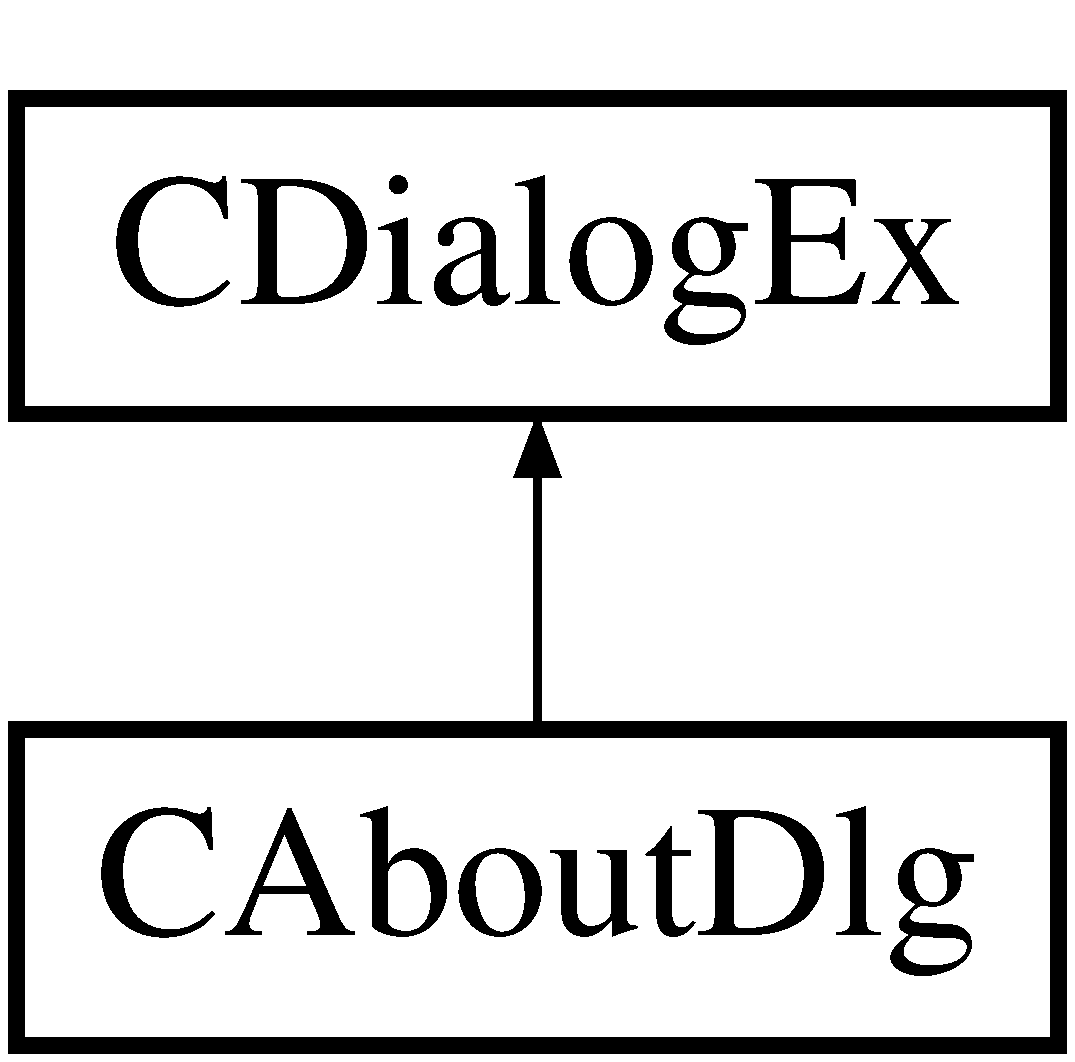
\includegraphics[height=2.000000cm]{class_c_about_dlg}
\end{center}
\end{figure}
\subsection*{Public Types}
\begin{DoxyCompactItemize}
\item 
\hypertarget{class_c_about_dlg_a27a5d4c47f16acb8562522fcd22871f7}{enum \{ {\bfseries I\+D\+D} = I\+D\+D\+\_\+\+A\+B\+O\+U\+T\+B\+O\+X
 \}}\label{class_c_about_dlg_a27a5d4c47f16acb8562522fcd22871f7}

\end{DoxyCompactItemize}
\subsection*{Public Member Functions}
\begin{DoxyCompactItemize}
\item 
\hypertarget{class_c_about_dlg_a6d1e6a33fef23bee6e75254189d865ce}{\hyperlink{class_c_about_dlg_a6d1e6a33fef23bee6e75254189d865ce}{C\+About\+Dlg} ()}\label{class_c_about_dlg_a6d1e6a33fef23bee6e75254189d865ce}

\begin{DoxyCompactList}\small\item\em Constructor. \end{DoxyCompactList}\end{DoxyCompactItemize}
\subsection*{Protected Member Functions}
\begin{DoxyCompactItemize}
\item 
virtual void \hyperlink{class_c_about_dlg_ab83db7484fec957282d7d5a21aed4df4}{Do\+Data\+Exchange} (C\+Data\+Exchange $\ast$p\+D\+X)
\begin{DoxyCompactList}\small\item\em Exchange data between the class and the dialog box. \end{DoxyCompactList}\end{DoxyCompactItemize}


\subsection{Detailed Description}
The About dialog box. 

\subsection{Member Function Documentation}
\hypertarget{class_c_about_dlg_ab83db7484fec957282d7d5a21aed4df4}{\index{C\+About\+Dlg@{C\+About\+Dlg}!Do\+Data\+Exchange@{Do\+Data\+Exchange}}
\index{Do\+Data\+Exchange@{Do\+Data\+Exchange}!C\+About\+Dlg@{C\+About\+Dlg}}
\subsubsection[{Do\+Data\+Exchange}]{\setlength{\rightskip}{0pt plus 5cm}void C\+About\+Dlg\+::\+Do\+Data\+Exchange (
\begin{DoxyParamCaption}
\item[{C\+Data\+Exchange $\ast$}]{p\+D\+X}
\end{DoxyParamCaption}
)\hspace{0.3cm}{\ttfamily [protected]}, {\ttfamily [virtual]}}}\label{class_c_about_dlg_ab83db7484fec957282d7d5a21aed4df4}


Exchange data between the class and the dialog box. 


\begin{DoxyParams}{Parameters}
{\em p\+D\+X} & structure that controls the data exchange \\
\hline
\end{DoxyParams}


The documentation for this class was generated from the following file\+:\begin{DoxyCompactItemize}
\item 
\hyperlink{_canadian_experience_8cpp}{Canadian\+Experience.\+cpp}\end{DoxyCompactItemize}

\hypertarget{class_c_actor}{\section{C\+Actor Class Reference}
\label{class_c_actor}\index{C\+Actor@{C\+Actor}}
}


Class for actors in our drawings.  




{\ttfamily \#include $<$Actor.\+h$>$}

\subsection*{Public Member Functions}
\begin{DoxyCompactItemize}
\item 
\hyperlink{class_c_actor_a26b1abd4ebd92942ae67af59abd9e4d2}{C\+Actor} (const wstring \&name)
\begin{DoxyCompactList}\small\item\em Non-\/default constructor. \end{DoxyCompactList}\item 
\hyperlink{class_c_actor_ae7683d5f0b3edc85dc47850fa71de40f}{C\+Actor} ()=delete
\begin{DoxyCompactList}\small\item\em Disable default constructor. \end{DoxyCompactList}\item 
\hypertarget{class_c_actor_a8af986ad4ec530967f942aaebd853632}{\hyperlink{class_c_actor_a8af986ad4ec530967f942aaebd853632}{C\+Actor} (const \hyperlink{class_c_actor}{C\+Actor} \&)=delete}\label{class_c_actor_a8af986ad4ec530967f942aaebd853632}

\begin{DoxyCompactList}\small\item\em Delete the copy constructor. \end{DoxyCompactList}\item 
\hypertarget{class_c_actor_ab872dc4722654170e427a18da1435e8b}{\hyperlink{class_c_actor}{C\+Actor} \& \hyperlink{class_c_actor_ab872dc4722654170e427a18da1435e8b}{operator=} (const \hyperlink{class_c_actor}{C\+Actor} \&)=delete}\label{class_c_actor_ab872dc4722654170e427a18da1435e8b}

\begin{DoxyCompactList}\small\item\em Delete the assignment operator. \end{DoxyCompactList}\item 
\hypertarget{class_c_actor_adca86a138fd9af275352336848ebad27}{virtual \hyperlink{class_c_actor_adca86a138fd9af275352336848ebad27}{$\sim$\+C\+Actor} ()}\label{class_c_actor_adca86a138fd9af275352336848ebad27}

\begin{DoxyCompactList}\small\item\em Virtual Destructor. \end{DoxyCompactList}\item 
void \hyperlink{class_c_actor_add04012d09640195e7dd0f98d80c5bfe}{Draw} (Graphics $\ast$graphics)
\begin{DoxyCompactList}\small\item\em Draws our actor. \end{DoxyCompactList}\item 
shared\+\_\+ptr$<$ \hyperlink{class_c_drawable}{C\+Drawable} $>$ \hyperlink{class_c_actor_a3afe52edb79961f1eb90c82b931ca766}{Hit\+Test} (Point pos)
\begin{DoxyCompactList}\small\item\em A hit test for our actor. \end{DoxyCompactList}\item 
void \hyperlink{class_c_actor_a338b3d46841013baea7f86fdb6f58dc7}{Add\+Drawable} (shared\+\_\+ptr$<$ \hyperlink{class_c_drawable}{C\+Drawable} $>$ drawable)
\begin{DoxyCompactList}\small\item\em Adds a drawable to our actor. \end{DoxyCompactList}\item 
bool \hyperlink{class_c_actor_ab3e78932aeb9e2a764670bc82ac85094}{Is\+Enabled} () const 
\begin{DoxyCompactList}\small\item\em Actor is enabled. \end{DoxyCompactList}\item 
void \hyperlink{class_c_actor_a385a9ac85a6e0f5c0cb2f96109f26ae4}{Set\+Root} (shared\+\_\+ptr$<$ \hyperlink{class_c_drawable}{C\+Drawable} $>$ root)
\begin{DoxyCompactList}\small\item\em Sets the root of our actor. \end{DoxyCompactList}\item 
wstring \hyperlink{class_c_actor_a043ed1819e96171b06a916e5891e953f}{Get\+Name} () const 
\begin{DoxyCompactList}\small\item\em Gets our actors name. \end{DoxyCompactList}\item 
bool \hyperlink{class_c_actor_a54ef050d02a6d25f5bfc8ca9b09f18bf}{Get\+Enabled} () const 
\begin{DoxyCompactList}\small\item\em Gets the enabled flag. \end{DoxyCompactList}\item 
void \hyperlink{class_c_actor_a6f9009e9753b07a00266cac01af2fdad}{Set\+Enabled} (bool enabled)
\begin{DoxyCompactList}\small\item\em Set Actor Enabled. \end{DoxyCompactList}\item 
Point \hyperlink{class_c_actor_a0e87214ef13b3e00e3869b262d6a106c}{Get\+Position} () const 
\begin{DoxyCompactList}\small\item\em Returns the position/point of our actor. \end{DoxyCompactList}\item 
void \hyperlink{class_c_actor_a565fa3f4ffbf8ca360d791623a9491de}{Set\+Position} (Point position)
\begin{DoxyCompactList}\small\item\em Sets the position of our actor to a point. \end{DoxyCompactList}\item 
bool \hyperlink{class_c_actor_a54c9188974b6313d8ffcbac17e343263}{Get\+Clickable} () const 
\begin{DoxyCompactList}\small\item\em Returns if the actor is clickable or not. \end{DoxyCompactList}\item 
void \hyperlink{class_c_actor_a14ba1cc069ad2710b4db5d536b152918}{Set\+Clickable} (bool flag)
\begin{DoxyCompactList}\small\item\em Sets the clickable flag. \end{DoxyCompactList}\item 
\hyperlink{class_c_picture}{C\+Picture} $\ast$ \hyperlink{class_c_actor_adba8556f52253d533e71f5c707f11436}{Get\+Picture} () const 
\begin{DoxyCompactList}\small\item\em Returnf our picture. \end{DoxyCompactList}\item 
void \hyperlink{class_c_actor_ac4b2315b3476d4fdc97ba961fdcaa444}{Set\+Picture} (\hyperlink{class_c_picture}{C\+Picture} $\ast$picture)
\begin{DoxyCompactList}\small\item\em Sets our picture. \end{DoxyCompactList}\end{DoxyCompactItemize}


\subsection{Detailed Description}
Class for actors in our drawings. 

An actor is some graphical object that consists of one or more parts. Actors can be animated. 

\subsection{Constructor \& Destructor Documentation}
\hypertarget{class_c_actor_a26b1abd4ebd92942ae67af59abd9e4d2}{\index{C\+Actor@{C\+Actor}!C\+Actor@{C\+Actor}}
\index{C\+Actor@{C\+Actor}!C\+Actor@{C\+Actor}}
\subsubsection[{C\+Actor}]{\setlength{\rightskip}{0pt plus 5cm}C\+Actor\+::\+C\+Actor (
\begin{DoxyParamCaption}
\item[{const wstring \&}]{name}
\end{DoxyParamCaption}
)}}\label{class_c_actor_a26b1abd4ebd92942ae67af59abd9e4d2}


Non-\/default constructor. 

Constructor
\begin{DoxyParams}{Parameters}
{\em name} & -\/ A string to set the actors name as\\
\hline
{\em name} & -\/ A string to set the actors name as \\
\hline
\end{DoxyParams}
\hypertarget{class_c_actor_ae7683d5f0b3edc85dc47850fa71de40f}{\index{C\+Actor@{C\+Actor}!C\+Actor@{C\+Actor}}
\index{C\+Actor@{C\+Actor}!C\+Actor@{C\+Actor}}
\subsubsection[{C\+Actor}]{\setlength{\rightskip}{0pt plus 5cm}C\+Actor\+::\+C\+Actor (
\begin{DoxyParamCaption}
{}
\end{DoxyParamCaption}
)\hspace{0.3cm}{\ttfamily [delete]}}}\label{class_c_actor_ae7683d5f0b3edc85dc47850fa71de40f}


Disable default constructor. 

Removal of Copy, Assignment, and original Constructor 

\subsection{Member Function Documentation}
\hypertarget{class_c_actor_a338b3d46841013baea7f86fdb6f58dc7}{\index{C\+Actor@{C\+Actor}!Add\+Drawable@{Add\+Drawable}}
\index{Add\+Drawable@{Add\+Drawable}!C\+Actor@{C\+Actor}}
\subsubsection[{Add\+Drawable}]{\setlength{\rightskip}{0pt plus 5cm}void C\+Actor\+::\+Add\+Drawable (
\begin{DoxyParamCaption}
\item[{shared\+\_\+ptr$<$ {\bf C\+Drawable} $>$}]{drawable}
\end{DoxyParamCaption}
)}}\label{class_c_actor_a338b3d46841013baea7f86fdb6f58dc7}


Adds a drawable to our actor. 


\begin{DoxyParams}{Parameters}
{\em drawable} & -\/ The \hyperlink{class_c_drawable}{C\+Drawable} object to add to our actor \\
\hline
\end{DoxyParams}
\hypertarget{class_c_actor_add04012d09640195e7dd0f98d80c5bfe}{\index{C\+Actor@{C\+Actor}!Draw@{Draw}}
\index{Draw@{Draw}!C\+Actor@{C\+Actor}}
\subsubsection[{Draw}]{\setlength{\rightskip}{0pt plus 5cm}void C\+Actor\+::\+Draw (
\begin{DoxyParamCaption}
\item[{Graphics $\ast$}]{graphics}
\end{DoxyParamCaption}
)}}\label{class_c_actor_add04012d09640195e7dd0f98d80c5bfe}


Draws our actor. 

General Functions
\begin{DoxyParams}{Parameters}
{\em graphics} & -\/ A graphics context (pointer) to draw upon\\
\hline
{\em graphics} & -\/ A graphics context (pointer) to draw upon \\
\hline
\end{DoxyParams}
\hypertarget{class_c_actor_a54c9188974b6313d8ffcbac17e343263}{\index{C\+Actor@{C\+Actor}!Get\+Clickable@{Get\+Clickable}}
\index{Get\+Clickable@{Get\+Clickable}!C\+Actor@{C\+Actor}}
\subsubsection[{Get\+Clickable}]{\setlength{\rightskip}{0pt plus 5cm}bool C\+Actor\+::\+Get\+Clickable (
\begin{DoxyParamCaption}
{}
\end{DoxyParamCaption}
) const\hspace{0.3cm}{\ttfamily [inline]}}}\label{class_c_actor_a54c9188974b6313d8ffcbac17e343263}


Returns if the actor is clickable or not. 

\begin{DoxyReturn}{Returns}
boolean -\/ Whether we can click the actor or not 
\end{DoxyReturn}
\hypertarget{class_c_actor_a54ef050d02a6d25f5bfc8ca9b09f18bf}{\index{C\+Actor@{C\+Actor}!Get\+Enabled@{Get\+Enabled}}
\index{Get\+Enabled@{Get\+Enabled}!C\+Actor@{C\+Actor}}
\subsubsection[{Get\+Enabled}]{\setlength{\rightskip}{0pt plus 5cm}bool C\+Actor\+::\+Get\+Enabled (
\begin{DoxyParamCaption}
{}
\end{DoxyParamCaption}
) const\hspace{0.3cm}{\ttfamily [inline]}}}\label{class_c_actor_a54ef050d02a6d25f5bfc8ca9b09f18bf}


Gets the enabled flag. 

\begin{DoxyReturn}{Returns}
If the actor is enabled 
\end{DoxyReturn}
\hypertarget{class_c_actor_a043ed1819e96171b06a916e5891e953f}{\index{C\+Actor@{C\+Actor}!Get\+Name@{Get\+Name}}
\index{Get\+Name@{Get\+Name}!C\+Actor@{C\+Actor}}
\subsubsection[{Get\+Name}]{\setlength{\rightskip}{0pt plus 5cm}wstring C\+Actor\+::\+Get\+Name (
\begin{DoxyParamCaption}
{}
\end{DoxyParamCaption}
) const\hspace{0.3cm}{\ttfamily [inline]}}}\label{class_c_actor_a043ed1819e96171b06a916e5891e953f}


Gets our actors name. 

Getters \& Setters\begin{DoxyReturn}{Returns}
String -\/ our actors name 
\end{DoxyReturn}
\hypertarget{class_c_actor_adba8556f52253d533e71f5c707f11436}{\index{C\+Actor@{C\+Actor}!Get\+Picture@{Get\+Picture}}
\index{Get\+Picture@{Get\+Picture}!C\+Actor@{C\+Actor}}
\subsubsection[{Get\+Picture}]{\setlength{\rightskip}{0pt plus 5cm}{\bf C\+Picture}$\ast$ C\+Actor\+::\+Get\+Picture (
\begin{DoxyParamCaption}
{}
\end{DoxyParamCaption}
) const\hspace{0.3cm}{\ttfamily [inline]}}}\label{class_c_actor_adba8556f52253d533e71f5c707f11436}


Returnf our picture. 

\begin{DoxyReturn}{Returns}
\hyperlink{class_c_picture}{C\+Picture} pointer to our picture 
\end{DoxyReturn}
\hypertarget{class_c_actor_a0e87214ef13b3e00e3869b262d6a106c}{\index{C\+Actor@{C\+Actor}!Get\+Position@{Get\+Position}}
\index{Get\+Position@{Get\+Position}!C\+Actor@{C\+Actor}}
\subsubsection[{Get\+Position}]{\setlength{\rightskip}{0pt plus 5cm}Point C\+Actor\+::\+Get\+Position (
\begin{DoxyParamCaption}
{}
\end{DoxyParamCaption}
) const\hspace{0.3cm}{\ttfamily [inline]}}}\label{class_c_actor_a0e87214ef13b3e00e3869b262d6a106c}


Returns the position/point of our actor. 

\begin{DoxyReturn}{Returns}
A point where our actor is located 
\end{DoxyReturn}
\hypertarget{class_c_actor_a3afe52edb79961f1eb90c82b931ca766}{\index{C\+Actor@{C\+Actor}!Hit\+Test@{Hit\+Test}}
\index{Hit\+Test@{Hit\+Test}!C\+Actor@{C\+Actor}}
\subsubsection[{Hit\+Test}]{\setlength{\rightskip}{0pt plus 5cm}shared\+\_\+ptr$<$ {\bf C\+Drawable} $>$ C\+Actor\+::\+Hit\+Test (
\begin{DoxyParamCaption}
\item[{Point}]{pos}
\end{DoxyParamCaption}
)}}\label{class_c_actor_a3afe52edb79961f1eb90c82b931ca766}


A hit test for our actor. 


\begin{DoxyParams}{Parameters}
{\em pos} & -\/ A point to test \\
\hline
\end{DoxyParams}
\begin{DoxyReturn}{Returns}
The object (\hyperlink{class_c_drawable}{C\+Drawable}) that is hit 
\end{DoxyReturn}
\hypertarget{class_c_actor_ab3e78932aeb9e2a764670bc82ac85094}{\index{C\+Actor@{C\+Actor}!Is\+Enabled@{Is\+Enabled}}
\index{Is\+Enabled@{Is\+Enabled}!C\+Actor@{C\+Actor}}
\subsubsection[{Is\+Enabled}]{\setlength{\rightskip}{0pt plus 5cm}bool C\+Actor\+::\+Is\+Enabled (
\begin{DoxyParamCaption}
{}
\end{DoxyParamCaption}
) const\hspace{0.3cm}{\ttfamily [inline]}}}\label{class_c_actor_ab3e78932aeb9e2a764670bc82ac85094}


Actor is enabled. 

\begin{DoxyReturn}{Returns}
enabled status 
\end{DoxyReturn}
\hypertarget{class_c_actor_a14ba1cc069ad2710b4db5d536b152918}{\index{C\+Actor@{C\+Actor}!Set\+Clickable@{Set\+Clickable}}
\index{Set\+Clickable@{Set\+Clickable}!C\+Actor@{C\+Actor}}
\subsubsection[{Set\+Clickable}]{\setlength{\rightskip}{0pt plus 5cm}void C\+Actor\+::\+Set\+Clickable (
\begin{DoxyParamCaption}
\item[{bool}]{flag}
\end{DoxyParamCaption}
)\hspace{0.3cm}{\ttfamily [inline]}}}\label{class_c_actor_a14ba1cc069ad2710b4db5d536b152918}


Sets the clickable flag. 


\begin{DoxyParams}{Parameters}
{\em flag} & -\/ The boolean to set if we can click our actor \\
\hline
\end{DoxyParams}
\hypertarget{class_c_actor_a6f9009e9753b07a00266cac01af2fdad}{\index{C\+Actor@{C\+Actor}!Set\+Enabled@{Set\+Enabled}}
\index{Set\+Enabled@{Set\+Enabled}!C\+Actor@{C\+Actor}}
\subsubsection[{Set\+Enabled}]{\setlength{\rightskip}{0pt plus 5cm}void C\+Actor\+::\+Set\+Enabled (
\begin{DoxyParamCaption}
\item[{bool}]{enabled}
\end{DoxyParamCaption}
)\hspace{0.3cm}{\ttfamily [inline]}}}\label{class_c_actor_a6f9009e9753b07a00266cac01af2fdad}


Set Actor Enabled. 


\begin{DoxyParams}{Parameters}
{\em enabled} & New enabled status \\
\hline
\end{DoxyParams}
\hypertarget{class_c_actor_ac4b2315b3476d4fdc97ba961fdcaa444}{\index{C\+Actor@{C\+Actor}!Set\+Picture@{Set\+Picture}}
\index{Set\+Picture@{Set\+Picture}!C\+Actor@{C\+Actor}}
\subsubsection[{Set\+Picture}]{\setlength{\rightskip}{0pt plus 5cm}void C\+Actor\+::\+Set\+Picture (
\begin{DoxyParamCaption}
\item[{{\bf C\+Picture} $\ast$}]{picture}
\end{DoxyParamCaption}
)\hspace{0.3cm}{\ttfamily [inline]}}}\label{class_c_actor_ac4b2315b3476d4fdc97ba961fdcaa444}


Sets our picture. 


\begin{DoxyParams}{Parameters}
{\em picture} & -\/ The picture to set \\
\hline
\end{DoxyParams}
\hypertarget{class_c_actor_a565fa3f4ffbf8ca360d791623a9491de}{\index{C\+Actor@{C\+Actor}!Set\+Position@{Set\+Position}}
\index{Set\+Position@{Set\+Position}!C\+Actor@{C\+Actor}}
\subsubsection[{Set\+Position}]{\setlength{\rightskip}{0pt plus 5cm}void C\+Actor\+::\+Set\+Position (
\begin{DoxyParamCaption}
\item[{Point}]{position}
\end{DoxyParamCaption}
)\hspace{0.3cm}{\ttfamily [inline]}}}\label{class_c_actor_a565fa3f4ffbf8ca360d791623a9491de}


Sets the position of our actor to a point. 


\begin{DoxyParams}{Parameters}
{\em position} & -\/ The point to set our actor to \\
\hline
\end{DoxyParams}
\hypertarget{class_c_actor_a385a9ac85a6e0f5c0cb2f96109f26ae4}{\index{C\+Actor@{C\+Actor}!Set\+Root@{Set\+Root}}
\index{Set\+Root@{Set\+Root}!C\+Actor@{C\+Actor}}
\subsubsection[{Set\+Root}]{\setlength{\rightskip}{0pt plus 5cm}void C\+Actor\+::\+Set\+Root (
\begin{DoxyParamCaption}
\item[{shared\+\_\+ptr$<$ {\bf C\+Drawable} $>$}]{root}
\end{DoxyParamCaption}
)}}\label{class_c_actor_a385a9ac85a6e0f5c0cb2f96109f26ae4}


Sets the root of our actor. 

Set the root drawable for the actor.


\begin{DoxyParams}{Parameters}
{\em root} & -\/ A drawable object\\
\hline
{\em root} & Pointer to root drawable \\
\hline
\end{DoxyParams}


The documentation for this class was generated from the following files\+:\begin{DoxyCompactItemize}
\item 
\hyperlink{_actor_8h}{Actor.\+h}\item 
\hyperlink{_actor_8cpp}{Actor.\+cpp}\end{DoxyCompactItemize}

\hypertarget{class_c_actor_factory}{\section{C\+Actor\+Factory Class Reference}
\label{class_c_actor_factory}\index{C\+Actor\+Factory@{C\+Actor\+Factory}}
}


Abstract base class for actor factories.  




{\ttfamily \#include $<$Actor\+Factory.\+h$>$}

Inheritance diagram for C\+Actor\+Factory\+:\begin{figure}[H]
\begin{center}
\leavevmode
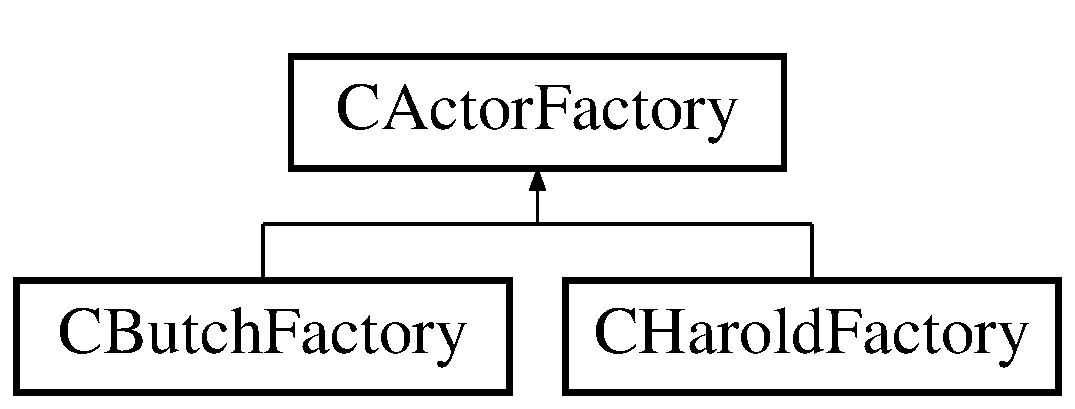
\includegraphics[height=2.000000cm]{class_c_actor_factory}
\end{center}
\end{figure}
\subsection*{Public Member Functions}
\begin{DoxyCompactItemize}
\item 
\hypertarget{class_c_actor_factory_a6a9d84ffa74ef0b01bf1e31fb28efcaa}{\hyperlink{class_c_actor_factory_a6a9d84ffa74ef0b01bf1e31fb28efcaa}{C\+Actor\+Factory} ()}\label{class_c_actor_factory_a6a9d84ffa74ef0b01bf1e31fb28efcaa}

\begin{DoxyCompactList}\small\item\em Constructor. \end{DoxyCompactList}\item 
virtual \hyperlink{class_c_actor_factory_a2c3174c6ca0362dbd3dbd2f599a51c46}{$\sim$\+C\+Actor\+Factory} ()
\begin{DoxyCompactList}\small\item\em Destructor. \end{DoxyCompactList}\end{DoxyCompactItemize}


\subsection{Detailed Description}
Abstract base class for actor factories. 

\subsection{Constructor \& Destructor Documentation}
\hypertarget{class_c_actor_factory_a2c3174c6ca0362dbd3dbd2f599a51c46}{\index{C\+Actor\+Factory@{C\+Actor\+Factory}!````~C\+Actor\+Factory@{$\sim$\+C\+Actor\+Factory}}
\index{````~C\+Actor\+Factory@{$\sim$\+C\+Actor\+Factory}!C\+Actor\+Factory@{C\+Actor\+Factory}}
\subsubsection[{$\sim$\+C\+Actor\+Factory}]{\setlength{\rightskip}{0pt plus 5cm}C\+Actor\+Factory\+::$\sim$\+C\+Actor\+Factory (
\begin{DoxyParamCaption}
{}
\end{DoxyParamCaption}
)\hspace{0.3cm}{\ttfamily [virtual]}}}\label{class_c_actor_factory_a2c3174c6ca0362dbd3dbd2f599a51c46}


Destructor. 

Destructor 

The documentation for this class was generated from the following files\+:\begin{DoxyCompactItemize}
\item 
\hyperlink{_actor_factory_8h}{Actor\+Factory.\+h}\item 
\hyperlink{_actor_factory_8cpp}{Actor\+Factory.\+cpp}\end{DoxyCompactItemize}

\hypertarget{class_c_butch_factory}{\section{C\+Butch\+Factory Class Reference}
\label{class_c_butch_factory}\index{C\+Butch\+Factory@{C\+Butch\+Factory}}
}


Creates a new actor -\/ Butch.  




{\ttfamily \#include $<$Butch\+Factory.\+h$>$}

Inheritance diagram for C\+Butch\+Factory\+:\begin{figure}[H]
\begin{center}
\leavevmode
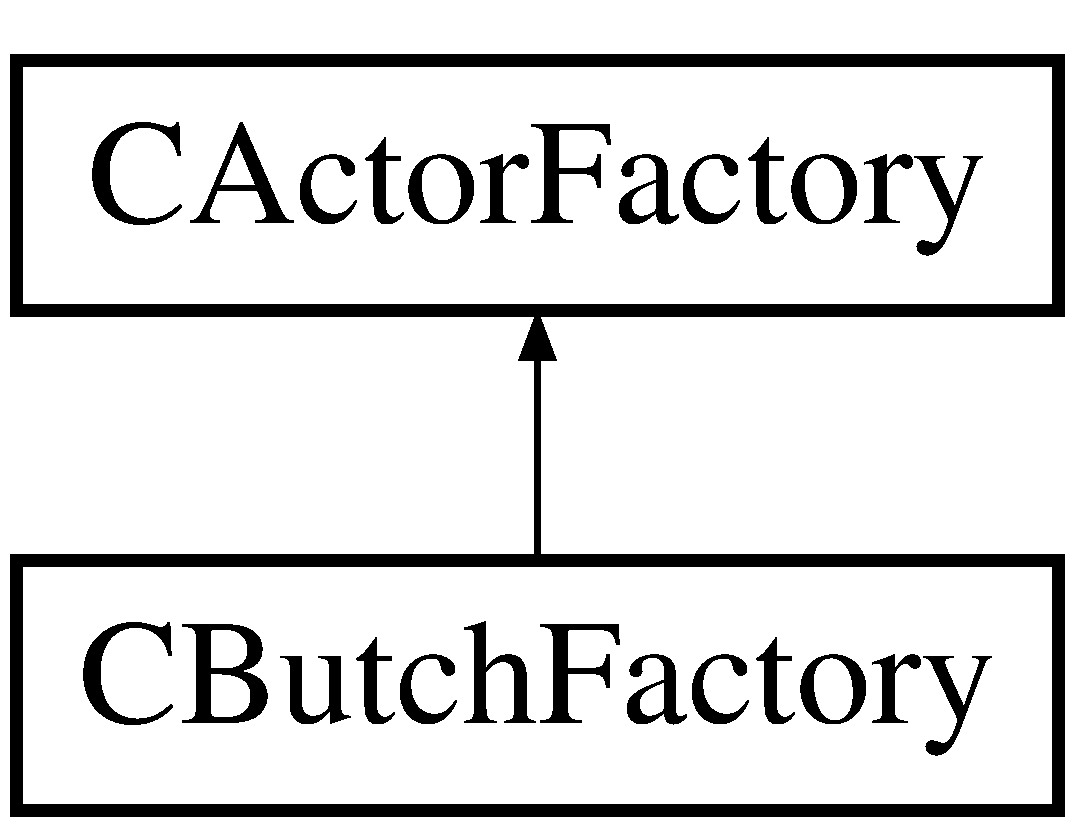
\includegraphics[height=2.000000cm]{class_c_butch_factory}
\end{center}
\end{figure}
\subsection*{Public Member Functions}
\begin{DoxyCompactItemize}
\item 
\hypertarget{class_c_butch_factory_a74990475edd5f1170ad0653123affdde}{\hyperlink{class_c_butch_factory_a74990475edd5f1170ad0653123affdde}{C\+Butch\+Factory} ()}\label{class_c_butch_factory_a74990475edd5f1170ad0653123affdde}

\begin{DoxyCompactList}\small\item\em Constructor. \end{DoxyCompactList}\item 
\hypertarget{class_c_butch_factory_a6d4786123569b4dd03834e9fe2c83d37}{virtual \hyperlink{class_c_butch_factory_a6d4786123569b4dd03834e9fe2c83d37}{$\sim$\+C\+Butch\+Factory} ()}\label{class_c_butch_factory_a6d4786123569b4dd03834e9fe2c83d37}

\begin{DoxyCompactList}\small\item\em Destructor. \end{DoxyCompactList}\item 
std\+::shared\+\_\+ptr$<$ \hyperlink{class_c_actor}{C\+Actor} $>$ \hyperlink{class_c_butch_factory_afe7d27e222c1b49e05dcda4902b3188f}{Create} ()
\begin{DoxyCompactList}\small\item\em Creates a butch. \end{DoxyCompactList}\end{DoxyCompactItemize}


\subsection{Detailed Description}
Creates a new actor -\/ Butch. 

\subsection{Member Function Documentation}
\hypertarget{class_c_butch_factory_afe7d27e222c1b49e05dcda4902b3188f}{\index{C\+Butch\+Factory@{C\+Butch\+Factory}!Create@{Create}}
\index{Create@{Create}!C\+Butch\+Factory@{C\+Butch\+Factory}}
\subsubsection[{Create}]{\setlength{\rightskip}{0pt plus 5cm}std\+::shared\+\_\+ptr$<$ {\bf C\+Actor} $>$ C\+Butch\+Factory\+::\+Create (
\begin{DoxyParamCaption}
{}
\end{DoxyParamCaption}
)}}\label{class_c_butch_factory_afe7d27e222c1b49e05dcda4902b3188f}


Creates a butch. 

This is a concrete factory method that creates our Butch actor.

\begin{DoxyReturn}{Returns}
A shared-\/pointer to our new butch object

Pointer to an actor object. 
\end{DoxyReturn}
Initializing

Creating Parts

Adding Parts 

The documentation for this class was generated from the following files\+:\begin{DoxyCompactItemize}
\item 
\hyperlink{_butch_factory_8h}{Butch\+Factory.\+h}\item 
\hyperlink{_butch_factory_8cpp}{Butch\+Factory.\+cpp}\end{DoxyCompactItemize}

\hypertarget{class_c_canadian_experience_app}{\section{C\+Canadian\+Experience\+App Class Reference}
\label{class_c_canadian_experience_app}\index{C\+Canadian\+Experience\+App@{C\+Canadian\+Experience\+App}}
}


Program application class.  




{\ttfamily \#include $<$Canadian\+Experience.\+h$>$}

Inheritance diagram for C\+Canadian\+Experience\+App\+:\begin{figure}[H]
\begin{center}
\leavevmode
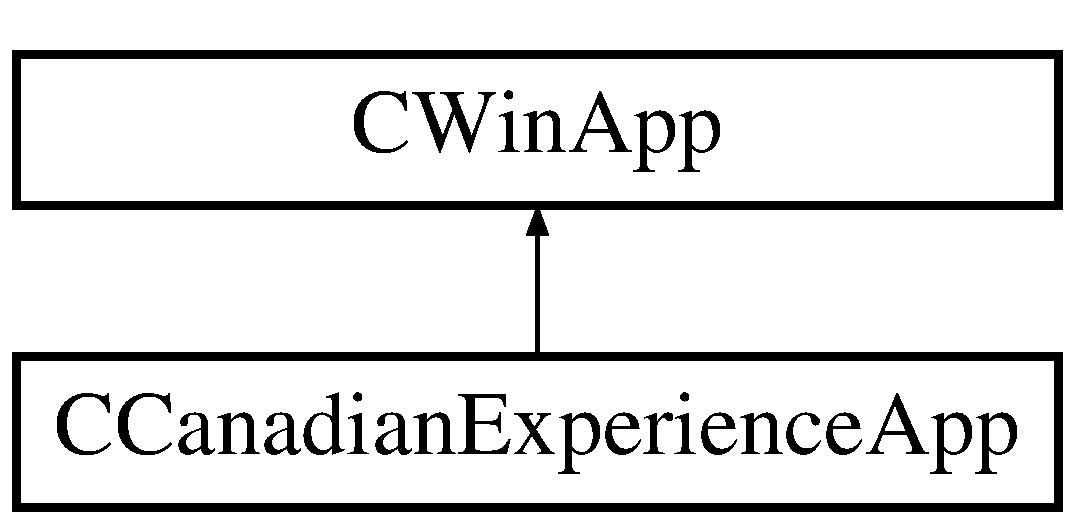
\includegraphics[height=2.000000cm]{class_c_canadian_experience_app}
\end{center}
\end{figure}
\subsection*{Public Member Functions}
\begin{DoxyCompactItemize}
\item 
virtual B\+O\+O\+L \hyperlink{class_c_canadian_experience_app_ab821deed5758f650a2fbbc65cefc8cc7}{Init\+Instance} ()
\begin{DoxyCompactList}\small\item\em \hyperlink{class_c_canadian_experience_app}{C\+Canadian\+Experience\+App} initialization. \end{DoxyCompactList}\item 
virtual int \hyperlink{class_c_canadian_experience_app_a289a9574888e0c922c455e73edf424ad}{Exit\+Instance} ()
\begin{DoxyCompactList}\small\item\em Exit this program. \end{DoxyCompactList}\item 
\hypertarget{class_c_canadian_experience_app_a99cb24a35f65d5821f7e09eefb0c97e7}{afx\+\_\+msg void \hyperlink{class_c_canadian_experience_app_a99cb24a35f65d5821f7e09eefb0c97e7}{On\+App\+About} ()}\label{class_c_canadian_experience_app_a99cb24a35f65d5821f7e09eefb0c97e7}

\begin{DoxyCompactList}\small\item\em App command to run the dialog. \end{DoxyCompactList}\end{DoxyCompactItemize}


\subsection{Detailed Description}
Program application class. 

\subsection{Member Function Documentation}
\hypertarget{class_c_canadian_experience_app_a289a9574888e0c922c455e73edf424ad}{\index{C\+Canadian\+Experience\+App@{C\+Canadian\+Experience\+App}!Exit\+Instance@{Exit\+Instance}}
\index{Exit\+Instance@{Exit\+Instance}!C\+Canadian\+Experience\+App@{C\+Canadian\+Experience\+App}}
\subsubsection[{Exit\+Instance}]{\setlength{\rightskip}{0pt plus 5cm}int C\+Canadian\+Experience\+App\+::\+Exit\+Instance (
\begin{DoxyParamCaption}
{}
\end{DoxyParamCaption}
)\hspace{0.3cm}{\ttfamily [virtual]}}}\label{class_c_canadian_experience_app_a289a9574888e0c922c455e73edf424ad}


Exit this program. 

\begin{DoxyReturn}{Returns}
exit code 
\end{DoxyReturn}
\hypertarget{class_c_canadian_experience_app_ab821deed5758f650a2fbbc65cefc8cc7}{\index{C\+Canadian\+Experience\+App@{C\+Canadian\+Experience\+App}!Init\+Instance@{Init\+Instance}}
\index{Init\+Instance@{Init\+Instance}!C\+Canadian\+Experience\+App@{C\+Canadian\+Experience\+App}}
\subsubsection[{Init\+Instance}]{\setlength{\rightskip}{0pt plus 5cm}B\+O\+O\+L C\+Canadian\+Experience\+App\+::\+Init\+Instance (
\begin{DoxyParamCaption}
{}
\end{DoxyParamCaption}
)\hspace{0.3cm}{\ttfamily [virtual]}}}\label{class_c_canadian_experience_app_ab821deed5758f650a2fbbc65cefc8cc7}


\hyperlink{class_c_canadian_experience_app}{C\+Canadian\+Experience\+App} initialization. 

\begin{DoxyReturn}{Returns}
T\+R\+U\+E if successful 
\end{DoxyReturn}


The documentation for this class was generated from the following files\+:\begin{DoxyCompactItemize}
\item 
\hyperlink{_canadian_experience_8h}{Canadian\+Experience.\+h}\item 
\hyperlink{_canadian_experience_8cpp}{Canadian\+Experience.\+cpp}\end{DoxyCompactItemize}

\hypertarget{class_c_drawable}{\section{C\+Drawable Class Reference}
\label{class_c_drawable}\index{C\+Drawable@{C\+Drawable}}
}


Abstract base class for drawable elements of our picture.  




{\ttfamily \#include $<$Drawable.\+h$>$}

Inheritance diagram for C\+Drawable\+:\begin{figure}[H]
\begin{center}
\leavevmode
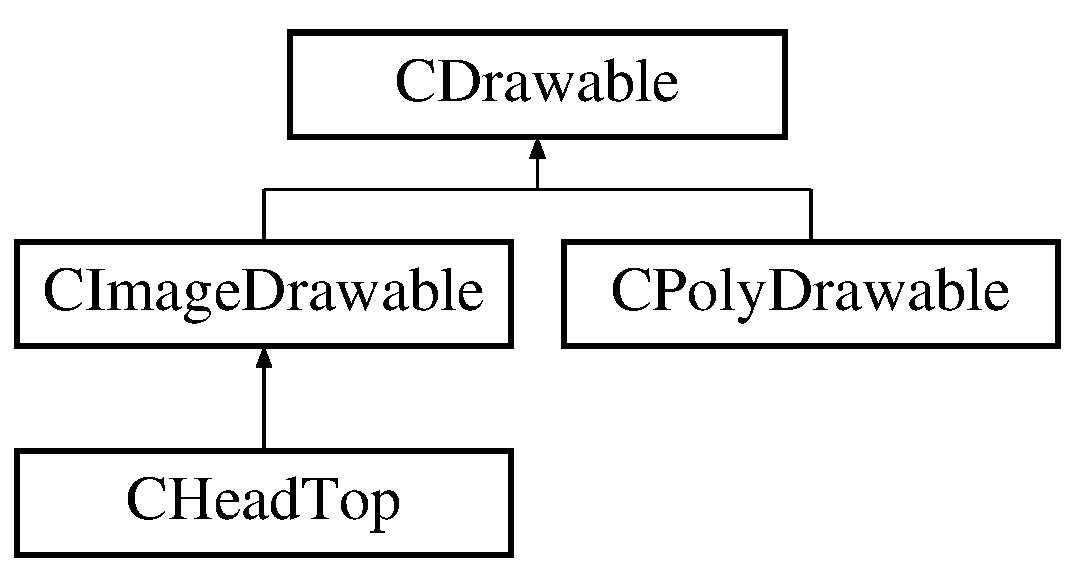
\includegraphics[height=3.000000cm]{class_c_drawable}
\end{center}
\end{figure}
\subsection*{Public Member Functions}
\begin{DoxyCompactItemize}
\item 
\hyperlink{class_c_drawable_abd46d61baf3d5f5210aa3c66b98d9263}{C\+Drawable} ()=delete
\begin{DoxyCompactList}\small\item\em Default constructor disabled. \end{DoxyCompactList}\item 
\hypertarget{class_c_drawable_abec99c088c1a7c12e1d7ecae69135602}{\hyperlink{class_c_drawable_abec99c088c1a7c12e1d7ecae69135602}{C\+Drawable} (const \hyperlink{class_c_drawable}{C\+Drawable} \&)=delete}\label{class_c_drawable_abec99c088c1a7c12e1d7ecae69135602}

\begin{DoxyCompactList}\small\item\em Copy constructor disabled. \end{DoxyCompactList}\item 
\hypertarget{class_c_drawable_aabd5f52b903e57a4c8b145cb69158adb}{void \hyperlink{class_c_drawable_aabd5f52b903e57a4c8b145cb69158adb}{operator=} (const \hyperlink{class_c_drawable}{C\+Drawable} \&)=delete}\label{class_c_drawable_aabd5f52b903e57a4c8b145cb69158adb}

\begin{DoxyCompactList}\small\item\em Assignment operator disabled. \end{DoxyCompactList}\item 
virtual \hyperlink{class_c_drawable_a58fd1036856d627b19976088e4143630}{$\sim$\+C\+Drawable} ()
\begin{DoxyCompactList}\small\item\em Virtual Destructor. \end{DoxyCompactList}\item 
virtual void \hyperlink{class_c_drawable_a9b6a9920a75d88d9ae321997495eaec7}{Draw} (Gdiplus\+::\+Graphics $\ast$graphics)=0
\begin{DoxyCompactList}\small\item\em Draws the drawable. \end{DoxyCompactList}\item 
void \hyperlink{class_c_drawable_ac154be14313b739471d3a1529a2b31b5}{Place} (Gdiplus\+::\+Point offset, double rotate)
\begin{DoxyCompactList}\small\item\em Moves a point. \end{DoxyCompactList}\item 
void \hyperlink{class_c_drawable_ab636167462699dde9b80e6dcb08caf7c}{Add\+Child} (std\+::shared\+\_\+ptr$<$ \hyperlink{class_c_drawable}{C\+Drawable} $>$ child)
\begin{DoxyCompactList}\small\item\em Adds a child. \end{DoxyCompactList}\item 
virtual bool \hyperlink{class_c_drawable_af715bc2e79788b2a44a74ad70b181544}{Hit\+Test} (Gdiplus\+::\+Point pos)=0
\begin{DoxyCompactList}\small\item\em The hit-\/test function for our drawable (pure virtual) \end{DoxyCompactList}\item 
virtual bool \hyperlink{class_c_drawable_ac9f03cfc58aed75fb52cd69c71e7b6e0}{Is\+Movable} ()
\begin{DoxyCompactList}\small\item\em Returns if our drawable is movable. \end{DoxyCompactList}\item 
void \hyperlink{class_c_drawable_a2241b02a5f50c7a455283a9fb24d5b27}{Move} (Gdiplus\+::\+Point delta)
\begin{DoxyCompactList}\small\item\em Moves our drawable based off of a point. \end{DoxyCompactList}\item 
void \hyperlink{class_c_drawable_a86762c6e220d9f502c6ccf9baf1135ac}{Set\+Actor} (\hyperlink{class_c_actor}{C\+Actor} $\ast$actor)
\begin{DoxyCompactList}\small\item\em Sets the actor for this drawable. \end{DoxyCompactList}\item 
void \hyperlink{class_c_drawable_aa6b8988df847a76c30dfcf525ab65449}{Set\+Position} (Gdiplus\+::\+Point pos)
\begin{DoxyCompactList}\small\item\em Set the drawable position. \end{DoxyCompactList}\item 
Gdiplus\+::\+Point \hyperlink{class_c_drawable_ac1def1d34d8069e3985e3a423ba80f2d}{Get\+Position} () const 
\begin{DoxyCompactList}\small\item\em Get the drawable position. \end{DoxyCompactList}\item 
void \hyperlink{class_c_drawable_ab1191ba99b869690839ff20cd0cc45c4}{Set\+Rotation} (double r)
\begin{DoxyCompactList}\small\item\em Set the rotation angle in radians. \end{DoxyCompactList}\item 
double \hyperlink{class_c_drawable_afb31912cfe47cc336dfbef384181ca65}{Get\+Rotation} () const 
\begin{DoxyCompactList}\small\item\em Get the rotation angle in radians. \end{DoxyCompactList}\item 
std\+::wstring \hyperlink{class_c_drawable_a45af045c285cd0be9340a9a0d9883260}{Get\+Name} () const 
\begin{DoxyCompactList}\small\item\em Get the drawable name. \end{DoxyCompactList}\item 
void \hyperlink{class_c_drawable_ad53fc2430248f2ac022ab142024df983}{Set\+Parent} (\hyperlink{class_c_drawable}{C\+Drawable} $\ast$parent)
\begin{DoxyCompactList}\small\item\em Sets the parent of a child. \end{DoxyCompactList}\item 
\hyperlink{class_c_drawable}{C\+Drawable} $\ast$ \hyperlink{class_c_drawable_ab09e86c9bb408d5e2756ab6b439a674c}{Get\+Parent} () const 
\begin{DoxyCompactList}\small\item\em Gets the parent of a child (if exists) \end{DoxyCompactList}\end{DoxyCompactItemize}
\subsection*{Protected Member Functions}
\begin{DoxyCompactItemize}
\item 
\hyperlink{class_c_drawable_a2e153d7fd3a752139b0b87ea990a25fc}{C\+Drawable} (const std\+::wstring \&name)
\begin{DoxyCompactList}\small\item\em Our constructor. \end{DoxyCompactList}\item 
Point \hyperlink{class_c_drawable_a3dbe65175c065abcba67ea820b42c927}{Rotate\+Point} (Point point, double angle)
\begin{DoxyCompactList}\small\item\em Function for rotating a point. \end{DoxyCompactList}\end{DoxyCompactItemize}
\subsection*{Protected Attributes}
\begin{DoxyCompactItemize}
\item 
\hypertarget{class_c_drawable_af10549c681fe73d2f86885019a06d913}{Point \hyperlink{class_c_drawable_af10549c681fe73d2f86885019a06d913}{m\+Placed\+Position} = Point(0, 0)}\label{class_c_drawable_af10549c681fe73d2f86885019a06d913}

\begin{DoxyCompactList}\small\item\em The actual position in the drawing. \end{DoxyCompactList}\item 
\hypertarget{class_c_drawable_a3b280b16b1a4a8c6e2588b1dc5574bda}{double \hyperlink{class_c_drawable_a3b280b16b1a4a8c6e2588b1dc5574bda}{m\+Placed\+R} = 0}\label{class_c_drawable_a3b280b16b1a4a8c6e2588b1dc5574bda}

\begin{DoxyCompactList}\small\item\em The actual rotation of our drawable. \end{DoxyCompactList}\end{DoxyCompactItemize}


\subsection{Detailed Description}
Abstract base class for drawable elements of our picture. 

A drawable is one part of an actor. Drawable parts can be moved independently. 

\subsection{Constructor \& Destructor Documentation}
\hypertarget{class_c_drawable_abd46d61baf3d5f5210aa3c66b98d9263}{\index{C\+Drawable@{C\+Drawable}!C\+Drawable@{C\+Drawable}}
\index{C\+Drawable@{C\+Drawable}!C\+Drawable@{C\+Drawable}}
\subsubsection[{C\+Drawable}]{\setlength{\rightskip}{0pt plus 5cm}C\+Drawable\+::\+C\+Drawable (
\begin{DoxyParamCaption}
{}
\end{DoxyParamCaption}
)\hspace{0.3cm}{\ttfamily [delete]}}}\label{class_c_drawable_abd46d61baf3d5f5210aa3c66b98d9263}


Default constructor disabled. 

Removal of Constructor Default, Copy, and Assignment \hypertarget{class_c_drawable_a58fd1036856d627b19976088e4143630}{\index{C\+Drawable@{C\+Drawable}!````~C\+Drawable@{$\sim$\+C\+Drawable}}
\index{````~C\+Drawable@{$\sim$\+C\+Drawable}!C\+Drawable@{C\+Drawable}}
\subsubsection[{$\sim$\+C\+Drawable}]{\setlength{\rightskip}{0pt plus 5cm}C\+Drawable\+::$\sim$\+C\+Drawable (
\begin{DoxyParamCaption}
{}
\end{DoxyParamCaption}
)\hspace{0.3cm}{\ttfamily [virtual]}}}\label{class_c_drawable_a58fd1036856d627b19976088e4143630}


Virtual Destructor. 

Destructor. \hypertarget{class_c_drawable_a2e153d7fd3a752139b0b87ea990a25fc}{\index{C\+Drawable@{C\+Drawable}!C\+Drawable@{C\+Drawable}}
\index{C\+Drawable@{C\+Drawable}!C\+Drawable@{C\+Drawable}}
\subsubsection[{C\+Drawable}]{\setlength{\rightskip}{0pt plus 5cm}C\+Drawable\+::\+C\+Drawable (
\begin{DoxyParamCaption}
\item[{const std\+::wstring \&}]{name}
\end{DoxyParamCaption}
)\hspace{0.3cm}{\ttfamily [protected]}}}\label{class_c_drawable_a2e153d7fd3a752139b0b87ea990a25fc}


Our constructor. 

Constructor.


\begin{DoxyParams}{Parameters}
{\em name} & -\/ Our drawable's name to be set\\
\hline
{\em name} & The drawable name \\
\hline
\end{DoxyParams}


\subsection{Member Function Documentation}
\hypertarget{class_c_drawable_ab636167462699dde9b80e6dcb08caf7c}{\index{C\+Drawable@{C\+Drawable}!Add\+Child@{Add\+Child}}
\index{Add\+Child@{Add\+Child}!C\+Drawable@{C\+Drawable}}
\subsubsection[{Add\+Child}]{\setlength{\rightskip}{0pt plus 5cm}void C\+Drawable\+::\+Add\+Child (
\begin{DoxyParamCaption}
\item[{std\+::shared\+\_\+ptr$<$ {\bf C\+Drawable} $>$}]{child}
\end{DoxyParamCaption}
)}}\label{class_c_drawable_ab636167462699dde9b80e6dcb08caf7c}


Adds a child. 

Add a child drawable to this drawable.


\begin{DoxyParams}{Parameters}
{\em child} & -\/ The child to add\\
\hline
{\em child} & The child to add \\
\hline
\end{DoxyParams}
\hypertarget{class_c_drawable_a9b6a9920a75d88d9ae321997495eaec7}{\index{C\+Drawable@{C\+Drawable}!Draw@{Draw}}
\index{Draw@{Draw}!C\+Drawable@{C\+Drawable}}
\subsubsection[{Draw}]{\setlength{\rightskip}{0pt plus 5cm}virtual void C\+Drawable\+::\+Draw (
\begin{DoxyParamCaption}
\item[{Gdiplus\+::\+Graphics $\ast$}]{graphics}
\end{DoxyParamCaption}
)\hspace{0.3cm}{\ttfamily [pure virtual]}}}\label{class_c_drawable_a9b6a9920a75d88d9ae321997495eaec7}


Draws the drawable. 

General Functions
\begin{DoxyParams}{Parameters}
{\em graphics} & -\/ The graphics context to draw in \\
\hline
\end{DoxyParams}
\hypertarget{class_c_drawable_a45af045c285cd0be9340a9a0d9883260}{\index{C\+Drawable@{C\+Drawable}!Get\+Name@{Get\+Name}}
\index{Get\+Name@{Get\+Name}!C\+Drawable@{C\+Drawable}}
\subsubsection[{Get\+Name}]{\setlength{\rightskip}{0pt plus 5cm}std\+::wstring C\+Drawable\+::\+Get\+Name (
\begin{DoxyParamCaption}
{}
\end{DoxyParamCaption}
) const\hspace{0.3cm}{\ttfamily [inline]}}}\label{class_c_drawable_a45af045c285cd0be9340a9a0d9883260}


Get the drawable name. 

\begin{DoxyReturn}{Returns}
The drawable name 
\end{DoxyReturn}
\hypertarget{class_c_drawable_ab09e86c9bb408d5e2756ab6b439a674c}{\index{C\+Drawable@{C\+Drawable}!Get\+Parent@{Get\+Parent}}
\index{Get\+Parent@{Get\+Parent}!C\+Drawable@{C\+Drawable}}
\subsubsection[{Get\+Parent}]{\setlength{\rightskip}{0pt plus 5cm}{\bf C\+Drawable}$\ast$ C\+Drawable\+::\+Get\+Parent (
\begin{DoxyParamCaption}
{}
\end{DoxyParamCaption}
) const\hspace{0.3cm}{\ttfamily [inline]}}}\label{class_c_drawable_ab09e86c9bb408d5e2756ab6b439a674c}


Gets the parent of a child (if exists) 

\begin{DoxyReturn}{Returns}
Pointer to the parent 
\end{DoxyReturn}
\hypertarget{class_c_drawable_ac1def1d34d8069e3985e3a423ba80f2d}{\index{C\+Drawable@{C\+Drawable}!Get\+Position@{Get\+Position}}
\index{Get\+Position@{Get\+Position}!C\+Drawable@{C\+Drawable}}
\subsubsection[{Get\+Position}]{\setlength{\rightskip}{0pt plus 5cm}Gdiplus\+::\+Point C\+Drawable\+::\+Get\+Position (
\begin{DoxyParamCaption}
{}
\end{DoxyParamCaption}
) const\hspace{0.3cm}{\ttfamily [inline]}}}\label{class_c_drawable_ac1def1d34d8069e3985e3a423ba80f2d}


Get the drawable position. 

\begin{DoxyReturn}{Returns}
The drawable position 
\end{DoxyReturn}
\hypertarget{class_c_drawable_afb31912cfe47cc336dfbef384181ca65}{\index{C\+Drawable@{C\+Drawable}!Get\+Rotation@{Get\+Rotation}}
\index{Get\+Rotation@{Get\+Rotation}!C\+Drawable@{C\+Drawable}}
\subsubsection[{Get\+Rotation}]{\setlength{\rightskip}{0pt plus 5cm}double C\+Drawable\+::\+Get\+Rotation (
\begin{DoxyParamCaption}
{}
\end{DoxyParamCaption}
) const\hspace{0.3cm}{\ttfamily [inline]}}}\label{class_c_drawable_afb31912cfe47cc336dfbef384181ca65}


Get the rotation angle in radians. 

\begin{DoxyReturn}{Returns}
The rotation angle in radians 
\end{DoxyReturn}
\hypertarget{class_c_drawable_af715bc2e79788b2a44a74ad70b181544}{\index{C\+Drawable@{C\+Drawable}!Hit\+Test@{Hit\+Test}}
\index{Hit\+Test@{Hit\+Test}!C\+Drawable@{C\+Drawable}}
\subsubsection[{Hit\+Test}]{\setlength{\rightskip}{0pt plus 5cm}virtual bool C\+Drawable\+::\+Hit\+Test (
\begin{DoxyParamCaption}
\item[{Gdiplus\+::\+Point}]{pos}
\end{DoxyParamCaption}
)\hspace{0.3cm}{\ttfamily [pure virtual]}}}\label{class_c_drawable_af715bc2e79788b2a44a74ad70b181544}


The hit-\/test function for our drawable (pure virtual) 


\begin{DoxyParams}{Parameters}
{\em pos} & -\/ The position to test for hit \\
\hline
\end{DoxyParams}
\begin{DoxyReturn}{Returns}
bool -\/ If we hit something 
\end{DoxyReturn}
\hypertarget{class_c_drawable_ac9f03cfc58aed75fb52cd69c71e7b6e0}{\index{C\+Drawable@{C\+Drawable}!Is\+Movable@{Is\+Movable}}
\index{Is\+Movable@{Is\+Movable}!C\+Drawable@{C\+Drawable}}
\subsubsection[{Is\+Movable}]{\setlength{\rightskip}{0pt plus 5cm}virtual bool C\+Drawable\+::\+Is\+Movable (
\begin{DoxyParamCaption}
{}
\end{DoxyParamCaption}
)\hspace{0.3cm}{\ttfamily [inline]}, {\ttfamily [virtual]}}}\label{class_c_drawable_ac9f03cfc58aed75fb52cd69c71e7b6e0}


Returns if our drawable is movable. 

\begin{DoxyReturn}{Returns}
bool -\/ If the object can be moved 
\end{DoxyReturn}


Reimplemented in \hyperlink{class_c_head_top_a38d98789668f640fa3bbb8352fb54c49}{C\+Head\+Top}.

\hypertarget{class_c_drawable_a2241b02a5f50c7a455283a9fb24d5b27}{\index{C\+Drawable@{C\+Drawable}!Move@{Move}}
\index{Move@{Move}!C\+Drawable@{C\+Drawable}}
\subsubsection[{Move}]{\setlength{\rightskip}{0pt plus 5cm}void C\+Drawable\+::\+Move (
\begin{DoxyParamCaption}
\item[{Gdiplus\+::\+Point}]{delta}
\end{DoxyParamCaption}
)}}\label{class_c_drawable_a2241b02a5f50c7a455283a9fb24d5b27}


Moves our drawable based off of a point. 

Move this drawable some amount.


\begin{DoxyParams}{Parameters}
{\em delta} & -\/ A point\\
\hline
{\em delta} & The amount to move \\
\hline
\end{DoxyParams}
\hypertarget{class_c_drawable_ac154be14313b739471d3a1529a2b31b5}{\index{C\+Drawable@{C\+Drawable}!Place@{Place}}
\index{Place@{Place}!C\+Drawable@{C\+Drawable}}
\subsubsection[{Place}]{\setlength{\rightskip}{0pt plus 5cm}void C\+Drawable\+::\+Place (
\begin{DoxyParamCaption}
\item[{Gdiplus\+::\+Point}]{offset, }
\item[{double}]{rotate}
\end{DoxyParamCaption}
)}}\label{class_c_drawable_ac154be14313b739471d3a1529a2b31b5}


Moves a point. 

Place this drawable relative to its parent.


\begin{DoxyParams}{Parameters}
{\em offset} & -\/ The point to choose \\
\hline
{\em rotate} & -\/ how much to rotate by\\
\hline
\end{DoxyParams}
This works hierarchically from top item down. 
\begin{DoxyParams}{Parameters}
{\em offset} & Parent offset \\
\hline
{\em rotate} & Parent rotation \\
\hline
\end{DoxyParams}
\hypertarget{class_c_drawable_a3dbe65175c065abcba67ea820b42c927}{\index{C\+Drawable@{C\+Drawable}!Rotate\+Point@{Rotate\+Point}}
\index{Rotate\+Point@{Rotate\+Point}!C\+Drawable@{C\+Drawable}}
\subsubsection[{Rotate\+Point}]{\setlength{\rightskip}{0pt plus 5cm}Gdiplus\+::\+Point C\+Drawable\+::\+Rotate\+Point (
\begin{DoxyParamCaption}
\item[{Point}]{point, }
\item[{double}]{angle}
\end{DoxyParamCaption}
)\hspace{0.3cm}{\ttfamily [protected]}}}\label{class_c_drawable_a3dbe65175c065abcba67ea820b42c927}


Function for rotating a point. 

Rotate a point by a given angle.


\begin{DoxyParams}{Parameters}
{\em point} & -\/ the point to rotate \\
\hline
{\em angle} & -\/ the angle to rotate by \\
\hline
\end{DoxyParams}
\begin{DoxyReturn}{Returns}
A rotated point
\end{DoxyReturn}

\begin{DoxyParams}{Parameters}
{\em point} & The point to rotate \\
\hline
{\em angle} & An angle in radians \\
\hline
\end{DoxyParams}
\begin{DoxyReturn}{Returns}
Rotated point 
\end{DoxyReturn}
\hypertarget{class_c_drawable_a86762c6e220d9f502c6ccf9baf1135ac}{\index{C\+Drawable@{C\+Drawable}!Set\+Actor@{Set\+Actor}}
\index{Set\+Actor@{Set\+Actor}!C\+Drawable@{C\+Drawable}}
\subsubsection[{Set\+Actor}]{\setlength{\rightskip}{0pt plus 5cm}void C\+Drawable\+::\+Set\+Actor (
\begin{DoxyParamCaption}
\item[{{\bf C\+Actor} $\ast$}]{actor}
\end{DoxyParamCaption}
)}}\label{class_c_drawable_a86762c6e220d9f502c6ccf9baf1135ac}


Sets the actor for this drawable. 

Set the actor using this drawable.

Getters \& Setters
\begin{DoxyParams}{Parameters}
{\em actor} & -\/ A pointer to the actor we are selecting\\
\hline
{\em actor} & Actor using this drawable \\
\hline
\end{DoxyParams}
\hypertarget{class_c_drawable_ad53fc2430248f2ac022ab142024df983}{\index{C\+Drawable@{C\+Drawable}!Set\+Parent@{Set\+Parent}}
\index{Set\+Parent@{Set\+Parent}!C\+Drawable@{C\+Drawable}}
\subsubsection[{Set\+Parent}]{\setlength{\rightskip}{0pt plus 5cm}void C\+Drawable\+::\+Set\+Parent (
\begin{DoxyParamCaption}
\item[{{\bf C\+Drawable} $\ast$}]{parent}
\end{DoxyParamCaption}
)\hspace{0.3cm}{\ttfamily [inline]}}}\label{class_c_drawable_ad53fc2430248f2ac022ab142024df983}


Sets the parent of a child. 


\begin{DoxyParams}{Parameters}
{\em parent} & -\/ Pointer to the parent \\
\hline
\end{DoxyParams}
\hypertarget{class_c_drawable_aa6b8988df847a76c30dfcf525ab65449}{\index{C\+Drawable@{C\+Drawable}!Set\+Position@{Set\+Position}}
\index{Set\+Position@{Set\+Position}!C\+Drawable@{C\+Drawable}}
\subsubsection[{Set\+Position}]{\setlength{\rightskip}{0pt plus 5cm}void C\+Drawable\+::\+Set\+Position (
\begin{DoxyParamCaption}
\item[{Gdiplus\+::\+Point}]{pos}
\end{DoxyParamCaption}
)\hspace{0.3cm}{\ttfamily [inline]}}}\label{class_c_drawable_aa6b8988df847a76c30dfcf525ab65449}


Set the drawable position. 


\begin{DoxyParams}{Parameters}
{\em pos} & The new drawable position \\
\hline
\end{DoxyParams}
\hypertarget{class_c_drawable_ab1191ba99b869690839ff20cd0cc45c4}{\index{C\+Drawable@{C\+Drawable}!Set\+Rotation@{Set\+Rotation}}
\index{Set\+Rotation@{Set\+Rotation}!C\+Drawable@{C\+Drawable}}
\subsubsection[{Set\+Rotation}]{\setlength{\rightskip}{0pt plus 5cm}void C\+Drawable\+::\+Set\+Rotation (
\begin{DoxyParamCaption}
\item[{double}]{r}
\end{DoxyParamCaption}
)\hspace{0.3cm}{\ttfamily [inline]}}}\label{class_c_drawable_ab1191ba99b869690839ff20cd0cc45c4}


Set the rotation angle in radians. 


\begin{DoxyParams}{Parameters}
{\em r} & The new rotation angle in radians \\
\hline
\end{DoxyParams}


The documentation for this class was generated from the following files\+:\begin{DoxyCompactItemize}
\item 
\hyperlink{_drawable_8h}{Drawable.\+h}\item 
\hyperlink{_drawable_8cpp}{Drawable.\+cpp}\end{DoxyCompactItemize}

\hypertarget{class_c_harold_factory}{\section{C\+Harold\+Factory Class Reference}
\label{class_c_harold_factory}\index{C\+Harold\+Factory@{C\+Harold\+Factory}}
}


Factory class that builds the Harold character.  




{\ttfamily \#include $<$Harold\+Factory.\+h$>$}

Inheritance diagram for C\+Harold\+Factory\+:\begin{figure}[H]
\begin{center}
\leavevmode
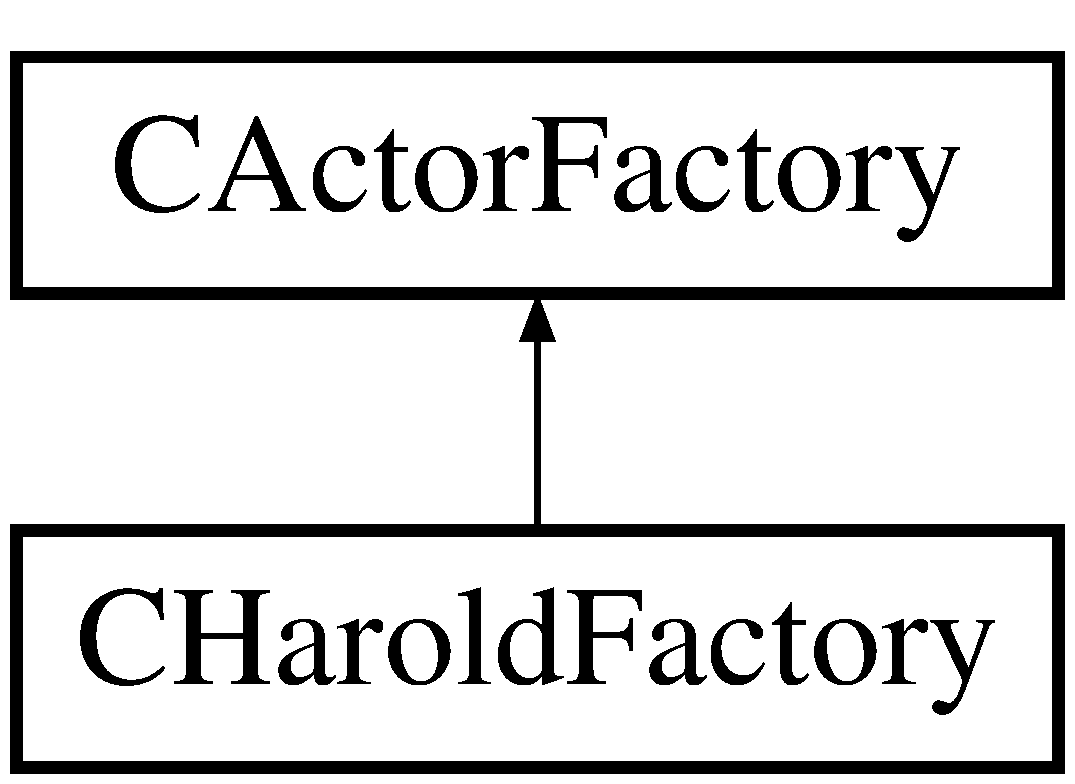
\includegraphics[height=2.000000cm]{class_c_harold_factory}
\end{center}
\end{figure}
\subsection*{Public Member Functions}
\begin{DoxyCompactItemize}
\item 
\hypertarget{class_c_harold_factory_aaa726993be5c432dac2ef22bb06a0bba}{\hyperlink{class_c_harold_factory_aaa726993be5c432dac2ef22bb06a0bba}{C\+Harold\+Factory} ()}\label{class_c_harold_factory_aaa726993be5c432dac2ef22bb06a0bba}

\begin{DoxyCompactList}\small\item\em Constructor. \end{DoxyCompactList}\item 
\hypertarget{class_c_harold_factory_aa2518771a064994af61c159d43788a3b}{virtual \hyperlink{class_c_harold_factory_aa2518771a064994af61c159d43788a3b}{$\sim$\+C\+Harold\+Factory} ()}\label{class_c_harold_factory_aa2518771a064994af61c159d43788a3b}

\begin{DoxyCompactList}\small\item\em Destructor. \end{DoxyCompactList}\item 
std\+::shared\+\_\+ptr$<$ \hyperlink{class_c_actor}{C\+Actor} $>$ \hyperlink{class_c_harold_factory_a785f8194f83d866bfc2a237fc3d4abc1}{Create} ()
\begin{DoxyCompactList}\small\item\em Creates a harold. \end{DoxyCompactList}\end{DoxyCompactItemize}


\subsection{Detailed Description}
Factory class that builds the Harold character. 

\subsection{Member Function Documentation}
\hypertarget{class_c_harold_factory_a785f8194f83d866bfc2a237fc3d4abc1}{\index{C\+Harold\+Factory@{C\+Harold\+Factory}!Create@{Create}}
\index{Create@{Create}!C\+Harold\+Factory@{C\+Harold\+Factory}}
\subsubsection[{Create}]{\setlength{\rightskip}{0pt plus 5cm}std\+::shared\+\_\+ptr$<$ {\bf C\+Actor} $>$ C\+Harold\+Factory\+::\+Create (
\begin{DoxyParamCaption}
{}
\end{DoxyParamCaption}
)}}\label{class_c_harold_factory_a785f8194f83d866bfc2a237fc3d4abc1}


Creates a harold. 

This is a concrete factory method that creates our Harold actor.

\begin{DoxyReturn}{Returns}
A shared-\/pointer to our new harold object

Pointer to an actor object. 
\end{DoxyReturn}


The documentation for this class was generated from the following files\+:\begin{DoxyCompactItemize}
\item 
\hyperlink{_harold_factory_8h}{Harold\+Factory.\+h}\item 
\hyperlink{_harold_factory_8cpp}{Harold\+Factory.\+cpp}\end{DoxyCompactItemize}

\hypertarget{class_c_head_top}{\section{C\+Head\+Top Class Reference}
\label{class_c_head_top}\index{C\+Head\+Top@{C\+Head\+Top}}
}


A class for representing the top of an actor's head.  




{\ttfamily \#include $<$Head\+Top.\+h$>$}

Inheritance diagram for C\+Head\+Top\+:\begin{figure}[H]
\begin{center}
\leavevmode
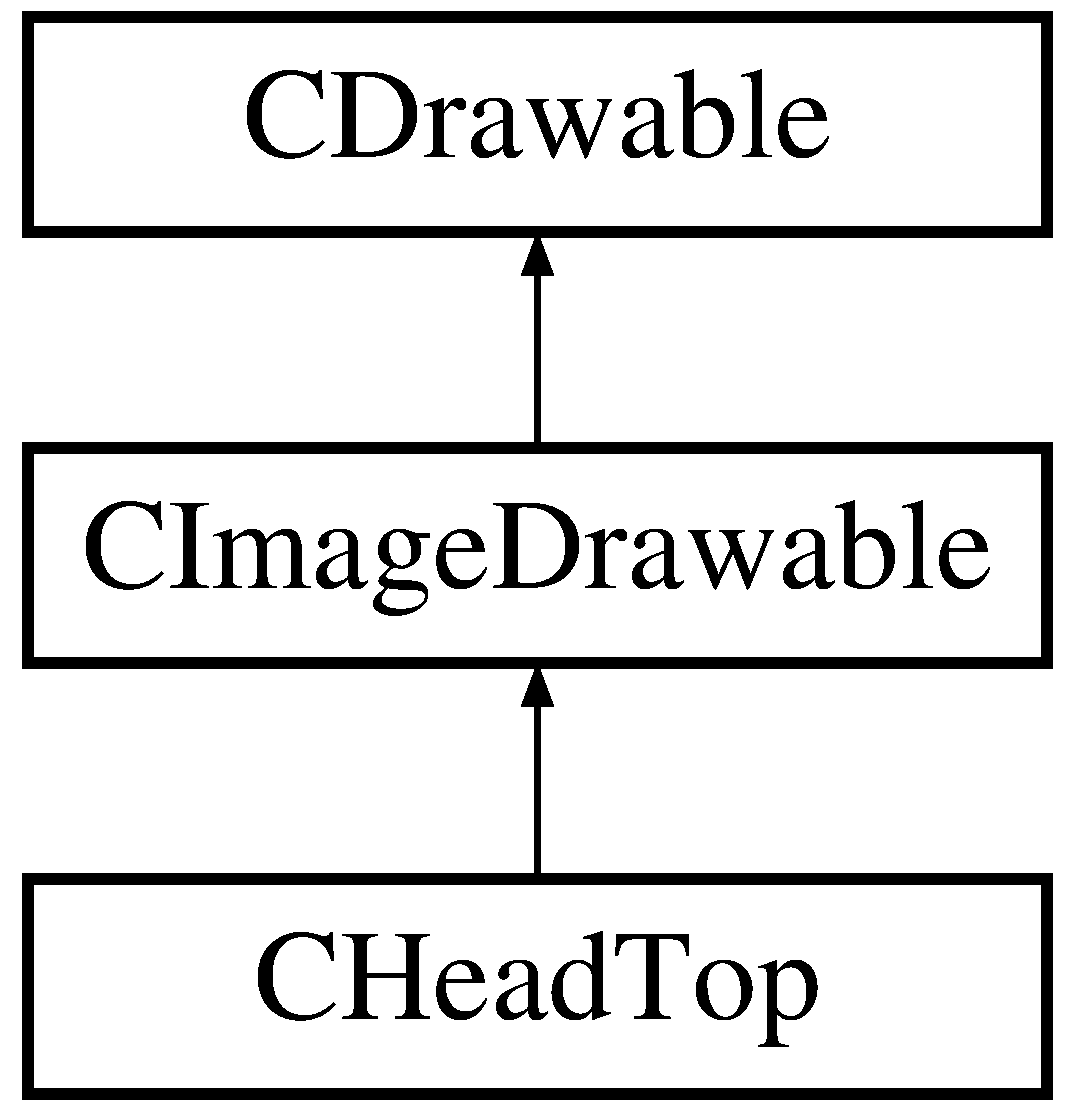
\includegraphics[height=3.000000cm]{class_c_head_top}
\end{center}
\end{figure}
\subsection*{Public Member Functions}
\begin{DoxyCompactItemize}
\item 
\hyperlink{class_c_head_top_a54fab18f42f367ff9cfdf73537ada62f}{C\+Head\+Top} ()=delete
\begin{DoxyCompactList}\small\item\em Default constructor disabled. \end{DoxyCompactList}\item 
\hypertarget{class_c_head_top_a574b5950dff9f90de01219437f475cb9}{\hyperlink{class_c_head_top_a574b5950dff9f90de01219437f475cb9}{C\+Head\+Top} (const \hyperlink{class_c_head_top}{C\+Head\+Top} \&)=delete}\label{class_c_head_top_a574b5950dff9f90de01219437f475cb9}

\begin{DoxyCompactList}\small\item\em Copy constructor disabled. \end{DoxyCompactList}\item 
\hypertarget{class_c_head_top_aeb3522f283f90cb48b7b6a7ed6243aeb}{void \hyperlink{class_c_head_top_aeb3522f283f90cb48b7b6a7ed6243aeb}{operator=} (const \hyperlink{class_c_head_top}{C\+Head\+Top} \&)=delete}\label{class_c_head_top_aeb3522f283f90cb48b7b6a7ed6243aeb}

\begin{DoxyCompactList}\small\item\em Assignment operator disabled. \end{DoxyCompactList}\item 
virtual \hyperlink{class_c_head_top_a64697c81bc0100f66aa661a8bc430fa9}{$\sim$\+C\+Head\+Top} ()
\begin{DoxyCompactList}\small\item\em Destructor. \end{DoxyCompactList}\item 
\hyperlink{class_c_head_top_a31333179dc1836d6ae5b9636b215b66b}{C\+Head\+Top} (const std\+::wstring \&name, const std\+::wstring \&filename)
\begin{DoxyCompactList}\small\item\em Non-\/default Constructor. \end{DoxyCompactList}\item 
void \hyperlink{class_c_head_top_afd29c8fac9d9d44ad4cc2ef480d26d29}{Draw} (Graphics $\ast$graphics)
\begin{DoxyCompactList}\small\item\em Draws our head. \end{DoxyCompactList}\item 
void \hyperlink{class_c_head_top_a8895e3a21b072f335f7e67992eb3bc54}{Draw\+Eyebrow} (Graphics $\ast$graphics, Point location\+Left, Point location\+Right)
\begin{DoxyCompactList}\small\item\em Draws an eyebrow. \end{DoxyCompactList}\item 
void \hyperlink{class_c_head_top_ad00611870a77e747bf6cb03305b027e6}{Draw\+Eye} (Graphics $\ast$graphics, Point location)
\begin{DoxyCompactList}\small\item\em Draws an eye at a location relative to our head top. \end{DoxyCompactList}\item 
bool \hyperlink{class_c_head_top_a38d98789668f640fa3bbb8352fb54c49}{Is\+Movable} () override
\begin{DoxyCompactList}\small\item\em Determines if we can move our head (override) \end{DoxyCompactList}\item 
Point \hyperlink{class_c_head_top_a631542f2cc871fa17542b3253dc6ab73}{Transform\+Point} (Gdiplus\+::\+Point p)
\item 
void \hyperlink{class_c_head_top_aa41cbf785465fde0656348227c44dead}{Set\+Eyes} (Point left\+Eye\+Location, Point right\+Eye\+Location)
\begin{DoxyCompactList}\small\item\em Sets our eye locations. \end{DoxyCompactList}\item 
void \hyperlink{class_c_head_top_a47387e0a6f7317a16bc1492427268f26}{Set\+Left\+Eyebrow} (Point left\+Endpoint, Point right\+Endpoint)
\begin{DoxyCompactList}\small\item\em Sets our left eyebrows left and right endpoints. \end{DoxyCompactList}\item 
void \hyperlink{class_c_head_top_a8743f25295c778d44f899489fee350f1}{Set\+Right\+Eyebrow} (Point left\+Endpoint, Point right\+Endpoint)
\begin{DoxyCompactList}\small\item\em Sets our right eyebrows left and right endpoints. \end{DoxyCompactList}\end{DoxyCompactItemize}
\subsection*{Additional Inherited Members}


\subsection{Detailed Description}
A class for representing the top of an actor's head. 

\subsection{Constructor \& Destructor Documentation}
\hypertarget{class_c_head_top_a54fab18f42f367ff9cfdf73537ada62f}{\index{C\+Head\+Top@{C\+Head\+Top}!C\+Head\+Top@{C\+Head\+Top}}
\index{C\+Head\+Top@{C\+Head\+Top}!C\+Head\+Top@{C\+Head\+Top}}
\subsubsection[{C\+Head\+Top}]{\setlength{\rightskip}{0pt plus 5cm}C\+Head\+Top\+::\+C\+Head\+Top (
\begin{DoxyParamCaption}
{}
\end{DoxyParamCaption}
)\hspace{0.3cm}{\ttfamily [delete]}}}\label{class_c_head_top_a54fab18f42f367ff9cfdf73537ada62f}


Default constructor disabled. 

Delete Default, Copy, Assignemtn \hypertarget{class_c_head_top_a64697c81bc0100f66aa661a8bc430fa9}{\index{C\+Head\+Top@{C\+Head\+Top}!````~C\+Head\+Top@{$\sim$\+C\+Head\+Top}}
\index{````~C\+Head\+Top@{$\sim$\+C\+Head\+Top}!C\+Head\+Top@{C\+Head\+Top}}
\subsubsection[{$\sim$\+C\+Head\+Top}]{\setlength{\rightskip}{0pt plus 5cm}C\+Head\+Top\+::$\sim$\+C\+Head\+Top (
\begin{DoxyParamCaption}
{}
\end{DoxyParamCaption}
)\hspace{0.3cm}{\ttfamily [virtual]}}}\label{class_c_head_top_a64697c81bc0100f66aa661a8bc430fa9}


Destructor. 

Constructor \& Destructor \hypertarget{class_c_head_top_a31333179dc1836d6ae5b9636b215b66b}{\index{C\+Head\+Top@{C\+Head\+Top}!C\+Head\+Top@{C\+Head\+Top}}
\index{C\+Head\+Top@{C\+Head\+Top}!C\+Head\+Top@{C\+Head\+Top}}
\subsubsection[{C\+Head\+Top}]{\setlength{\rightskip}{0pt plus 5cm}C\+Head\+Top\+::\+C\+Head\+Top (
\begin{DoxyParamCaption}
\item[{const std\+::wstring \&}]{name, }
\item[{const std\+::wstring \&}]{filename}
\end{DoxyParamCaption}
)}}\label{class_c_head_top_a31333179dc1836d6ae5b9636b215b66b}


Non-\/default Constructor. 

Constructor. 

\subsection{Member Function Documentation}
\hypertarget{class_c_head_top_afd29c8fac9d9d44ad4cc2ef480d26d29}{\index{C\+Head\+Top@{C\+Head\+Top}!Draw@{Draw}}
\index{Draw@{Draw}!C\+Head\+Top@{C\+Head\+Top}}
\subsubsection[{Draw}]{\setlength{\rightskip}{0pt plus 5cm}void C\+Head\+Top\+::\+Draw (
\begin{DoxyParamCaption}
\item[{Graphics $\ast$}]{graphics}
\end{DoxyParamCaption}
)}}\label{class_c_head_top_afd29c8fac9d9d44ad4cc2ef480d26d29}


Draws our head. 

General Functions
\begin{DoxyParams}{Parameters}
{\em graphics} & -\/ The graphics context to draw the head on\\
\hline
{\em graphics} & -\/ The graphics context to draw the head on \\
\hline
\end{DoxyParams}
\hypertarget{class_c_head_top_ad00611870a77e747bf6cb03305b027e6}{\index{C\+Head\+Top@{C\+Head\+Top}!Draw\+Eye@{Draw\+Eye}}
\index{Draw\+Eye@{Draw\+Eye}!C\+Head\+Top@{C\+Head\+Top}}
\subsubsection[{Draw\+Eye}]{\setlength{\rightskip}{0pt plus 5cm}void C\+Head\+Top\+::\+Draw\+Eye (
\begin{DoxyParamCaption}
\item[{Graphics $\ast$}]{graphics, }
\item[{Point}]{location}
\end{DoxyParamCaption}
)}}\label{class_c_head_top_ad00611870a77e747bf6cb03305b027e6}


Draws an eye at a location relative to our head top. 


\begin{DoxyParams}{Parameters}
{\em graphics} & -\/ The contexxt \\
\hline
{\em location} & -\/ The location to put the eye \\
\hline
\end{DoxyParams}
\hypertarget{class_c_head_top_a8895e3a21b072f335f7e67992eb3bc54}{\index{C\+Head\+Top@{C\+Head\+Top}!Draw\+Eyebrow@{Draw\+Eyebrow}}
\index{Draw\+Eyebrow@{Draw\+Eyebrow}!C\+Head\+Top@{C\+Head\+Top}}
\subsubsection[{Draw\+Eyebrow}]{\setlength{\rightskip}{0pt plus 5cm}void C\+Head\+Top\+::\+Draw\+Eyebrow (
\begin{DoxyParamCaption}
\item[{Graphics $\ast$}]{graphics, }
\item[{Point}]{location\+Left, }
\item[{Point}]{location\+Right}
\end{DoxyParamCaption}
)}}\label{class_c_head_top_a8895e3a21b072f335f7e67992eb3bc54}


Draws an eyebrow. 


\begin{DoxyParams}{Parameters}
{\em graphics} & -\/ The context \\
\hline
{\em location\+Left} & -\/ Location of the left eye \\
\hline
{\em location\+Right} & -\/ Location of the right eye\\
\hline
{\em graphics} & -\/ The context \\
\hline
{\em location} & -\/ The place to draw it with respect to the image (not background) \\
\hline
\end{DoxyParams}
\hypertarget{class_c_head_top_a38d98789668f640fa3bbb8352fb54c49}{\index{C\+Head\+Top@{C\+Head\+Top}!Is\+Movable@{Is\+Movable}}
\index{Is\+Movable@{Is\+Movable}!C\+Head\+Top@{C\+Head\+Top}}
\subsubsection[{Is\+Movable}]{\setlength{\rightskip}{0pt plus 5cm}bool C\+Head\+Top\+::\+Is\+Movable (
\begin{DoxyParamCaption}
{}
\end{DoxyParamCaption}
)\hspace{0.3cm}{\ttfamily [inline]}, {\ttfamily [override]}, {\ttfamily [virtual]}}}\label{class_c_head_top_a38d98789668f640fa3bbb8352fb54c49}


Determines if we can move our head (override) 

\begin{DoxyReturn}{Returns}
True because heads should be able to move on their own 
\end{DoxyReturn}


Reimplemented from \hyperlink{class_c_drawable_ac9f03cfc58aed75fb52cd69c71e7b6e0}{C\+Drawable}.

\hypertarget{class_c_head_top_aa41cbf785465fde0656348227c44dead}{\index{C\+Head\+Top@{C\+Head\+Top}!Set\+Eyes@{Set\+Eyes}}
\index{Set\+Eyes@{Set\+Eyes}!C\+Head\+Top@{C\+Head\+Top}}
\subsubsection[{Set\+Eyes}]{\setlength{\rightskip}{0pt plus 5cm}void C\+Head\+Top\+::\+Set\+Eyes (
\begin{DoxyParamCaption}
\item[{Point}]{left\+Eye\+Location, }
\item[{Point}]{right\+Eye\+Location}
\end{DoxyParamCaption}
)\hspace{0.3cm}{\ttfamily [inline]}}}\label{class_c_head_top_aa41cbf785465fde0656348227c44dead}


Sets our eye locations. 

Getters \& Setters
\begin{DoxyParams}{Parameters}
{\em left\+Eye\+Location} & -\/ The location of the left eye \\
\hline
{\em right\+Eye\+Location} & -\/ The location of the right eye \\
\hline
\end{DoxyParams}
\hypertarget{class_c_head_top_a47387e0a6f7317a16bc1492427268f26}{\index{C\+Head\+Top@{C\+Head\+Top}!Set\+Left\+Eyebrow@{Set\+Left\+Eyebrow}}
\index{Set\+Left\+Eyebrow@{Set\+Left\+Eyebrow}!C\+Head\+Top@{C\+Head\+Top}}
\subsubsection[{Set\+Left\+Eyebrow}]{\setlength{\rightskip}{0pt plus 5cm}void C\+Head\+Top\+::\+Set\+Left\+Eyebrow (
\begin{DoxyParamCaption}
\item[{Point}]{left\+Endpoint, }
\item[{Point}]{right\+Endpoint}
\end{DoxyParamCaption}
)\hspace{0.3cm}{\ttfamily [inline]}}}\label{class_c_head_top_a47387e0a6f7317a16bc1492427268f26}


Sets our left eyebrows left and right endpoints. 


\begin{DoxyParams}{Parameters}
{\em left\+Endpoint} & -\/ The left end of the eyebrow \\
\hline
{\em right\+Endpoint} & -\/ The right end \\
\hline
\end{DoxyParams}
\hypertarget{class_c_head_top_a8743f25295c778d44f899489fee350f1}{\index{C\+Head\+Top@{C\+Head\+Top}!Set\+Right\+Eyebrow@{Set\+Right\+Eyebrow}}
\index{Set\+Right\+Eyebrow@{Set\+Right\+Eyebrow}!C\+Head\+Top@{C\+Head\+Top}}
\subsubsection[{Set\+Right\+Eyebrow}]{\setlength{\rightskip}{0pt plus 5cm}void C\+Head\+Top\+::\+Set\+Right\+Eyebrow (
\begin{DoxyParamCaption}
\item[{Point}]{left\+Endpoint, }
\item[{Point}]{right\+Endpoint}
\end{DoxyParamCaption}
)\hspace{0.3cm}{\ttfamily [inline]}}}\label{class_c_head_top_a8743f25295c778d44f899489fee350f1}


Sets our right eyebrows left and right endpoints. 


\begin{DoxyParams}{Parameters}
{\em left\+Endpoint} & -\/ The left end of the eyebrow \\
\hline
{\em right\+Endpoint} & -\/ The right end \\
\hline
\end{DoxyParams}
\hypertarget{class_c_head_top_a631542f2cc871fa17542b3253dc6ab73}{\index{C\+Head\+Top@{C\+Head\+Top}!Transform\+Point@{Transform\+Point}}
\index{Transform\+Point@{Transform\+Point}!C\+Head\+Top@{C\+Head\+Top}}
\subsubsection[{Transform\+Point}]{\setlength{\rightskip}{0pt plus 5cm}Gdiplus\+::\+Point C\+Head\+Top\+::\+Transform\+Point (
\begin{DoxyParamCaption}
\item[{Gdiplus\+::\+Point}]{p}
\end{DoxyParamCaption}
)}}\label{class_c_head_top_a631542f2cc871fa17542b3253dc6ab73}
Transform a point from a location on the bitmap to a location on the screen. 
\begin{DoxyParams}{Parameters}
{\em p} & Point to transform \\
\hline
\end{DoxyParams}
\begin{DoxyReturn}{Returns}
Transformed point 
\end{DoxyReturn}


The documentation for this class was generated from the following files\+:\begin{DoxyCompactItemize}
\item 
\hyperlink{_head_top_8h}{Head\+Top.\+h}\item 
\hyperlink{_head_top_8cpp}{Head\+Top.\+cpp}\end{DoxyCompactItemize}

\hypertarget{class_c_image_drawable}{\section{C\+Image\+Drawable Class Reference}
\label{class_c_image_drawable}\index{C\+Image\+Drawable@{C\+Image\+Drawable}}
}


Class representing an image drawable (not polygon)  




{\ttfamily \#include $<$Image\+Drawable.\+h$>$}

Inheritance diagram for C\+Image\+Drawable\+:\begin{figure}[H]
\begin{center}
\leavevmode
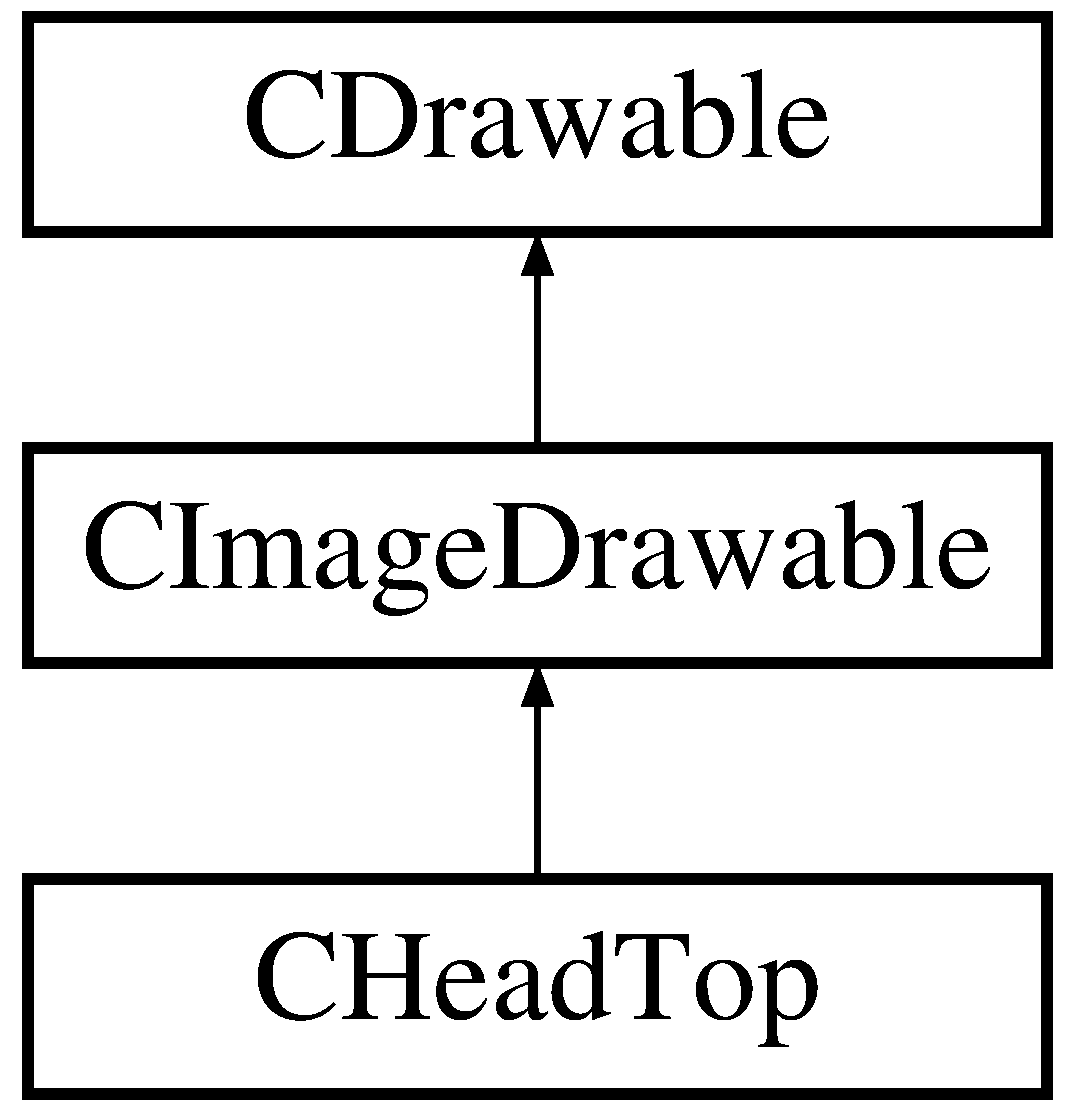
\includegraphics[height=3.000000cm]{class_c_image_drawable}
\end{center}
\end{figure}
\subsection*{Public Member Functions}
\begin{DoxyCompactItemize}
\item 
\hyperlink{class_c_image_drawable_a0af067ad80ece0bea046dded19c5b9d4}{C\+Image\+Drawable} ()=delete
\begin{DoxyCompactList}\small\item\em Default constructor disabled. \end{DoxyCompactList}\item 
\hypertarget{class_c_image_drawable_a2955356238c638373d39ed99c5422cf3}{\hyperlink{class_c_image_drawable_a2955356238c638373d39ed99c5422cf3}{C\+Image\+Drawable} (const \hyperlink{class_c_image_drawable}{C\+Image\+Drawable} \&)=delete}\label{class_c_image_drawable_a2955356238c638373d39ed99c5422cf3}

\begin{DoxyCompactList}\small\item\em Copy constructor disabled. \end{DoxyCompactList}\item 
\hypertarget{class_c_image_drawable_a717129f6ce9e9fa5d9a512a85a33a8b1}{void \hyperlink{class_c_image_drawable_a717129f6ce9e9fa5d9a512a85a33a8b1}{operator=} (const \hyperlink{class_c_image_drawable}{C\+Image\+Drawable} \&)=delete}\label{class_c_image_drawable_a717129f6ce9e9fa5d9a512a85a33a8b1}

\begin{DoxyCompactList}\small\item\em Assignment operator disabled. \end{DoxyCompactList}\item 
virtual \hyperlink{class_c_image_drawable_a4ecb6e494ba125a2d503bfff1260c2fe}{$\sim$\+C\+Image\+Drawable} ()
\begin{DoxyCompactList}\small\item\em Destructor. \end{DoxyCompactList}\item 
\hyperlink{class_c_image_drawable_a69a49fde766e126ad7b04aa2b6231d5e}{C\+Image\+Drawable} (const wstring \&name, const wstring \&filename)
\begin{DoxyCompactList}\small\item\em Constructor. \end{DoxyCompactList}\item 
void \hyperlink{class_c_image_drawable_a802c0e4223c536bf86f882ed75db1394}{Draw} (Graphics $\ast$graphics)
\begin{DoxyCompactList}\small\item\em Draws our image. \end{DoxyCompactList}\item 
bool \hyperlink{class_c_image_drawable_ae3093502b7858e397ee98b6366995356}{Hit\+Test} (Point pos)
\begin{DoxyCompactList}\small\item\em A hit-\/test for our image. \end{DoxyCompactList}\item 
Point \hyperlink{class_c_image_drawable_ab50ceb11d0002f4f8ffe5083006d317b}{Get\+Center} () const 
\begin{DoxyCompactList}\small\item\em Gets the center of our image. \end{DoxyCompactList}\item 
\hypertarget{class_c_image_drawable_a8de5ad7b65c518835989c7fe8b45af3d}{void \hyperlink{class_c_image_drawable_a8de5ad7b65c518835989c7fe8b45af3d}{Set\+Center} (Point center)}\label{class_c_image_drawable_a8de5ad7b65c518835989c7fe8b45af3d}

\begin{DoxyCompactList}\small\item\em Sets the center location  The point to set the center to. \end{DoxyCompactList}\end{DoxyCompactItemize}
\subsection*{Protected Attributes}
\begin{DoxyCompactItemize}
\item 
\hypertarget{class_c_image_drawable_ae55a012a4867007fc409db9d71476c71}{std\+::unique\+\_\+ptr$<$ Gdiplus\+::\+Bitmap $>$ \hyperlink{class_c_image_drawable_ae55a012a4867007fc409db9d71476c71}{m\+Image}}\label{class_c_image_drawable_ae55a012a4867007fc409db9d71476c71}

\begin{DoxyCompactList}\small\item\em The image for this drawable. \end{DoxyCompactList}\end{DoxyCompactItemize}
\subsection*{Additional Inherited Members}


\subsection{Detailed Description}
Class representing an image drawable (not polygon) 

\subsection{Constructor \& Destructor Documentation}
\hypertarget{class_c_image_drawable_a0af067ad80ece0bea046dded19c5b9d4}{\index{C\+Image\+Drawable@{C\+Image\+Drawable}!C\+Image\+Drawable@{C\+Image\+Drawable}}
\index{C\+Image\+Drawable@{C\+Image\+Drawable}!C\+Image\+Drawable@{C\+Image\+Drawable}}
\subsubsection[{C\+Image\+Drawable}]{\setlength{\rightskip}{0pt plus 5cm}C\+Image\+Drawable\+::\+C\+Image\+Drawable (
\begin{DoxyParamCaption}
{}
\end{DoxyParamCaption}
)\hspace{0.3cm}{\ttfamily [delete]}}}\label{class_c_image_drawable_a0af067ad80ece0bea046dded19c5b9d4}


Default constructor disabled. 

Remove Default, Copy, Assignment \hypertarget{class_c_image_drawable_a4ecb6e494ba125a2d503bfff1260c2fe}{\index{C\+Image\+Drawable@{C\+Image\+Drawable}!````~C\+Image\+Drawable@{$\sim$\+C\+Image\+Drawable}}
\index{````~C\+Image\+Drawable@{$\sim$\+C\+Image\+Drawable}!C\+Image\+Drawable@{C\+Image\+Drawable}}
\subsubsection[{$\sim$\+C\+Image\+Drawable}]{\setlength{\rightskip}{0pt plus 5cm}C\+Image\+Drawable\+::$\sim$\+C\+Image\+Drawable (
\begin{DoxyParamCaption}
{}
\end{DoxyParamCaption}
)\hspace{0.3cm}{\ttfamily [virtual]}}}\label{class_c_image_drawable_a4ecb6e494ba125a2d503bfff1260c2fe}


Destructor. 

Constructor \& Destructor \hypertarget{class_c_image_drawable_a69a49fde766e126ad7b04aa2b6231d5e}{\index{C\+Image\+Drawable@{C\+Image\+Drawable}!C\+Image\+Drawable@{C\+Image\+Drawable}}
\index{C\+Image\+Drawable@{C\+Image\+Drawable}!C\+Image\+Drawable@{C\+Image\+Drawable}}
\subsubsection[{C\+Image\+Drawable}]{\setlength{\rightskip}{0pt plus 5cm}C\+Image\+Drawable\+::\+C\+Image\+Drawable (
\begin{DoxyParamCaption}
\item[{const wstring \&}]{name, }
\item[{const wstring \&}]{filename}
\end{DoxyParamCaption}
)}}\label{class_c_image_drawable_a69a49fde766e126ad7b04aa2b6231d5e}


Constructor. 


\begin{DoxyParams}{Parameters}
{\em name} & -\/ A string to name our image by \\
\hline
{\em filename} & -\/ The filename of our image\\
\hline
{\em name} & The drawable name \\
\hline
{\em filename} & The filename for the image \\
\hline
\end{DoxyParams}


\subsection{Member Function Documentation}
\hypertarget{class_c_image_drawable_a802c0e4223c536bf86f882ed75db1394}{\index{C\+Image\+Drawable@{C\+Image\+Drawable}!Draw@{Draw}}
\index{Draw@{Draw}!C\+Image\+Drawable@{C\+Image\+Drawable}}
\subsubsection[{Draw}]{\setlength{\rightskip}{0pt plus 5cm}void C\+Image\+Drawable\+::\+Draw (
\begin{DoxyParamCaption}
\item[{Graphics $\ast$}]{graphics}
\end{DoxyParamCaption}
)}}\label{class_c_image_drawable_a802c0e4223c536bf86f882ed75db1394}


Draws our image. 

Draw the image drawable.

General Functions
\begin{DoxyParams}{Parameters}
{\em graphics} & -\/ The graphics context to draw our image on\\
\hline
{\em graphics} & Graphics context to draw on \\
\hline
\end{DoxyParams}
\hypertarget{class_c_image_drawable_ab50ceb11d0002f4f8ffe5083006d317b}{\index{C\+Image\+Drawable@{C\+Image\+Drawable}!Get\+Center@{Get\+Center}}
\index{Get\+Center@{Get\+Center}!C\+Image\+Drawable@{C\+Image\+Drawable}}
\subsubsection[{Get\+Center}]{\setlength{\rightskip}{0pt plus 5cm}Point C\+Image\+Drawable\+::\+Get\+Center (
\begin{DoxyParamCaption}
{}
\end{DoxyParamCaption}
) const\hspace{0.3cm}{\ttfamily [inline]}}}\label{class_c_image_drawable_ab50ceb11d0002f4f8ffe5083006d317b}


Gets the center of our image. 

Getters \& Setters\begin{DoxyReturn}{Returns}
Gdiplus\+::\+Point where the center of our image is 
\end{DoxyReturn}
\hypertarget{class_c_image_drawable_ae3093502b7858e397ee98b6366995356}{\index{C\+Image\+Drawable@{C\+Image\+Drawable}!Hit\+Test@{Hit\+Test}}
\index{Hit\+Test@{Hit\+Test}!C\+Image\+Drawable@{C\+Image\+Drawable}}
\subsubsection[{Hit\+Test}]{\setlength{\rightskip}{0pt plus 5cm}bool C\+Image\+Drawable\+::\+Hit\+Test (
\begin{DoxyParamCaption}
\item[{Point}]{pos}
\end{DoxyParamCaption}
)}}\label{class_c_image_drawable_ae3093502b7858e397ee98b6366995356}


A hit-\/test for our image. 

Test to see if we clicked on the image.


\begin{DoxyParams}{Parameters}
{\em pos} & -\/ A point to test for hitting \\
\hline
\end{DoxyParams}
\begin{DoxyReturn}{Returns}
True if we hit something at coordinates
\end{DoxyReturn}

\begin{DoxyParams}{Parameters}
{\em pos} & Position to test \\
\hline
\end{DoxyParams}
\begin{DoxyReturn}{Returns}
True if clicked on 
\end{DoxyReturn}


The documentation for this class was generated from the following files\+:\begin{DoxyCompactItemize}
\item 
\hyperlink{_image_drawable_8h}{Image\+Drawable.\+h}\item 
\hyperlink{_image_drawable_8cpp}{Image\+Drawable.\+cpp}\end{DoxyCompactItemize}

\hypertarget{class_c_main_frame}{\section{C\+Main\+Frame Class Reference}
\label{class_c_main_frame}\index{C\+Main\+Frame@{C\+Main\+Frame}}
}


Program main frame.  




{\ttfamily \#include $<$Main\+Frm.\+h$>$}

Inheritance diagram for C\+Main\+Frame\+:\begin{figure}[H]
\begin{center}
\leavevmode
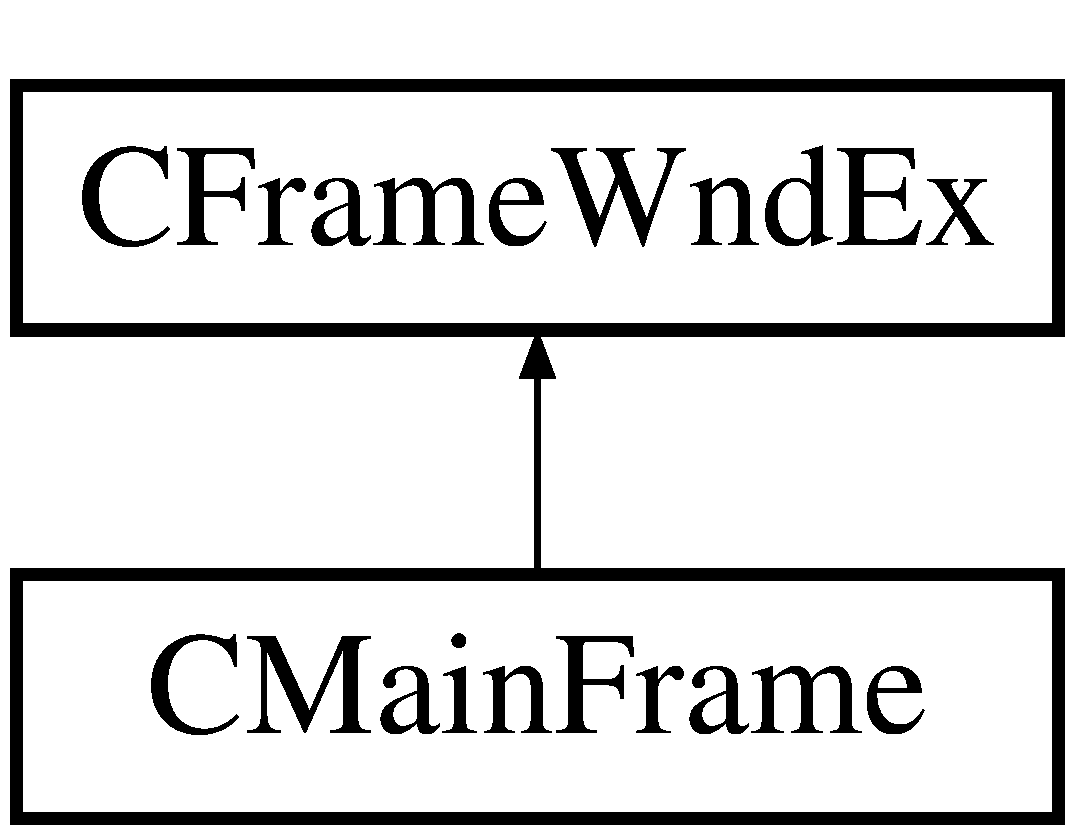
\includegraphics[height=2.000000cm]{class_c_main_frame}
\end{center}
\end{figure}
\subsection*{Public Types}
\begin{DoxyCompactItemize}
\item 
\hypertarget{class_c_main_frame_a89722c82d82f95a761772a8dd9755b7b}{enum \hyperlink{class_c_main_frame_a89722c82d82f95a761772a8dd9755b7b}{Motion\+Modes} \{ {\bfseries Move}, 
{\bfseries Rotate}
 \}}\label{class_c_main_frame_a89722c82d82f95a761772a8dd9755b7b}

\begin{DoxyCompactList}\small\item\em Enumerations for the possible manipulation modes. \end{DoxyCompactList}\end{DoxyCompactItemize}
\subsection*{Public Member Functions}
\begin{DoxyCompactItemize}
\item 
\hypertarget{class_c_main_frame_af3e997aeae4148d2aaa4a1e1ae7bdd53}{\hyperlink{class_c_main_frame_af3e997aeae4148d2aaa4a1e1ae7bdd53}{C\+Main\+Frame} ()}\label{class_c_main_frame_af3e997aeae4148d2aaa4a1e1ae7bdd53}

\begin{DoxyCompactList}\small\item\em Constructor. \end{DoxyCompactList}\item 
\hyperlink{class_c_main_frame_a89722c82d82f95a761772a8dd9755b7b}{Motion\+Modes} \hyperlink{class_c_main_frame_a76c571ab75752dba8049e08f5e4ac920}{Get\+Mode} () const 
\begin{DoxyCompactList}\small\item\em The selected manipulation mode. \end{DoxyCompactList}\item 
\hypertarget{class_c_main_frame_a549bf677c955c2898c3c683321633c16}{virtual B\+O\+O\+L {\bfseries Pre\+Create\+Window} (C\+R\+E\+A\+T\+E\+S\+T\+R\+U\+C\+T \&cs)}\label{class_c_main_frame_a549bf677c955c2898c3c683321633c16}

\item 
\hypertarget{class_c_main_frame_ade959eb0bab719bf06bb9b18ee407101}{virtual B\+O\+O\+L {\bfseries On\+Cmd\+Msg} (U\+I\+N\+T n\+I\+D, int n\+Code, void $\ast$p\+Extra, A\+F\+X\+\_\+\+C\+M\+D\+H\+A\+N\+D\+L\+E\+R\+I\+N\+F\+O $\ast$p\+Handler\+Info)}\label{class_c_main_frame_ade959eb0bab719bf06bb9b18ee407101}

\item 
\hypertarget{class_c_main_frame_a8ae555f23fdf97edb4feb4d3e1bfa4ee}{virtual \hyperlink{class_c_main_frame_a8ae555f23fdf97edb4feb4d3e1bfa4ee}{$\sim$\+C\+Main\+Frame} ()}\label{class_c_main_frame_a8ae555f23fdf97edb4feb4d3e1bfa4ee}

\begin{DoxyCompactList}\small\item\em Destructor. \end{DoxyCompactList}\item 
afx\+\_\+msg void \hyperlink{class_c_main_frame_adf171bf1f2c6f10cc85dbe8db3fc93f7}{On\+Size} (U\+I\+N\+T n\+Type, int cx, int cy)
\begin{DoxyCompactList}\small\item\em Handle a Size request from Windows. \end{DoxyCompactList}\item 
afx\+\_\+msg B\+O\+O\+L \hyperlink{class_c_main_frame_a53a97f2229c5765329b2b59a21a54b0d}{On\+Erase\+Bkgnd} (C\+D\+C $\ast$p\+D\+C)
\begin{DoxyCompactList}\small\item\em Called to erase the background. Disabled so we don't get flicker. \end{DoxyCompactList}\item 
\hypertarget{class_c_main_frame_af07c2610f9f5631e7eb7374d10d5fdd3}{afx\+\_\+msg void \hyperlink{class_c_main_frame_af07c2610f9f5631e7eb7374d10d5fdd3}{On\+Edit\+Move} ()}\label{class_c_main_frame_af07c2610f9f5631e7eb7374d10d5fdd3}

\begin{DoxyCompactList}\small\item\em Handle the Edit$>$Mode menu option. \end{DoxyCompactList}\item 
afx\+\_\+msg void \hyperlink{class_c_main_frame_aadc40c4ab290da2368f6b87443f5ffbc}{On\+Update\+Edit\+Move} (C\+Cmd\+U\+I $\ast$p\+Cmd\+U\+I)
\begin{DoxyCompactList}\small\item\em Update the menu for Edit$>$Move. \end{DoxyCompactList}\item 
\hypertarget{class_c_main_frame_a00f10667f35de1fa6693c1bea941d878}{afx\+\_\+msg void \hyperlink{class_c_main_frame_a00f10667f35de1fa6693c1bea941d878}{On\+Edit\+Rotate} ()}\label{class_c_main_frame_a00f10667f35de1fa6693c1bea941d878}

\begin{DoxyCompactList}\small\item\em Handle the Edit$>$Rotate menu option. \end{DoxyCompactList}\item 
afx\+\_\+msg void \hyperlink{class_c_main_frame_af098b8129775d1b5fb47fcaaabce8c01}{On\+Update\+Edit\+Rotate} (C\+Cmd\+U\+I $\ast$p\+Cmd\+U\+I)
\begin{DoxyCompactList}\small\item\em Update the menu for Edit$>$Rotate. \end{DoxyCompactList}\end{DoxyCompactItemize}
\subsection*{Protected Member Functions}
\begin{DoxyCompactItemize}
\item 
\hypertarget{class_c_main_frame_a48666466fd37412fcaeff75c3b12e0ed}{afx\+\_\+msg int {\bfseries On\+Create} (L\+P\+C\+R\+E\+A\+T\+E\+S\+T\+R\+U\+C\+T lp\+Create\+Struct)}\label{class_c_main_frame_a48666466fd37412fcaeff75c3b12e0ed}

\item 
\hypertarget{class_c_main_frame_adc353a3d1fc497fbc009b6d9e6914a82}{afx\+\_\+msg void {\bfseries On\+Set\+Focus} (C\+Wnd $\ast$p\+Old\+Wnd)}\label{class_c_main_frame_adc353a3d1fc497fbc009b6d9e6914a82}

\item 
\hypertarget{class_c_main_frame_ac863d694fd3637d492ef97396defbd8e}{virtual B\+O\+O\+L {\bfseries On\+Create\+Client} (L\+P\+C\+R\+E\+A\+T\+E\+S\+T\+R\+U\+C\+T lpcs, C\+Create\+Context $\ast$p\+Context)}\label{class_c_main_frame_ac863d694fd3637d492ef97396defbd8e}

\end{DoxyCompactItemize}
\subsection*{Protected Attributes}
\begin{DoxyCompactItemize}
\item 
\hypertarget{class_c_main_frame_ac8558942627d1502b5095e736840a1f3}{C\+M\+F\+C\+Tool\+Bar {\bfseries m\+\_\+wnd\+Tool\+Bar}}\label{class_c_main_frame_ac8558942627d1502b5095e736840a1f3}

\item 
\hypertarget{class_c_main_frame_a5842bded00e9137fbbf77343b99863be}{C\+M\+F\+C\+Status\+Bar {\bfseries m\+\_\+wnd\+Status\+Bar}}\label{class_c_main_frame_a5842bded00e9137fbbf77343b99863be}

\item 
\hypertarget{class_c_main_frame_a1d68466db594c4bebf41f707bc0a0647}{C\+Splitter\+Wnd {\bfseries m\+Wnd\+Splitter}}\label{class_c_main_frame_a1d68466db594c4bebf41f707bc0a0647}

\end{DoxyCompactItemize}


\subsection{Detailed Description}
Program main frame. 

\subsection{Member Function Documentation}
\hypertarget{class_c_main_frame_a76c571ab75752dba8049e08f5e4ac920}{\index{C\+Main\+Frame@{C\+Main\+Frame}!Get\+Mode@{Get\+Mode}}
\index{Get\+Mode@{Get\+Mode}!C\+Main\+Frame@{C\+Main\+Frame}}
\subsubsection[{Get\+Mode}]{\setlength{\rightskip}{0pt plus 5cm}{\bf Motion\+Modes} C\+Main\+Frame\+::\+Get\+Mode (
\begin{DoxyParamCaption}
{}
\end{DoxyParamCaption}
) const\hspace{0.3cm}{\ttfamily [inline]}}}\label{class_c_main_frame_a76c571ab75752dba8049e08f5e4ac920}


The selected manipulation mode. 

\begin{DoxyReturn}{Returns}
Currently selected manipulation mode 
\end{DoxyReturn}
\hypertarget{class_c_main_frame_a53a97f2229c5765329b2b59a21a54b0d}{\index{C\+Main\+Frame@{C\+Main\+Frame}!On\+Erase\+Bkgnd@{On\+Erase\+Bkgnd}}
\index{On\+Erase\+Bkgnd@{On\+Erase\+Bkgnd}!C\+Main\+Frame@{C\+Main\+Frame}}
\subsubsection[{On\+Erase\+Bkgnd}]{\setlength{\rightskip}{0pt plus 5cm}B\+O\+O\+L C\+Main\+Frame\+::\+On\+Erase\+Bkgnd (
\begin{DoxyParamCaption}
\item[{C\+D\+C $\ast$}]{p\+D\+C}
\end{DoxyParamCaption}
)}}\label{class_c_main_frame_a53a97f2229c5765329b2b59a21a54b0d}


Called to erase the background. Disabled so we don't get flicker. 


\begin{DoxyParams}{Parameters}
{\em p\+D\+C} & A device context \\
\hline
\end{DoxyParams}
\begin{DoxyReturn}{Returns}
F\+A\+L\+S\+E 
\end{DoxyReturn}
\hypertarget{class_c_main_frame_adf171bf1f2c6f10cc85dbe8db3fc93f7}{\index{C\+Main\+Frame@{C\+Main\+Frame}!On\+Size@{On\+Size}}
\index{On\+Size@{On\+Size}!C\+Main\+Frame@{C\+Main\+Frame}}
\subsubsection[{On\+Size}]{\setlength{\rightskip}{0pt plus 5cm}void C\+Main\+Frame\+::\+On\+Size (
\begin{DoxyParamCaption}
\item[{U\+I\+N\+T}]{n\+Type, }
\item[{int}]{cx, }
\item[{int}]{cy}
\end{DoxyParamCaption}
)}}\label{class_c_main_frame_adf171bf1f2c6f10cc85dbe8db3fc93f7}


Handle a Size request from Windows. 

This function ensures the child windows are the correct size on the screen after the main window is resized 
\begin{DoxyParams}{Parameters}
{\em n\+Type} & Type of resizing message \\
\hline
{\em cx} & The new width \\
\hline
{\em cy} & The new height \\
\hline
\end{DoxyParams}
\hypertarget{class_c_main_frame_aadc40c4ab290da2368f6b87443f5ffbc}{\index{C\+Main\+Frame@{C\+Main\+Frame}!On\+Update\+Edit\+Move@{On\+Update\+Edit\+Move}}
\index{On\+Update\+Edit\+Move@{On\+Update\+Edit\+Move}!C\+Main\+Frame@{C\+Main\+Frame}}
\subsubsection[{On\+Update\+Edit\+Move}]{\setlength{\rightskip}{0pt plus 5cm}void C\+Main\+Frame\+::\+On\+Update\+Edit\+Move (
\begin{DoxyParamCaption}
\item[{C\+Cmd\+U\+I $\ast$}]{p\+Cmd\+U\+I}
\end{DoxyParamCaption}
)}}\label{class_c_main_frame_aadc40c4ab290da2368f6b87443f5ffbc}


Update the menu for Edit$>$Move. 


\begin{DoxyParams}{Parameters}
{\em p\+Cmd\+U\+I} & The pointer to the control user interface \\
\hline
\end{DoxyParams}
\hypertarget{class_c_main_frame_af098b8129775d1b5fb47fcaaabce8c01}{\index{C\+Main\+Frame@{C\+Main\+Frame}!On\+Update\+Edit\+Rotate@{On\+Update\+Edit\+Rotate}}
\index{On\+Update\+Edit\+Rotate@{On\+Update\+Edit\+Rotate}!C\+Main\+Frame@{C\+Main\+Frame}}
\subsubsection[{On\+Update\+Edit\+Rotate}]{\setlength{\rightskip}{0pt plus 5cm}void C\+Main\+Frame\+::\+On\+Update\+Edit\+Rotate (
\begin{DoxyParamCaption}
\item[{C\+Cmd\+U\+I $\ast$}]{p\+Cmd\+U\+I}
\end{DoxyParamCaption}
)}}\label{class_c_main_frame_af098b8129775d1b5fb47fcaaabce8c01}


Update the menu for Edit$>$Rotate. 


\begin{DoxyParams}{Parameters}
{\em p\+Cmd\+U\+I} & The pointer to the control user interface \\
\hline
\end{DoxyParams}


The documentation for this class was generated from the following files\+:\begin{DoxyCompactItemize}
\item 
\hyperlink{_main_frm_8h}{Main\+Frm.\+h}\item 
\hyperlink{_main_frm_8cpp}{Main\+Frm.\+cpp}\end{DoxyCompactItemize}

\hypertarget{class_c_picture}{\section{C\+Picture Class Reference}
\label{class_c_picture}\index{C\+Picture@{C\+Picture}}
}


The picture we are drawing.  




{\ttfamily \#include $<$Picture.\+h$>$}

\subsection*{Classes}
\begin{DoxyCompactItemize}
\item 
class \hyperlink{class_c_picture_1_1_iter}{Iter}
\begin{DoxyCompactList}\small\item\em Iterator for iteration over actors in our picture. \end{DoxyCompactList}\end{DoxyCompactItemize}
\subsection*{Public Member Functions}
\begin{DoxyCompactItemize}
\item 
\hyperlink{class_c_picture_1_1_iter}{Iter} \hyperlink{class_c_picture_a5a4a9a34afcb8d8b6cbb337842292dcd}{begin} ()
\begin{DoxyCompactList}\small\item\em Get an iterator for the beginning of the collection. \end{DoxyCompactList}\item 
\hyperlink{class_c_picture_1_1_iter}{Iter} \hyperlink{class_c_picture_a49b85877b88711bd3e5dee27a439b16c}{end} ()
\begin{DoxyCompactList}\small\item\em Get an iterator for the end of the collection. \end{DoxyCompactList}\item 
\hyperlink{class_c_picture_a4e3783bef1f9d565b8a9f5e9680685ab}{C\+Picture} ()
\begin{DoxyCompactList}\small\item\em Constructor. \end{DoxyCompactList}\item 
virtual \hyperlink{class_c_picture_a763d6f41025f8e3f39c3ed264aac623c}{$\sim$\+C\+Picture} ()
\begin{DoxyCompactList}\small\item\em Virtual destructor. \end{DoxyCompactList}\item 
\hyperlink{class_c_picture_aa74c697e3bcca50430acbfa582f7a928}{C\+Picture} (const \hyperlink{class_c_picture}{C\+Picture} \&)=delete
\begin{DoxyCompactList}\small\item\em Copy Constructor (Disabled) \end{DoxyCompactList}\item 
\hypertarget{class_c_picture_a8b0fe5e8e17f415d010eedab79555b6e}{\hyperlink{class_c_picture}{C\+Picture} \& \hyperlink{class_c_picture_a8b0fe5e8e17f415d010eedab79555b6e}{operator=} (const \hyperlink{class_c_picture}{C\+Picture} \&)=delete}\label{class_c_picture_a8b0fe5e8e17f415d010eedab79555b6e}

\begin{DoxyCompactList}\small\item\em Assignment Operator (Disabled) \end{DoxyCompactList}\item 
Gdiplus\+::\+Size \hyperlink{class_c_picture_af2677c395a3cb8d6e7d0860839801e5b}{Get\+Size} ()
\begin{DoxyCompactList}\small\item\em The picture size. \end{DoxyCompactList}\item 
void \hyperlink{class_c_picture_a66b8de27d3435e19024307254e918e3a}{Set\+Size} (Gdiplus\+::\+Size size)
\begin{DoxyCompactList}\small\item\em The picture size. \end{DoxyCompactList}\item 
void \hyperlink{class_c_picture_a6be8632e9b1c468dcf27e8452baf5605}{Add\+Observer} (\hyperlink{class_c_picture_observer}{C\+Picture\+Observer} $\ast$observer)
\begin{DoxyCompactList}\small\item\em Adds an observer to this picture. \end{DoxyCompactList}\item 
void \hyperlink{class_c_picture_a548ad72979b2a11c2669d9896f32bf92}{Remove\+Observer} (\hyperlink{class_c_picture_observer}{C\+Picture\+Observer} $\ast$observer)
\begin{DoxyCompactList}\small\item\em Removes an observer to this picture. \end{DoxyCompactList}\item 
void \hyperlink{class_c_picture_a971ca9c9100725b7d1a900adcfe889d6}{Update\+Observers} ()
\begin{DoxyCompactList}\small\item\em Calls the update functions in each of the existing observers to tell the observers about what has changed in the picture. \end{DoxyCompactList}\item 
void \hyperlink{class_c_picture_aca6a4829388fdfe3ecdc42f0e788b712}{Draw} (Gdiplus\+::\+Graphics $\ast$graphics)
\begin{DoxyCompactList}\small\item\em Draws the picture with G\+D\+I. \end{DoxyCompactList}\item 
void \hyperlink{class_c_picture_af1afa6bacb63be5da88bd212a97c9931}{Add\+Actor} (shared\+\_\+ptr$<$ \hyperlink{class_c_actor}{C\+Actor} $>$ actor)
\begin{DoxyCompactList}\small\item\em Creates the association between a picture and adds an actor. \end{DoxyCompactList}\end{DoxyCompactItemize}


\subsection{Detailed Description}
The picture we are drawing. 

There will be one picture object that contains all of our actors, which then contains the drawables. 

\subsection{Constructor \& Destructor Documentation}
\hypertarget{class_c_picture_a4e3783bef1f9d565b8a9f5e9680685ab}{\index{C\+Picture@{C\+Picture}!C\+Picture@{C\+Picture}}
\index{C\+Picture@{C\+Picture}!C\+Picture@{C\+Picture}}
\subsubsection[{C\+Picture}]{\setlength{\rightskip}{0pt plus 5cm}C\+Picture\+::\+C\+Picture (
\begin{DoxyParamCaption}
{}
\end{DoxyParamCaption}
)}}\label{class_c_picture_a4e3783bef1f9d565b8a9f5e9680685ab}


Constructor. 

Constructor \& Destructor \hypertarget{class_c_picture_a763d6f41025f8e3f39c3ed264aac623c}{\index{C\+Picture@{C\+Picture}!````~C\+Picture@{$\sim$\+C\+Picture}}
\index{````~C\+Picture@{$\sim$\+C\+Picture}!C\+Picture@{C\+Picture}}
\subsubsection[{$\sim$\+C\+Picture}]{\setlength{\rightskip}{0pt plus 5cm}C\+Picture\+::$\sim$\+C\+Picture (
\begin{DoxyParamCaption}
{}
\end{DoxyParamCaption}
)\hspace{0.3cm}{\ttfamily [virtual]}}}\label{class_c_picture_a763d6f41025f8e3f39c3ed264aac623c}


Virtual destructor. 

Destructor. \hypertarget{class_c_picture_aa74c697e3bcca50430acbfa582f7a928}{\index{C\+Picture@{C\+Picture}!C\+Picture@{C\+Picture}}
\index{C\+Picture@{C\+Picture}!C\+Picture@{C\+Picture}}
\subsubsection[{C\+Picture}]{\setlength{\rightskip}{0pt plus 5cm}C\+Picture\+::\+C\+Picture (
\begin{DoxyParamCaption}
\item[{const {\bf C\+Picture} \&}]{}
\end{DoxyParamCaption}
)\hspace{0.3cm}{\ttfamily [delete]}}}\label{class_c_picture_aa74c697e3bcca50430acbfa582f7a928}


Copy Constructor (Disabled) 

Disabling 

\subsection{Member Function Documentation}
\hypertarget{class_c_picture_af1afa6bacb63be5da88bd212a97c9931}{\index{C\+Picture@{C\+Picture}!Add\+Actor@{Add\+Actor}}
\index{Add\+Actor@{Add\+Actor}!C\+Picture@{C\+Picture}}
\subsubsection[{Add\+Actor}]{\setlength{\rightskip}{0pt plus 5cm}void C\+Picture\+::\+Add\+Actor (
\begin{DoxyParamCaption}
\item[{shared\+\_\+ptr$<$ {\bf C\+Actor} $>$}]{actor}
\end{DoxyParamCaption}
)}}\label{class_c_picture_af1afa6bacb63be5da88bd212a97c9931}


Creates the association between a picture and adds an actor. 

Adds and actor to our picture.


\begin{DoxyParams}{Parameters}
{\em actor} & -\/ The actor to add\\
\hline
{\em actor} & -\/ The actor to add (create link) \\
\hline
\end{DoxyParams}
\hypertarget{class_c_picture_a6be8632e9b1c468dcf27e8452baf5605}{\index{C\+Picture@{C\+Picture}!Add\+Observer@{Add\+Observer}}
\index{Add\+Observer@{Add\+Observer}!C\+Picture@{C\+Picture}}
\subsubsection[{Add\+Observer}]{\setlength{\rightskip}{0pt plus 5cm}void C\+Picture\+::\+Add\+Observer (
\begin{DoxyParamCaption}
\item[{{\bf C\+Picture\+Observer} $\ast$}]{observer}
\end{DoxyParamCaption}
)}}\label{class_c_picture_a6be8632e9b1c468dcf27e8452baf5605}


Adds an observer to this picture. 

Add an observer to this picture.


\begin{DoxyParams}{Parameters}
{\em observer} & -\/ The observer to add\\
\hline
{\em observer} & The observer to add \\
\hline
\end{DoxyParams}
\hypertarget{class_c_picture_a5a4a9a34afcb8d8b6cbb337842292dcd}{\index{C\+Picture@{C\+Picture}!begin@{begin}}
\index{begin@{begin}!C\+Picture@{C\+Picture}}
\subsubsection[{begin}]{\setlength{\rightskip}{0pt plus 5cm}{\bf Iter} C\+Picture\+::begin (
\begin{DoxyParamCaption}
{}
\end{DoxyParamCaption}
)\hspace{0.3cm}{\ttfamily [inline]}}}\label{class_c_picture_a5a4a9a34afcb8d8b6cbb337842292dcd}


Get an iterator for the beginning of the collection. 

Iterator Implementation\begin{DoxyReturn}{Returns}
\hyperlink{class_c_picture_1_1_iter}{Iter} object at position 0 
\end{DoxyReturn}
\hypertarget{class_c_picture_aca6a4829388fdfe3ecdc42f0e788b712}{\index{C\+Picture@{C\+Picture}!Draw@{Draw}}
\index{Draw@{Draw}!C\+Picture@{C\+Picture}}
\subsubsection[{Draw}]{\setlength{\rightskip}{0pt plus 5cm}void C\+Picture\+::\+Draw (
\begin{DoxyParamCaption}
\item[{Gdiplus\+::\+Graphics $\ast$}]{graphics}
\end{DoxyParamCaption}
)}}\label{class_c_picture_aca6a4829388fdfe3ecdc42f0e788b712}


Draws the picture with G\+D\+I. 

Draws our picture.


\begin{DoxyParams}{Parameters}
{\em grahpics} & -\/ The device context to draw on\\
\hline
{\em graphics} & -\/ Our graphics context \\
\hline
\end{DoxyParams}
\hypertarget{class_c_picture_a49b85877b88711bd3e5dee27a439b16c}{\index{C\+Picture@{C\+Picture}!end@{end}}
\index{end@{end}!C\+Picture@{C\+Picture}}
\subsubsection[{end}]{\setlength{\rightskip}{0pt plus 5cm}{\bf Iter} C\+Picture\+::end (
\begin{DoxyParamCaption}
{}
\end{DoxyParamCaption}
)\hspace{0.3cm}{\ttfamily [inline]}}}\label{class_c_picture_a49b85877b88711bd3e5dee27a439b16c}


Get an iterator for the end of the collection. 

\begin{DoxyReturn}{Returns}
\hyperlink{class_c_picture_1_1_iter}{Iter} object at position past the end 
\end{DoxyReturn}
\hypertarget{class_c_picture_af2677c395a3cb8d6e7d0860839801e5b}{\index{C\+Picture@{C\+Picture}!Get\+Size@{Get\+Size}}
\index{Get\+Size@{Get\+Size}!C\+Picture@{C\+Picture}}
\subsubsection[{Get\+Size}]{\setlength{\rightskip}{0pt plus 5cm}Gdiplus\+::\+Size C\+Picture\+::\+Get\+Size (
\begin{DoxyParamCaption}
{}
\end{DoxyParamCaption}
)\hspace{0.3cm}{\ttfamily [inline]}}}\label{class_c_picture_af2677c395a3cb8d6e7d0860839801e5b}


The picture size. 

General Functions\begin{DoxyReturn}{Returns}
Size 
\end{DoxyReturn}
\hypertarget{class_c_picture_a548ad72979b2a11c2669d9896f32bf92}{\index{C\+Picture@{C\+Picture}!Remove\+Observer@{Remove\+Observer}}
\index{Remove\+Observer@{Remove\+Observer}!C\+Picture@{C\+Picture}}
\subsubsection[{Remove\+Observer}]{\setlength{\rightskip}{0pt plus 5cm}void C\+Picture\+::\+Remove\+Observer (
\begin{DoxyParamCaption}
\item[{{\bf C\+Picture\+Observer} $\ast$}]{observer}
\end{DoxyParamCaption}
)}}\label{class_c_picture_a548ad72979b2a11c2669d9896f32bf92}


Removes an observer to this picture. 

Remove an observer from this picture.


\begin{DoxyParams}{Parameters}
{\em observer} & -\/ The observer to remove\\
\hline
{\em observer} & The observer to remove \\
\hline
\end{DoxyParams}
\hypertarget{class_c_picture_a66b8de27d3435e19024307254e918e3a}{\index{C\+Picture@{C\+Picture}!Set\+Size@{Set\+Size}}
\index{Set\+Size@{Set\+Size}!C\+Picture@{C\+Picture}}
\subsubsection[{Set\+Size}]{\setlength{\rightskip}{0pt plus 5cm}void C\+Picture\+::\+Set\+Size (
\begin{DoxyParamCaption}
\item[{Gdiplus\+::\+Size}]{size}
\end{DoxyParamCaption}
)\hspace{0.3cm}{\ttfamily [inline]}}}\label{class_c_picture_a66b8de27d3435e19024307254e918e3a}


The picture size. 


\begin{DoxyParams}{Parameters}
{\em size} & The new picture size \\
\hline
\end{DoxyParams}
\hypertarget{class_c_picture_a971ca9c9100725b7d1a900adcfe889d6}{\index{C\+Picture@{C\+Picture}!Update\+Observers@{Update\+Observers}}
\index{Update\+Observers@{Update\+Observers}!C\+Picture@{C\+Picture}}
\subsubsection[{Update\+Observers}]{\setlength{\rightskip}{0pt plus 5cm}void C\+Picture\+::\+Update\+Observers (
\begin{DoxyParamCaption}
{}
\end{DoxyParamCaption}
)}}\label{class_c_picture_a971ca9c9100725b7d1a900adcfe889d6}


Calls the update functions in each of the existing observers to tell the observers about what has changed in the picture. 

Update all observers to indicate the picture has changed. 

The documentation for this class was generated from the following files\+:\begin{DoxyCompactItemize}
\item 
\hyperlink{_picture_8h}{Picture.\+h}\item 
\hyperlink{_picture_8cpp}{Picture.\+cpp}\end{DoxyCompactItemize}

\hypertarget{class_c_picture_factory}{\section{C\+Picture\+Factory Class Reference}
\label{class_c_picture_factory}\index{C\+Picture\+Factory@{C\+Picture\+Factory}}
}


A factory class that builds our picture.  




{\ttfamily \#include $<$Picture\+Factory.\+h$>$}

\subsection*{Public Member Functions}
\begin{DoxyCompactItemize}
\item 
\hypertarget{class_c_picture_factory_a70c077bc0e10a447b60b2a57c37fd982}{\hyperlink{class_c_picture_factory_a70c077bc0e10a447b60b2a57c37fd982}{C\+Picture\+Factory} ()}\label{class_c_picture_factory_a70c077bc0e10a447b60b2a57c37fd982}

\begin{DoxyCompactList}\small\item\em Constructor. \end{DoxyCompactList}\item 
\hypertarget{class_c_picture_factory_a3a5867e1e4757926826b71e1a6983764}{virtual \hyperlink{class_c_picture_factory_a3a5867e1e4757926826b71e1a6983764}{$\sim$\+C\+Picture\+Factory} ()}\label{class_c_picture_factory_a3a5867e1e4757926826b71e1a6983764}

\begin{DoxyCompactList}\small\item\em Destructor. \end{DoxyCompactList}\item 
shared\+\_\+ptr$<$ \hyperlink{class_c_picture}{C\+Picture} $>$ \hyperlink{class_c_picture_factory_a8510a417b59de544ce40715f8d790d08}{Create} ()
\begin{DoxyCompactList}\small\item\em Factory method to create a new picture. \end{DoxyCompactList}\end{DoxyCompactItemize}


\subsection{Detailed Description}
A factory class that builds our picture. 

\subsection{Member Function Documentation}
\hypertarget{class_c_picture_factory_a8510a417b59de544ce40715f8d790d08}{\index{C\+Picture\+Factory@{C\+Picture\+Factory}!Create@{Create}}
\index{Create@{Create}!C\+Picture\+Factory@{C\+Picture\+Factory}}
\subsubsection[{Create}]{\setlength{\rightskip}{0pt plus 5cm}std\+::shared\+\_\+ptr$<$ {\bf C\+Picture} $>$ C\+Picture\+Factory\+::\+Create (
\begin{DoxyParamCaption}
{}
\end{DoxyParamCaption}
)}}\label{class_c_picture_factory_a8510a417b59de544ce40715f8d790d08}


Factory method to create a new picture. 

\begin{DoxyReturn}{Returns}
The created picture

The created picture 
\end{DoxyReturn}
Adding Harold

Adding Butch 

The documentation for this class was generated from the following files\+:\begin{DoxyCompactItemize}
\item 
\hyperlink{_picture_factory_8h}{Picture\+Factory.\+h}\item 
\hyperlink{_picture_factory_8cpp}{Picture\+Factory.\+cpp}\end{DoxyCompactItemize}

\hypertarget{class_c_picture_observer}{\section{C\+Picture\+Observer Class Reference}
\label{class_c_picture_observer}\index{C\+Picture\+Observer@{C\+Picture\+Observer}}
}


Observer base class for a picture.  




{\ttfamily \#include $<$Picture\+Observer.\+h$>$}

Inheritance diagram for C\+Picture\+Observer\+:\begin{figure}[H]
\begin{center}
\leavevmode
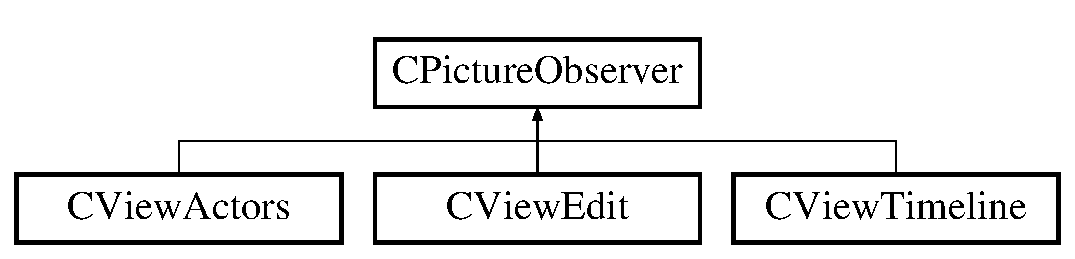
\includegraphics[height=2.000000cm]{class_c_picture_observer}
\end{center}
\end{figure}
\subsection*{Public Member Functions}
\begin{DoxyCompactItemize}
\item 
virtual \hyperlink{class_c_picture_observer_a86036f6ad66ae4bad3f204f61d234f46}{$\sim$\+C\+Picture\+Observer} ()
\begin{DoxyCompactList}\small\item\em Virtual destructor. \end{DoxyCompactList}\item 
\hypertarget{class_c_picture_observer_a7c0cae97a7c165b98a00aeb2892cd6e7}{\hyperlink{class_c_picture_observer_a7c0cae97a7c165b98a00aeb2892cd6e7}{C\+Picture\+Observer} (const \hyperlink{class_c_picture_observer}{C\+Picture\+Observer} \&)=delete}\label{class_c_picture_observer_a7c0cae97a7c165b98a00aeb2892cd6e7}

\begin{DoxyCompactList}\small\item\em Copy Constructor (Disabled) \end{DoxyCompactList}\item 
\hypertarget{class_c_picture_observer_a200c66fe9ab13e18e9559033165b1895}{\hyperlink{class_c_picture_observer}{C\+Picture\+Observer} \& \hyperlink{class_c_picture_observer_a200c66fe9ab13e18e9559033165b1895}{operator=} (const \hyperlink{class_c_picture_observer}{C\+Picture\+Observer} \&)=delete}\label{class_c_picture_observer_a200c66fe9ab13e18e9559033165b1895}

\begin{DoxyCompactList}\small\item\em Assignment Operator (Disabled) \end{DoxyCompactList}\item 
\hypertarget{class_c_picture_observer_a0dce27216a8cb8a2490f0efc83a5994a}{virtual void \hyperlink{class_c_picture_observer_a0dce27216a8cb8a2490f0efc83a5994a}{Update\+Observer} ()=0}\label{class_c_picture_observer_a0dce27216a8cb8a2490f0efc83a5994a}

\begin{DoxyCompactList}\small\item\em This function is called to update any observers. \end{DoxyCompactList}\item 
\hypertarget{class_c_picture_observer_ab7613c4badd101ace6a992b2eaaea153}{std\+::shared\+\_\+ptr$<$ \hyperlink{class_c_picture}{C\+Picture} $>$ \hyperlink{class_c_picture_observer_ab7613c4badd101ace6a992b2eaaea153}{Get\+Picture} ()}\label{class_c_picture_observer_ab7613c4badd101ace6a992b2eaaea153}

\begin{DoxyCompactList}\small\item\em Gets the picture we are observing. \end{DoxyCompactList}\item 
void \hyperlink{class_c_picture_observer_a8f4bd1a0d4e3b14b511d572a6dadeb7e}{Set\+Picture} (std\+::shared\+\_\+ptr$<$ \hyperlink{class_c_picture}{C\+Picture} $>$ picture)
\begin{DoxyCompactList}\small\item\em Sets the picture we are observing. \end{DoxyCompactList}\end{DoxyCompactItemize}
\subsection*{Protected Member Functions}
\begin{DoxyCompactItemize}
\item 
\hypertarget{class_c_picture_observer_a99e9a1639d81fcdb816921231fd10b99}{\hyperlink{class_c_picture_observer_a99e9a1639d81fcdb816921231fd10b99}{C\+Picture\+Observer} ()}\label{class_c_picture_observer_a99e9a1639d81fcdb816921231fd10b99}

\begin{DoxyCompactList}\small\item\em Constructor. \end{DoxyCompactList}\end{DoxyCompactItemize}


\subsection{Detailed Description}
Observer base class for a picture. 

This class implements the base class functionality for an observer in the observer pattern. 

\subsection{Constructor \& Destructor Documentation}
\hypertarget{class_c_picture_observer_a86036f6ad66ae4bad3f204f61d234f46}{\index{C\+Picture\+Observer@{C\+Picture\+Observer}!````~C\+Picture\+Observer@{$\sim$\+C\+Picture\+Observer}}
\index{````~C\+Picture\+Observer@{$\sim$\+C\+Picture\+Observer}!C\+Picture\+Observer@{C\+Picture\+Observer}}
\subsubsection[{$\sim$\+C\+Picture\+Observer}]{\setlength{\rightskip}{0pt plus 5cm}C\+Picture\+Observer\+::$\sim$\+C\+Picture\+Observer (
\begin{DoxyParamCaption}
{}
\end{DoxyParamCaption}
)\hspace{0.3cm}{\ttfamily [virtual]}}}\label{class_c_picture_observer_a86036f6ad66ae4bad3f204f61d234f46}


Virtual destructor. 

Destructor. 

\subsection{Member Function Documentation}
\hypertarget{class_c_picture_observer_a8f4bd1a0d4e3b14b511d572a6dadeb7e}{\index{C\+Picture\+Observer@{C\+Picture\+Observer}!Set\+Picture@{Set\+Picture}}
\index{Set\+Picture@{Set\+Picture}!C\+Picture\+Observer@{C\+Picture\+Observer}}
\subsubsection[{Set\+Picture}]{\setlength{\rightskip}{0pt plus 5cm}void C\+Picture\+Observer\+::\+Set\+Picture (
\begin{DoxyParamCaption}
\item[{std\+::shared\+\_\+ptr$<$ {\bf C\+Picture} $>$}]{picture}
\end{DoxyParamCaption}
)}}\label{class_c_picture_observer_a8f4bd1a0d4e3b14b511d572a6dadeb7e}


Sets the picture we are observing. 

Set the picture for this observer.


\begin{DoxyParams}{Parameters}
{\em picture} & The picture to set \\
\hline
\end{DoxyParams}


The documentation for this class was generated from the following files\+:\begin{DoxyCompactItemize}
\item 
\hyperlink{_picture_observer_8h}{Picture\+Observer.\+h}\item 
\hyperlink{_picture_observer_8cpp}{Picture\+Observer.\+cpp}\end{DoxyCompactItemize}

\hypertarget{class_c_poly_drawable}{\section{C\+Poly\+Drawable Class Reference}
\label{class_c_poly_drawable}\index{C\+Poly\+Drawable@{C\+Poly\+Drawable}}
}


A drawable based on polygon images.  




{\ttfamily \#include $<$Poly\+Drawable.\+h$>$}

Inheritance diagram for C\+Poly\+Drawable\+:\begin{figure}[H]
\begin{center}
\leavevmode
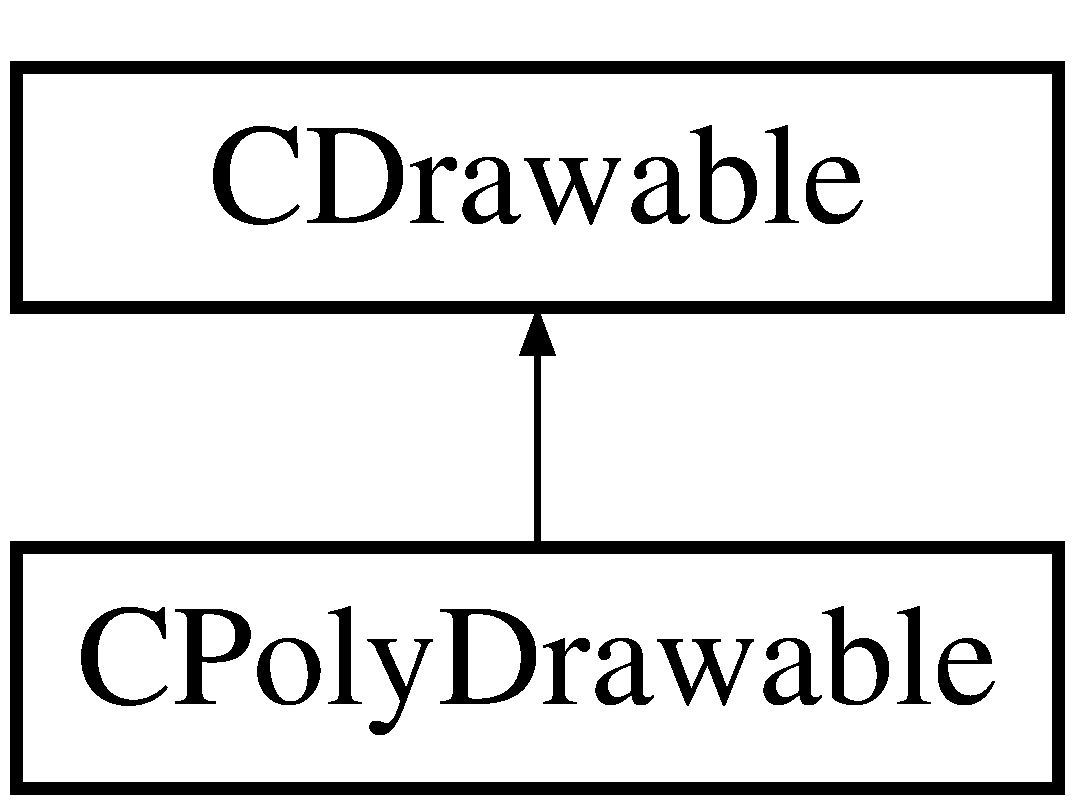
\includegraphics[height=2.000000cm]{class_c_poly_drawable}
\end{center}
\end{figure}
\subsection*{Public Member Functions}
\begin{DoxyCompactItemize}
\item 
\hyperlink{class_c_poly_drawable_ae4265afa898200aa70a943cdea3f8123}{C\+Poly\+Drawable} ()=delete
\begin{DoxyCompactList}\small\item\em Default constructor disabled. \end{DoxyCompactList}\item 
\hypertarget{class_c_poly_drawable_abfdd10484ab2cb6ea99c01849cad4082}{\hyperlink{class_c_poly_drawable_abfdd10484ab2cb6ea99c01849cad4082}{C\+Poly\+Drawable} (const \hyperlink{class_c_poly_drawable}{C\+Poly\+Drawable} \&)=delete}\label{class_c_poly_drawable_abfdd10484ab2cb6ea99c01849cad4082}

\begin{DoxyCompactList}\small\item\em Copy constructor disabled. \end{DoxyCompactList}\item 
\hypertarget{class_c_poly_drawable_a86a6c65081b7feb556e5563b36a6ac8a}{void \hyperlink{class_c_poly_drawable_a86a6c65081b7feb556e5563b36a6ac8a}{operator=} (const \hyperlink{class_c_poly_drawable}{C\+Poly\+Drawable} \&)=delete}\label{class_c_poly_drawable_a86a6c65081b7feb556e5563b36a6ac8a}

\begin{DoxyCompactList}\small\item\em Assignment operator disabled. \end{DoxyCompactList}\item 
\hyperlink{class_c_poly_drawable_acc013a0894a8f20fc29ae83af8d98c02}{C\+Poly\+Drawable} (const wstring \&name)
\begin{DoxyCompactList}\small\item\em Our non-\/default constructor. \end{DoxyCompactList}\item 
virtual \hyperlink{class_c_poly_drawable_afc766fdf8f37312434063b3b615f410b}{$\sim$\+C\+Poly\+Drawable} ()
\begin{DoxyCompactList}\small\item\em Virtual destructor. \end{DoxyCompactList}\item 
void \hyperlink{class_c_poly_drawable_acbc65a156643745e0279f16a5b872917}{Draw} (Graphics $\ast$graphics)
\begin{DoxyCompactList}\small\item\em Draws our polydrawable. \end{DoxyCompactList}\item 
bool \hyperlink{class_c_poly_drawable_a24b9ca4cf68fe5aa15d72ebb9e201607}{Hit\+Test} (Point pos)
\begin{DoxyCompactList}\small\item\em A hit test for our polydraw. \end{DoxyCompactList}\item 
void \hyperlink{class_c_poly_drawable_a2b4e35ccc929379c6611ca5c9c2f27d2}{Add\+Point} (Point point)
\begin{DoxyCompactList}\small\item\em Adds a point to our polydrawable. \end{DoxyCompactList}\item 
Color \hyperlink{class_c_poly_drawable_a80d95003679e105c5cc3ea44ba27a1a1}{Get\+Color} () const 
\begin{DoxyCompactList}\small\item\em Gets our poly color. \end{DoxyCompactList}\item 
\hypertarget{class_c_poly_drawable_ac10112aae056a96e760a13092b1edc96}{void \hyperlink{class_c_poly_drawable_ac10112aae056a96e760a13092b1edc96}{Set\+Color} (Color color)}\label{class_c_poly_drawable_ac10112aae056a96e760a13092b1edc96}

\begin{DoxyCompactList}\small\item\em Sets the color for our polydraw object  The Gdiplus\+::\+Color we wish to change it to. \end{DoxyCompactList}\end{DoxyCompactItemize}
\subsection*{Additional Inherited Members}


\subsection{Detailed Description}
A drawable based on polygon images. 

This class has a list of points and draws a polygon drawable based on those points. 

\subsection{Constructor \& Destructor Documentation}
\hypertarget{class_c_poly_drawable_ae4265afa898200aa70a943cdea3f8123}{\index{C\+Poly\+Drawable@{C\+Poly\+Drawable}!C\+Poly\+Drawable@{C\+Poly\+Drawable}}
\index{C\+Poly\+Drawable@{C\+Poly\+Drawable}!C\+Poly\+Drawable@{C\+Poly\+Drawable}}
\subsubsection[{C\+Poly\+Drawable}]{\setlength{\rightskip}{0pt plus 5cm}C\+Poly\+Drawable\+::\+C\+Poly\+Drawable (
\begin{DoxyParamCaption}
{}
\end{DoxyParamCaption}
)\hspace{0.3cm}{\ttfamily [delete]}}}\label{class_c_poly_drawable_ae4265afa898200aa70a943cdea3f8123}


Default constructor disabled. 

Disabling Default, Copy, Assignment \hypertarget{class_c_poly_drawable_acc013a0894a8f20fc29ae83af8d98c02}{\index{C\+Poly\+Drawable@{C\+Poly\+Drawable}!C\+Poly\+Drawable@{C\+Poly\+Drawable}}
\index{C\+Poly\+Drawable@{C\+Poly\+Drawable}!C\+Poly\+Drawable@{C\+Poly\+Drawable}}
\subsubsection[{C\+Poly\+Drawable}]{\setlength{\rightskip}{0pt plus 5cm}C\+Poly\+Drawable\+::\+C\+Poly\+Drawable (
\begin{DoxyParamCaption}
\item[{const wstring \&}]{name}
\end{DoxyParamCaption}
)}}\label{class_c_poly_drawable_acc013a0894a8f20fc29ae83af8d98c02}


Our non-\/default constructor. 

Constructor \& Destructor
\begin{DoxyParams}{Parameters}
{\em name} & -\/ The name to give our polydraw \\
\hline
\end{DoxyParams}
\hypertarget{class_c_poly_drawable_afc766fdf8f37312434063b3b615f410b}{\index{C\+Poly\+Drawable@{C\+Poly\+Drawable}!````~C\+Poly\+Drawable@{$\sim$\+C\+Poly\+Drawable}}
\index{````~C\+Poly\+Drawable@{$\sim$\+C\+Poly\+Drawable}!C\+Poly\+Drawable@{C\+Poly\+Drawable}}
\subsubsection[{$\sim$\+C\+Poly\+Drawable}]{\setlength{\rightskip}{0pt plus 5cm}C\+Poly\+Drawable\+::$\sim$\+C\+Poly\+Drawable (
\begin{DoxyParamCaption}
{}
\end{DoxyParamCaption}
)\hspace{0.3cm}{\ttfamily [virtual]}}}\label{class_c_poly_drawable_afc766fdf8f37312434063b3b615f410b}


Virtual destructor. 

Destructor. 

\subsection{Member Function Documentation}
\hypertarget{class_c_poly_drawable_a2b4e35ccc929379c6611ca5c9c2f27d2}{\index{C\+Poly\+Drawable@{C\+Poly\+Drawable}!Add\+Point@{Add\+Point}}
\index{Add\+Point@{Add\+Point}!C\+Poly\+Drawable@{C\+Poly\+Drawable}}
\subsubsection[{Add\+Point}]{\setlength{\rightskip}{0pt plus 5cm}void C\+Poly\+Drawable\+::\+Add\+Point (
\begin{DoxyParamCaption}
\item[{Point}]{point}
\end{DoxyParamCaption}
)}}\label{class_c_poly_drawable_a2b4e35ccc929379c6611ca5c9c2f27d2}


Adds a point to our polydrawable. 


\begin{DoxyParams}{Parameters}
{\em point} & -\/ The point to add \\
\hline
\end{DoxyParams}
\hypertarget{class_c_poly_drawable_acbc65a156643745e0279f16a5b872917}{\index{C\+Poly\+Drawable@{C\+Poly\+Drawable}!Draw@{Draw}}
\index{Draw@{Draw}!C\+Poly\+Drawable@{C\+Poly\+Drawable}}
\subsubsection[{Draw}]{\setlength{\rightskip}{0pt plus 5cm}void C\+Poly\+Drawable\+::\+Draw (
\begin{DoxyParamCaption}
\item[{Graphics $\ast$}]{graphics}
\end{DoxyParamCaption}
)}}\label{class_c_poly_drawable_acbc65a156643745e0279f16a5b872917}


Draws our polydrawable. 

Draw our polygon.

General Functions
\begin{DoxyParams}{Parameters}
{\em graphics} & -\/ the graphics to draw to\\
\hline
{\em graphics} & The graphics context to draw on \\
\hline
\end{DoxyParams}
\hypertarget{class_c_poly_drawable_a80d95003679e105c5cc3ea44ba27a1a1}{\index{C\+Poly\+Drawable@{C\+Poly\+Drawable}!Get\+Color@{Get\+Color}}
\index{Get\+Color@{Get\+Color}!C\+Poly\+Drawable@{C\+Poly\+Drawable}}
\subsubsection[{Get\+Color}]{\setlength{\rightskip}{0pt plus 5cm}Color C\+Poly\+Drawable\+::\+Get\+Color (
\begin{DoxyParamCaption}
{}
\end{DoxyParamCaption}
) const\hspace{0.3cm}{\ttfamily [inline]}}}\label{class_c_poly_drawable_a80d95003679e105c5cc3ea44ba27a1a1}


Gets our poly color. 

Getters \& Setters\begin{DoxyReturn}{Returns}
Gdiplus\+::\+Color representing our polydraw color 
\end{DoxyReturn}
\hypertarget{class_c_poly_drawable_a24b9ca4cf68fe5aa15d72ebb9e201607}{\index{C\+Poly\+Drawable@{C\+Poly\+Drawable}!Hit\+Test@{Hit\+Test}}
\index{Hit\+Test@{Hit\+Test}!C\+Poly\+Drawable@{C\+Poly\+Drawable}}
\subsubsection[{Hit\+Test}]{\setlength{\rightskip}{0pt plus 5cm}bool C\+Poly\+Drawable\+::\+Hit\+Test (
\begin{DoxyParamCaption}
\item[{Point}]{pos}
\end{DoxyParamCaption}
)}}\label{class_c_poly_drawable_a24b9ca4cf68fe5aa15d72ebb9e201607}


A hit test for our polydraw. 

Test to see if we hit this object with a mouse click.


\begin{DoxyParams}{Parameters}
{\em pos} & -\/ The point to hit test \\
\hline
\end{DoxyParams}
\begin{DoxyReturn}{Returns}
A boolean of true if we hit something
\end{DoxyReturn}

\begin{DoxyParams}{Parameters}
{\em pos} & Click position \\
\hline
\end{DoxyParams}
\begin{DoxyReturn}{Returns}
true it hit 
\end{DoxyReturn}


The documentation for this class was generated from the following files\+:\begin{DoxyCompactItemize}
\item 
\hyperlink{_poly_drawable_8h}{Poly\+Drawable.\+h}\item 
\hyperlink{_poly_drawable_8cpp}{Poly\+Drawable.\+cpp}\end{DoxyCompactItemize}

\hypertarget{class_c_view_actors}{\section{C\+View\+Actors Class Reference}
\label{class_c_view_actors}\index{C\+View\+Actors@{C\+View\+Actors}}
}


Class that provides a view windows for actors.  




{\ttfamily \#include $<$View\+Actors.\+h$>$}

Inheritance diagram for C\+View\+Actors\+:\begin{figure}[H]
\begin{center}
\leavevmode
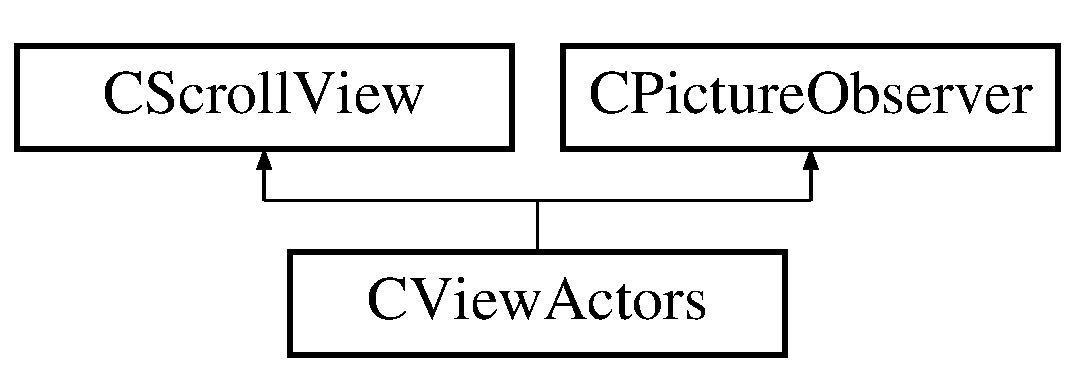
\includegraphics[height=2.000000cm]{class_c_view_actors}
\end{center}
\end{figure}
\subsection*{Public Member Functions}
\begin{DoxyCompactItemize}
\item 
void \hyperlink{class_c_view_actors_a6f68ae9e71f6a195502464bf34b3e724}{Set\+Main\+Frame} (\hyperlink{class_c_main_frame}{C\+Main\+Frame} $\ast$main\+Frame)
\begin{DoxyCompactList}\small\item\em Set the main\+Frame pointer. \end{DoxyCompactList}\item 
virtual void \hyperlink{class_c_view_actors_a5014f8c616850b8e874dee895b2ba698}{Update\+Observer} () override
\begin{DoxyCompactList}\small\item\em Updates the observer. \end{DoxyCompactList}\item 
afx\+\_\+msg B\+O\+O\+L \hyperlink{class_c_view_actors_a561f4be212bd5df4a667c2cb0b23e472}{On\+Erase\+Bkgnd} (C\+D\+C $\ast$p\+D\+C)
\begin{DoxyCompactList}\small\item\em Erase the background. \end{DoxyCompactList}\end{DoxyCompactItemize}
\subsection*{Static Public Attributes}
\begin{DoxyCompactItemize}
\item 
\hypertarget{class_c_view_actors_a8bb27cbe8ae099abbed012adca884f1f}{static const int \hyperlink{class_c_view_actors_a8bb27cbe8ae099abbed012adca884f1f}{Width} = 150}\label{class_c_view_actors_a8bb27cbe8ae099abbed012adca884f1f}

\begin{DoxyCompactList}\small\item\em Width we want for this window. \end{DoxyCompactList}\end{DoxyCompactItemize}
\subsection*{Protected Member Functions}
\begin{DoxyCompactItemize}
\item 
\hyperlink{class_c_view_actors_aeff00d958ecea52760ec07c0420c4e28}{C\+View\+Actors} ()
\begin{DoxyCompactList}\small\item\em $\ast$/ \end{DoxyCompactList}\item 
\hypertarget{class_c_view_actors_a6e1aa1c82708dd805ac90c21b6d521e0}{virtual \hyperlink{class_c_view_actors_a6e1aa1c82708dd805ac90c21b6d521e0}{$\sim$\+C\+View\+Actors} ()}\label{class_c_view_actors_a6e1aa1c82708dd805ac90c21b6d521e0}

\begin{DoxyCompactList}\small\item\em Destructor. \end{DoxyCompactList}\item 
virtual void \hyperlink{class_c_view_actors_aa68465c2f13e487426508832a6355503}{On\+Draw} (C\+D\+C $\ast$p\+D\+C)
\begin{DoxyCompactList}\small\item\em Draw this window. \end{DoxyCompactList}\item 
\hypertarget{class_c_view_actors_aaf83b3647a42330c01be9067a6235d33}{virtual void \hyperlink{class_c_view_actors_aaf83b3647a42330c01be9067a6235d33}{On\+Initial\+Update} ()}\label{class_c_view_actors_aaf83b3647a42330c01be9067a6235d33}

\begin{DoxyCompactList}\small\item\em Handle the initial update for this window. \end{DoxyCompactList}\end{DoxyCompactItemize}


\subsection{Detailed Description}
Class that provides a view windows for actors. 

\subsection{Constructor \& Destructor Documentation}
\hypertarget{class_c_view_actors_aeff00d958ecea52760ec07c0420c4e28}{\index{C\+View\+Actors@{C\+View\+Actors}!C\+View\+Actors@{C\+View\+Actors}}
\index{C\+View\+Actors@{C\+View\+Actors}!C\+View\+Actors@{C\+View\+Actors}}
\subsubsection[{C\+View\+Actors}]{\setlength{\rightskip}{0pt plus 5cm}C\+View\+Actors\+::\+C\+View\+Actors (
\begin{DoxyParamCaption}
{}
\end{DoxyParamCaption}
)\hspace{0.3cm}{\ttfamily [protected]}}}\label{class_c_view_actors_aeff00d958ecea52760ec07c0420c4e28}


$\ast$/ 

Constructor 

\subsection{Member Function Documentation}
\hypertarget{class_c_view_actors_aa68465c2f13e487426508832a6355503}{\index{C\+View\+Actors@{C\+View\+Actors}!On\+Draw@{On\+Draw}}
\index{On\+Draw@{On\+Draw}!C\+View\+Actors@{C\+View\+Actors}}
\subsubsection[{On\+Draw}]{\setlength{\rightskip}{0pt plus 5cm}void C\+View\+Actors\+::\+On\+Draw (
\begin{DoxyParamCaption}
\item[{C\+D\+C $\ast$}]{p\+D\+C}
\end{DoxyParamCaption}
)\hspace{0.3cm}{\ttfamily [protected]}, {\ttfamily [virtual]}}}\label{class_c_view_actors_aa68465c2f13e487426508832a6355503}


Draw this window. 


\begin{DoxyParams}{Parameters}
{\em p\+D\+C} & Device context \\
\hline
\end{DoxyParams}
\hypertarget{class_c_view_actors_a561f4be212bd5df4a667c2cb0b23e472}{\index{C\+View\+Actors@{C\+View\+Actors}!On\+Erase\+Bkgnd@{On\+Erase\+Bkgnd}}
\index{On\+Erase\+Bkgnd@{On\+Erase\+Bkgnd}!C\+View\+Actors@{C\+View\+Actors}}
\subsubsection[{On\+Erase\+Bkgnd}]{\setlength{\rightskip}{0pt plus 5cm}B\+O\+O\+L C\+View\+Actors\+::\+On\+Erase\+Bkgnd (
\begin{DoxyParamCaption}
\item[{C\+D\+C $\ast$}]{p\+D\+C}
\end{DoxyParamCaption}
)}}\label{class_c_view_actors_a561f4be212bd5df4a667c2cb0b23e472}


Erase the background. 

This is disabled to eliminate flicker 
\begin{DoxyParams}{Parameters}
{\em p\+D\+C} & Device context \\
\hline
\end{DoxyParams}
\begin{DoxyReturn}{Returns}
F\+A\+L\+S\+E 
\end{DoxyReturn}
\hypertarget{class_c_view_actors_a6f68ae9e71f6a195502464bf34b3e724}{\index{C\+View\+Actors@{C\+View\+Actors}!Set\+Main\+Frame@{Set\+Main\+Frame}}
\index{Set\+Main\+Frame@{Set\+Main\+Frame}!C\+View\+Actors@{C\+View\+Actors}}
\subsubsection[{Set\+Main\+Frame}]{\setlength{\rightskip}{0pt plus 5cm}void C\+View\+Actors\+::\+Set\+Main\+Frame (
\begin{DoxyParamCaption}
\item[{{\bf C\+Main\+Frame} $\ast$}]{main\+Frame}
\end{DoxyParamCaption}
)\hspace{0.3cm}{\ttfamily [inline]}}}\label{class_c_view_actors_a6f68ae9e71f6a195502464bf34b3e724}


Set the main\+Frame pointer. 


\begin{DoxyParams}{Parameters}
{\em main\+Frame} & Pointer to the \hyperlink{class_c_main_frame}{C\+Main\+Frame} window \\
\hline
\end{DoxyParams}
\hypertarget{class_c_view_actors_a5014f8c616850b8e874dee895b2ba698}{\index{C\+View\+Actors@{C\+View\+Actors}!Update\+Observer@{Update\+Observer}}
\index{Update\+Observer@{Update\+Observer}!C\+View\+Actors@{C\+View\+Actors}}
\subsubsection[{Update\+Observer}]{\setlength{\rightskip}{0pt plus 5cm}void C\+View\+Actors\+::\+Update\+Observer (
\begin{DoxyParamCaption}
{}
\end{DoxyParamCaption}
)\hspace{0.3cm}{\ttfamily [override]}, {\ttfamily [virtual]}}}\label{class_c_view_actors_a5014f8c616850b8e874dee895b2ba698}


Updates the observer. 

Force an update of this window when the picture changes. 

Implements \hyperlink{class_c_picture_observer_a0dce27216a8cb8a2490f0efc83a5994a}{C\+Picture\+Observer}.



The documentation for this class was generated from the following files\+:\begin{DoxyCompactItemize}
\item 
\hyperlink{_view_actors_8h}{View\+Actors.\+h}\item 
\hyperlink{_view_actors_8cpp}{View\+Actors.\+cpp}\end{DoxyCompactItemize}

\hypertarget{class_c_view_edit}{\section{C\+View\+Edit Class Reference}
\label{class_c_view_edit}\index{C\+View\+Edit@{C\+View\+Edit}}
}


View class the provides a window for editing our pixture.  




{\ttfamily \#include $<$View\+Edit.\+h$>$}

Inheritance diagram for C\+View\+Edit\+:\begin{figure}[H]
\begin{center}
\leavevmode
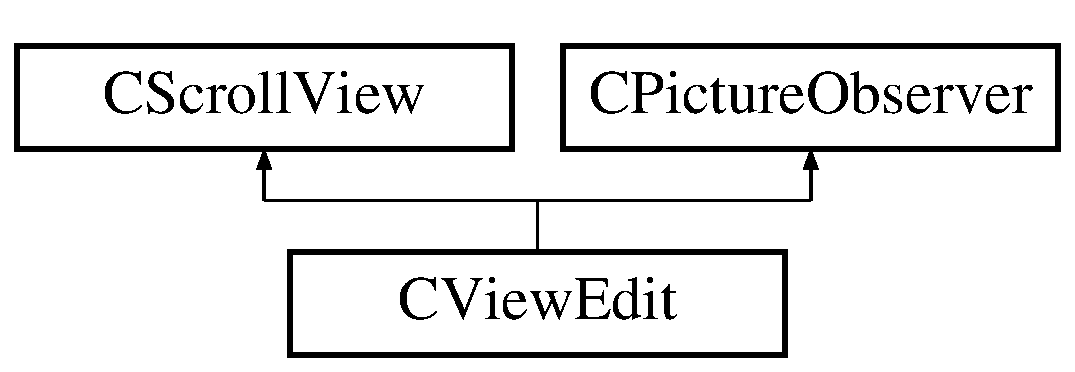
\includegraphics[height=2.000000cm]{class_c_view_edit}
\end{center}
\end{figure}
\subsection*{Public Member Functions}
\begin{DoxyCompactItemize}
\item 
\hypertarget{class_c_view_edit_a99fea37450207a1ffe8cf6b46ec2a11f}{\hyperlink{class_c_view_edit_a99fea37450207a1ffe8cf6b46ec2a11f}{C\+View\+Edit} ()}\label{class_c_view_edit_a99fea37450207a1ffe8cf6b46ec2a11f}

\begin{DoxyCompactList}\small\item\em Constructor. \end{DoxyCompactList}\item 
\hypertarget{class_c_view_edit_a968f16ef61489033c80ebe504017db3a}{virtual \hyperlink{class_c_view_edit_a968f16ef61489033c80ebe504017db3a}{$\sim$\+C\+View\+Edit} ()}\label{class_c_view_edit_a968f16ef61489033c80ebe504017db3a}

\begin{DoxyCompactList}\small\item\em Destructor. \end{DoxyCompactList}\item 
void \hyperlink{class_c_view_edit_a28bb793d43baba78e9b1c704b4f0e128}{Set\+Main\+Frame} (\hyperlink{class_c_main_frame}{C\+Main\+Frame} $\ast$main\+Frame)
\begin{DoxyCompactList}\small\item\em Set the main\+Frame pointer. \end{DoxyCompactList}\item 
\hypertarget{class_c_view_edit_ac2b73f20fe10a4a98096facde6450e5a}{virtual void \hyperlink{class_c_view_edit_ac2b73f20fe10a4a98096facde6450e5a}{Update\+Observer} () override}\label{class_c_view_edit_ac2b73f20fe10a4a98096facde6450e5a}

\begin{DoxyCompactList}\small\item\em Force an update of this window when the picture changes. \end{DoxyCompactList}\item 
afx\+\_\+msg B\+O\+O\+L \hyperlink{class_c_view_edit_a66446b22920245bb3b5c5735754d63cd}{On\+Erase\+Bkgnd} (C\+D\+C $\ast$p\+D\+C)
\begin{DoxyCompactList}\small\item\em Erase the background. \end{DoxyCompactList}\item 
afx\+\_\+msg void \hyperlink{class_c_view_edit_a0e77d59dd1ed299c933f660d9ff0cf7e}{On\+L\+Button\+Down} (U\+I\+N\+T n\+Flags, C\+Point point)
\begin{DoxyCompactList}\small\item\em Handle a left button click. \end{DoxyCompactList}\item 
afx\+\_\+msg void \hyperlink{class_c_view_edit_aba0b38ee4b51f9d98bc08ade92d9f051}{On\+Mouse\+Move} (U\+I\+N\+T n\+Flags, C\+Point point)
\begin{DoxyCompactList}\small\item\em Handle mouse movement. \end{DoxyCompactList}\end{DoxyCompactItemize}
\subsection*{Protected Member Functions}
\begin{DoxyCompactItemize}
\item 
virtual void \hyperlink{class_c_view_edit_a8cf50c2cebab5aaecda5ae6f7437cf38}{On\+Draw} (C\+D\+C $\ast$p\+D\+C)
\begin{DoxyCompactList}\small\item\em Drawing of the window. \end{DoxyCompactList}\item 
\hypertarget{class_c_view_edit_ac49ed2e9e35cd014c6539aaa4ac705f3}{virtual void \hyperlink{class_c_view_edit_ac49ed2e9e35cd014c6539aaa4ac705f3}{On\+Initial\+Update} ()}\label{class_c_view_edit_ac49ed2e9e35cd014c6539aaa4ac705f3}

\begin{DoxyCompactList}\small\item\em Handle initial update of the window. \end{DoxyCompactList}\end{DoxyCompactItemize}


\subsection{Detailed Description}
View class the provides a window for editing our pixture. 

\subsection{Member Function Documentation}
\hypertarget{class_c_view_edit_a8cf50c2cebab5aaecda5ae6f7437cf38}{\index{C\+View\+Edit@{C\+View\+Edit}!On\+Draw@{On\+Draw}}
\index{On\+Draw@{On\+Draw}!C\+View\+Edit@{C\+View\+Edit}}
\subsubsection[{On\+Draw}]{\setlength{\rightskip}{0pt plus 5cm}void C\+View\+Edit\+::\+On\+Draw (
\begin{DoxyParamCaption}
\item[{C\+D\+C $\ast$}]{p\+D\+C}
\end{DoxyParamCaption}
)\hspace{0.3cm}{\ttfamily [protected]}, {\ttfamily [virtual]}}}\label{class_c_view_edit_a8cf50c2cebab5aaecda5ae6f7437cf38}


Drawing of the window. 


\begin{DoxyParams}{Parameters}
{\em p\+D\+C} & the device context to draw on \\
\hline
\end{DoxyParams}
\hypertarget{class_c_view_edit_a66446b22920245bb3b5c5735754d63cd}{\index{C\+View\+Edit@{C\+View\+Edit}!On\+Erase\+Bkgnd@{On\+Erase\+Bkgnd}}
\index{On\+Erase\+Bkgnd@{On\+Erase\+Bkgnd}!C\+View\+Edit@{C\+View\+Edit}}
\subsubsection[{On\+Erase\+Bkgnd}]{\setlength{\rightskip}{0pt plus 5cm}B\+O\+O\+L C\+View\+Edit\+::\+On\+Erase\+Bkgnd (
\begin{DoxyParamCaption}
\item[{C\+D\+C $\ast$}]{p\+D\+C}
\end{DoxyParamCaption}
)}}\label{class_c_view_edit_a66446b22920245bb3b5c5735754d63cd}


Erase the background. 

This is disabled to eliminate flicker 
\begin{DoxyParams}{Parameters}
{\em p\+D\+C} & Device context \\
\hline
\end{DoxyParams}
\begin{DoxyReturn}{Returns}
F\+A\+L\+S\+E 
\end{DoxyReturn}
\hypertarget{class_c_view_edit_a0e77d59dd1ed299c933f660d9ff0cf7e}{\index{C\+View\+Edit@{C\+View\+Edit}!On\+L\+Button\+Down@{On\+L\+Button\+Down}}
\index{On\+L\+Button\+Down@{On\+L\+Button\+Down}!C\+View\+Edit@{C\+View\+Edit}}
\subsubsection[{On\+L\+Button\+Down}]{\setlength{\rightskip}{0pt plus 5cm}void C\+View\+Edit\+::\+On\+L\+Button\+Down (
\begin{DoxyParamCaption}
\item[{U\+I\+N\+T}]{n\+Flags, }
\item[{C\+Point}]{point}
\end{DoxyParamCaption}
)}}\label{class_c_view_edit_a0e77d59dd1ed299c933f660d9ff0cf7e}


Handle a left button click. 


\begin{DoxyParams}{Parameters}
{\em n\+Flags} & Flags that indicate status of the mouse buttons \\
\hline
{\em point} & The x,y location for the mouse click \\
\hline
\end{DoxyParams}
Hitting and actor \& drawable \hypertarget{class_c_view_edit_aba0b38ee4b51f9d98bc08ade92d9f051}{\index{C\+View\+Edit@{C\+View\+Edit}!On\+Mouse\+Move@{On\+Mouse\+Move}}
\index{On\+Mouse\+Move@{On\+Mouse\+Move}!C\+View\+Edit@{C\+View\+Edit}}
\subsubsection[{On\+Mouse\+Move}]{\setlength{\rightskip}{0pt plus 5cm}void C\+View\+Edit\+::\+On\+Mouse\+Move (
\begin{DoxyParamCaption}
\item[{U\+I\+N\+T}]{n\+Flags, }
\item[{C\+Point}]{point}
\end{DoxyParamCaption}
)}}\label{class_c_view_edit_aba0b38ee4b51f9d98bc08ade92d9f051}


Handle mouse movement. 


\begin{DoxyParams}{Parameters}
{\em n\+Flags} & Flags that indicate status of the mouse buttons \\
\hline
{\em point} & The x,y location for the mouse \\
\hline
\end{DoxyParams}
\hypertarget{class_c_view_edit_a28bb793d43baba78e9b1c704b4f0e128}{\index{C\+View\+Edit@{C\+View\+Edit}!Set\+Main\+Frame@{Set\+Main\+Frame}}
\index{Set\+Main\+Frame@{Set\+Main\+Frame}!C\+View\+Edit@{C\+View\+Edit}}
\subsubsection[{Set\+Main\+Frame}]{\setlength{\rightskip}{0pt plus 5cm}void C\+View\+Edit\+::\+Set\+Main\+Frame (
\begin{DoxyParamCaption}
\item[{{\bf C\+Main\+Frame} $\ast$}]{main\+Frame}
\end{DoxyParamCaption}
)\hspace{0.3cm}{\ttfamily [inline]}}}\label{class_c_view_edit_a28bb793d43baba78e9b1c704b4f0e128}


Set the main\+Frame pointer. 


\begin{DoxyParams}{Parameters}
{\em main\+Frame} & Pointer to the \hyperlink{class_c_main_frame}{C\+Main\+Frame} window \\
\hline
\end{DoxyParams}


The documentation for this class was generated from the following files\+:\begin{DoxyCompactItemize}
\item 
\hyperlink{_view_edit_8h}{View\+Edit.\+h}\item 
\hyperlink{_view_edit_8cpp}{View\+Edit.\+cpp}\end{DoxyCompactItemize}

\hypertarget{class_c_view_timeline}{\section{C\+View\+Timeline Class Reference}
\label{class_c_view_timeline}\index{C\+View\+Timeline@{C\+View\+Timeline}}
}


View window for the animation timeline.  




{\ttfamily \#include $<$View\+Timeline.\+h$>$}

Inheritance diagram for C\+View\+Timeline\+:\begin{figure}[H]
\begin{center}
\leavevmode
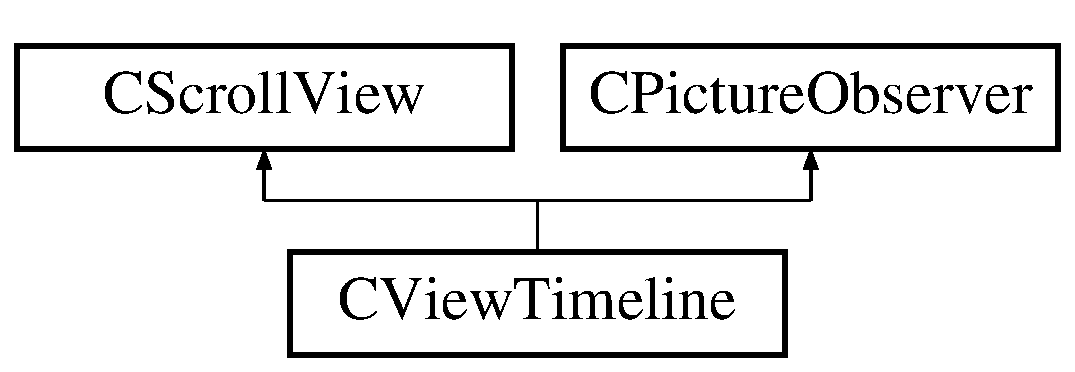
\includegraphics[height=2.000000cm]{class_c_view_timeline}
\end{center}
\end{figure}
\subsection*{Public Member Functions}
\begin{DoxyCompactItemize}
\item 
void \hyperlink{class_c_view_timeline_aba069993dd75712f340999345e791327}{Set\+Main\+Frame} (\hyperlink{class_c_main_frame}{C\+Main\+Frame} $\ast$main\+Frame)
\begin{DoxyCompactList}\small\item\em Set the main\+Frame pointer. \end{DoxyCompactList}\item 
virtual void \hyperlink{class_c_view_timeline_a21388abd4726fd3dbe02b6e2ea313369}{Update\+Observer} () override
\begin{DoxyCompactList}\small\item\em Updates the observer. \end{DoxyCompactList}\item 
afx\+\_\+msg B\+O\+O\+L \hyperlink{class_c_view_timeline_a8328ae76e5f95d36b3ab7e8bbd8ef72f}{On\+Erase\+Bkgnd} (C\+D\+C $\ast$p\+D\+C)
\begin{DoxyCompactList}\small\item\em Erase the background. \end{DoxyCompactList}\item 
\hypertarget{class_c_view_timeline_acb22f2662a21152e607d17dbc293351c}{afx\+\_\+msg void \hyperlink{class_c_view_timeline_acb22f2662a21152e607d17dbc293351c}{On\+Edit\+Setkeyframe} ()}\label{class_c_view_timeline_acb22f2662a21152e607d17dbc293351c}

\begin{DoxyCompactList}\small\item\em Handle the Edit$>$Set Keyframe menu option. \end{DoxyCompactList}\item 
\hypertarget{class_c_view_timeline_ab3eccb4a5bcd5ffa60442359b86e0597}{afx\+\_\+msg void \hyperlink{class_c_view_timeline_ab3eccb4a5bcd5ffa60442359b86e0597}{On\+Edit\+Deletekeyframe} ()}\label{class_c_view_timeline_ab3eccb4a5bcd5ffa60442359b86e0597}

\begin{DoxyCompactList}\small\item\em Handle the Edit$>$Delete Keyframe menu option. \end{DoxyCompactList}\end{DoxyCompactItemize}
\subsection*{Static Public Attributes}
\begin{DoxyCompactItemize}
\item 
\hypertarget{class_c_view_timeline_a6634479092090825e8c392902cf6c685}{static const int \hyperlink{class_c_view_timeline_a6634479092090825e8c392902cf6c685}{Height} = 90}\label{class_c_view_timeline_a6634479092090825e8c392902cf6c685}

\begin{DoxyCompactList}\small\item\em Height to make this window. \end{DoxyCompactList}\end{DoxyCompactItemize}
\subsection*{Protected Member Functions}
\begin{DoxyCompactItemize}
\item 
\hypertarget{class_c_view_timeline_aee8b6ebfaa9e299c65d6be0fc27b79f1}{\hyperlink{class_c_view_timeline_aee8b6ebfaa9e299c65d6be0fc27b79f1}{C\+View\+Timeline} ()}\label{class_c_view_timeline_aee8b6ebfaa9e299c65d6be0fc27b79f1}

\begin{DoxyCompactList}\small\item\em Constructor. \end{DoxyCompactList}\item 
\hypertarget{class_c_view_timeline_afec58a7cb0dfafd6c64c19e9e8a57842}{virtual \hyperlink{class_c_view_timeline_afec58a7cb0dfafd6c64c19e9e8a57842}{$\sim$\+C\+View\+Timeline} ()}\label{class_c_view_timeline_afec58a7cb0dfafd6c64c19e9e8a57842}

\begin{DoxyCompactList}\small\item\em Destructor. \end{DoxyCompactList}\item 
virtual void \hyperlink{class_c_view_timeline_a32f2ff1b162abc49f841e5dd6ddcb7df}{On\+Draw} (C\+D\+C $\ast$p\+D\+C)
\begin{DoxyCompactList}\small\item\em Draw this window. \end{DoxyCompactList}\item 
\hypertarget{class_c_view_timeline_a7996d31301f034cf9fa59e3d846c5fb5}{virtual void \hyperlink{class_c_view_timeline_a7996d31301f034cf9fa59e3d846c5fb5}{On\+Initial\+Update} ()}\label{class_c_view_timeline_a7996d31301f034cf9fa59e3d846c5fb5}

\begin{DoxyCompactList}\small\item\em Handle the initial update for this window. \end{DoxyCompactList}\end{DoxyCompactItemize}


\subsection{Detailed Description}
View window for the animation timeline. 

\subsection{Member Function Documentation}
\hypertarget{class_c_view_timeline_a32f2ff1b162abc49f841e5dd6ddcb7df}{\index{C\+View\+Timeline@{C\+View\+Timeline}!On\+Draw@{On\+Draw}}
\index{On\+Draw@{On\+Draw}!C\+View\+Timeline@{C\+View\+Timeline}}
\subsubsection[{On\+Draw}]{\setlength{\rightskip}{0pt plus 5cm}void C\+View\+Timeline\+::\+On\+Draw (
\begin{DoxyParamCaption}
\item[{C\+D\+C $\ast$}]{p\+D\+C}
\end{DoxyParamCaption}
)\hspace{0.3cm}{\ttfamily [protected]}, {\ttfamily [virtual]}}}\label{class_c_view_timeline_a32f2ff1b162abc49f841e5dd6ddcb7df}


Draw this window. 


\begin{DoxyParams}{Parameters}
{\em p\+D\+C} & Device context \\
\hline
\end{DoxyParams}
\hypertarget{class_c_view_timeline_a8328ae76e5f95d36b3ab7e8bbd8ef72f}{\index{C\+View\+Timeline@{C\+View\+Timeline}!On\+Erase\+Bkgnd@{On\+Erase\+Bkgnd}}
\index{On\+Erase\+Bkgnd@{On\+Erase\+Bkgnd}!C\+View\+Timeline@{C\+View\+Timeline}}
\subsubsection[{On\+Erase\+Bkgnd}]{\setlength{\rightskip}{0pt plus 5cm}B\+O\+O\+L C\+View\+Timeline\+::\+On\+Erase\+Bkgnd (
\begin{DoxyParamCaption}
\item[{C\+D\+C $\ast$}]{p\+D\+C}
\end{DoxyParamCaption}
)}}\label{class_c_view_timeline_a8328ae76e5f95d36b3ab7e8bbd8ef72f}


Erase the background. 

This is disabled to eliminate flicker 
\begin{DoxyParams}{Parameters}
{\em p\+D\+C} & Device context \\
\hline
\end{DoxyParams}
\begin{DoxyReturn}{Returns}
F\+A\+L\+S\+E 
\end{DoxyReturn}
\hypertarget{class_c_view_timeline_aba069993dd75712f340999345e791327}{\index{C\+View\+Timeline@{C\+View\+Timeline}!Set\+Main\+Frame@{Set\+Main\+Frame}}
\index{Set\+Main\+Frame@{Set\+Main\+Frame}!C\+View\+Timeline@{C\+View\+Timeline}}
\subsubsection[{Set\+Main\+Frame}]{\setlength{\rightskip}{0pt plus 5cm}void C\+View\+Timeline\+::\+Set\+Main\+Frame (
\begin{DoxyParamCaption}
\item[{{\bf C\+Main\+Frame} $\ast$}]{main\+Frame}
\end{DoxyParamCaption}
)\hspace{0.3cm}{\ttfamily [inline]}}}\label{class_c_view_timeline_aba069993dd75712f340999345e791327}


Set the main\+Frame pointer. 


\begin{DoxyParams}{Parameters}
{\em main\+Frame} & Pointer to the \hyperlink{class_c_main_frame}{C\+Main\+Frame} window \\
\hline
\end{DoxyParams}
\hypertarget{class_c_view_timeline_a21388abd4726fd3dbe02b6e2ea313369}{\index{C\+View\+Timeline@{C\+View\+Timeline}!Update\+Observer@{Update\+Observer}}
\index{Update\+Observer@{Update\+Observer}!C\+View\+Timeline@{C\+View\+Timeline}}
\subsubsection[{Update\+Observer}]{\setlength{\rightskip}{0pt plus 5cm}void C\+View\+Timeline\+::\+Update\+Observer (
\begin{DoxyParamCaption}
{}
\end{DoxyParamCaption}
)\hspace{0.3cm}{\ttfamily [override]}, {\ttfamily [virtual]}}}\label{class_c_view_timeline_a21388abd4726fd3dbe02b6e2ea313369}


Updates the observer. 

Force an update of this window when the picture changes. 

Implements \hyperlink{class_c_picture_observer_a0dce27216a8cb8a2490f0efc83a5994a}{C\+Picture\+Observer}.



The documentation for this class was generated from the following files\+:\begin{DoxyCompactItemize}
\item 
\hyperlink{_view_timeline_8h}{View\+Timeline.\+h}\item 
\hyperlink{_view_timeline_8cpp}{View\+Timeline.\+cpp}\end{DoxyCompactItemize}

\hypertarget{class_c_view_top}{\section{C\+View\+Top Class Reference}
\label{class_c_view_top}\index{C\+View\+Top@{C\+View\+Top}}
}


Top of the screen view.  




{\ttfamily \#include $<$View\+Top.\+h$>$}

Inheritance diagram for C\+View\+Top\+:\begin{figure}[H]
\begin{center}
\leavevmode
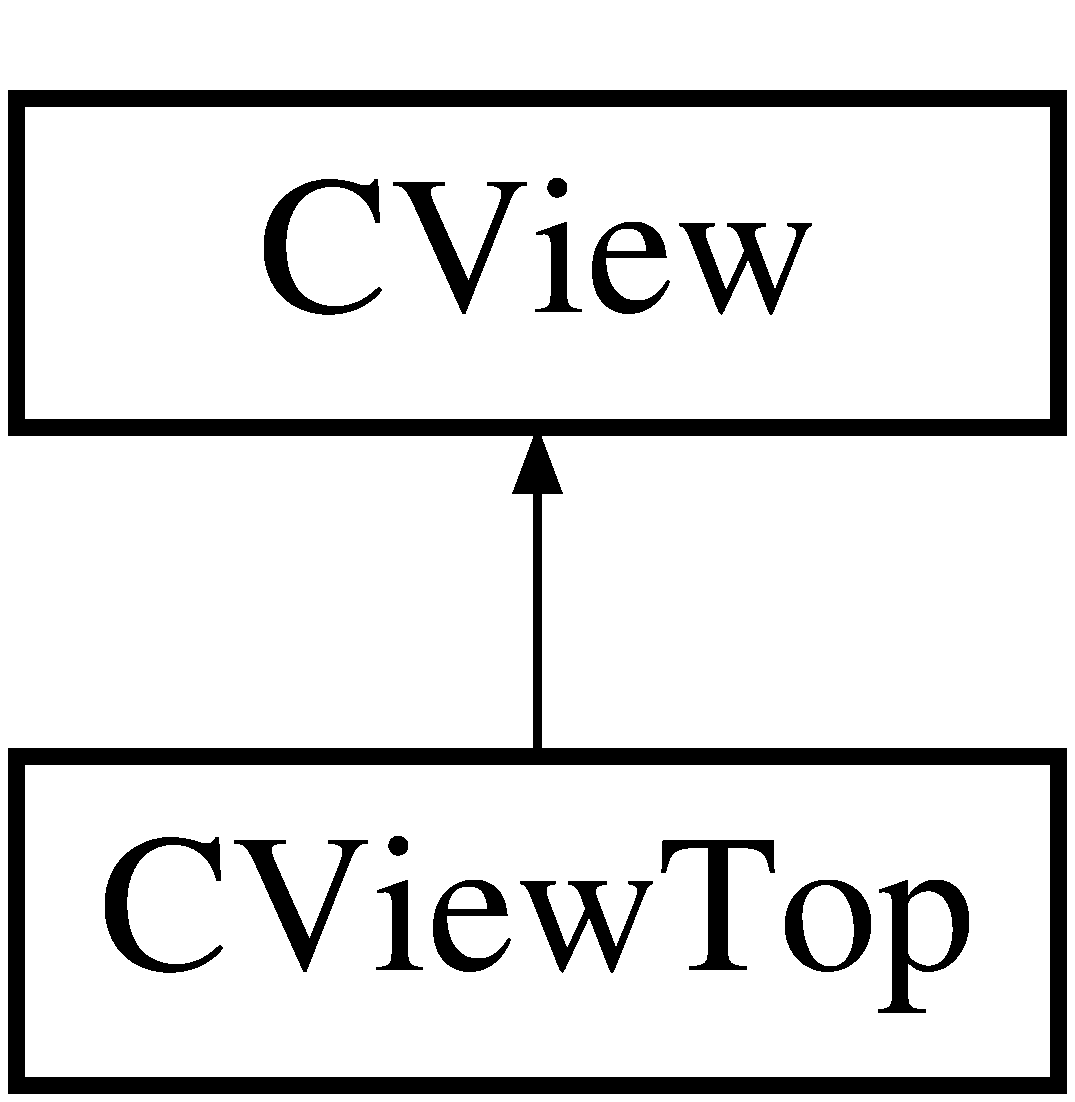
\includegraphics[height=2.000000cm]{class_c_view_top}
\end{center}
\end{figure}
\subsection*{Public Member Functions}
\begin{DoxyCompactItemize}
\item 
virtual void \hyperlink{class_c_view_top_ac4b8af93a75df56478f39feff289f6a6}{On\+Draw} (C\+D\+C $\ast$p\+D\+C)
\begin{DoxyCompactList}\small\item\em Drawing for this view. \end{DoxyCompactList}\item 
\hyperlink{class_c_view_edit}{C\+View\+Edit} $\ast$ \hyperlink{class_c_view_top_a775f50213ecac76ac57016bc402de42a}{Get\+View\+Edit} ()
\begin{DoxyCompactList}\small\item\em Get the View\+Edit window. \end{DoxyCompactList}\item 
\hyperlink{class_c_view_actors}{C\+View\+Actors} $\ast$ \hyperlink{class_c_view_top_a2057cf44f1f7a789b33e2ef8444b6db8}{Get\+View\+Actors} ()
\begin{DoxyCompactList}\small\item\em Get the View\+Actors window. \end{DoxyCompactList}\item 
afx\+\_\+msg int \hyperlink{class_c_view_top_a7e4cad13135855a66719ecb49a8ad3fc}{On\+Create} (L\+P\+C\+R\+E\+A\+T\+E\+S\+T\+R\+U\+C\+T lp\+Create\+Struct)
\begin{DoxyCompactList}\small\item\em Handle a C\+R\+E\+A\+T\+E message for this window. \end{DoxyCompactList}\item 
afx\+\_\+msg void \hyperlink{class_c_view_top_a171e02fdf1bef80245bbc37d77819f14}{On\+Size} (U\+I\+N\+T n\+Type, int cx, int cy)
\begin{DoxyCompactList}\small\item\em Handle a new size message. \end{DoxyCompactList}\end{DoxyCompactItemize}
\subsection*{Protected Member Functions}
\begin{DoxyCompactItemize}
\item 
\hypertarget{class_c_view_top_a4cee9890cf66890c3cd79efdedf92d1b}{\hyperlink{class_c_view_top_a4cee9890cf66890c3cd79efdedf92d1b}{C\+View\+Top} ()}\label{class_c_view_top_a4cee9890cf66890c3cd79efdedf92d1b}

\begin{DoxyCompactList}\small\item\em Constructor. \end{DoxyCompactList}\item 
\hypertarget{class_c_view_top_ad08e0ef0c01e33bb0278dc595467ad8c}{virtual \hyperlink{class_c_view_top_ad08e0ef0c01e33bb0278dc595467ad8c}{$\sim$\+C\+View\+Top} ()}\label{class_c_view_top_ad08e0ef0c01e33bb0278dc595467ad8c}

\begin{DoxyCompactList}\small\item\em Destructor. \end{DoxyCompactList}\end{DoxyCompactItemize}


\subsection{Detailed Description}
Top of the screen view. 

This class creates a view that contains a splitter so we can split the top window horizontally. 

\subsection{Member Function Documentation}
\hypertarget{class_c_view_top_a2057cf44f1f7a789b33e2ef8444b6db8}{\index{C\+View\+Top@{C\+View\+Top}!Get\+View\+Actors@{Get\+View\+Actors}}
\index{Get\+View\+Actors@{Get\+View\+Actors}!C\+View\+Top@{C\+View\+Top}}
\subsubsection[{Get\+View\+Actors}]{\setlength{\rightskip}{0pt plus 5cm}{\bf C\+View\+Actors}$\ast$ C\+View\+Top\+::\+Get\+View\+Actors (
\begin{DoxyParamCaption}
{}
\end{DoxyParamCaption}
)\hspace{0.3cm}{\ttfamily [inline]}}}\label{class_c_view_top_a2057cf44f1f7a789b33e2ef8444b6db8}


Get the View\+Actors window. 

\begin{DoxyReturn}{Returns}
Pointer to View\+Actors window 
\end{DoxyReturn}
\hypertarget{class_c_view_top_a775f50213ecac76ac57016bc402de42a}{\index{C\+View\+Top@{C\+View\+Top}!Get\+View\+Edit@{Get\+View\+Edit}}
\index{Get\+View\+Edit@{Get\+View\+Edit}!C\+View\+Top@{C\+View\+Top}}
\subsubsection[{Get\+View\+Edit}]{\setlength{\rightskip}{0pt plus 5cm}{\bf C\+View\+Edit}$\ast$ C\+View\+Top\+::\+Get\+View\+Edit (
\begin{DoxyParamCaption}
{}
\end{DoxyParamCaption}
)\hspace{0.3cm}{\ttfamily [inline]}}}\label{class_c_view_top_a775f50213ecac76ac57016bc402de42a}


Get the View\+Edit window. 

\begin{DoxyReturn}{Returns}
Pointer to View\+Edit window 
\end{DoxyReturn}
\hypertarget{class_c_view_top_a7e4cad13135855a66719ecb49a8ad3fc}{\index{C\+View\+Top@{C\+View\+Top}!On\+Create@{On\+Create}}
\index{On\+Create@{On\+Create}!C\+View\+Top@{C\+View\+Top}}
\subsubsection[{On\+Create}]{\setlength{\rightskip}{0pt plus 5cm}int C\+View\+Top\+::\+On\+Create (
\begin{DoxyParamCaption}
\item[{L\+P\+C\+R\+E\+A\+T\+E\+S\+T\+R\+U\+C\+T}]{lp\+Create\+Struct}
\end{DoxyParamCaption}
)}}\label{class_c_view_top_a7e4cad13135855a66719ecb49a8ad3fc}


Handle a C\+R\+E\+A\+T\+E message for this window. 


\begin{DoxyParams}{Parameters}
{\em lp\+Create\+Struct} & The creation parameter structure \\
\hline
\end{DoxyParams}
\begin{DoxyReturn}{Returns}
0 if successful 
\end{DoxyReturn}
\hypertarget{class_c_view_top_ac4b8af93a75df56478f39feff289f6a6}{\index{C\+View\+Top@{C\+View\+Top}!On\+Draw@{On\+Draw}}
\index{On\+Draw@{On\+Draw}!C\+View\+Top@{C\+View\+Top}}
\subsubsection[{On\+Draw}]{\setlength{\rightskip}{0pt plus 5cm}void C\+View\+Top\+::\+On\+Draw (
\begin{DoxyParamCaption}
\item[{C\+D\+C $\ast$}]{p\+D\+C}
\end{DoxyParamCaption}
)\hspace{0.3cm}{\ttfamily [virtual]}}}\label{class_c_view_top_ac4b8af93a75df56478f39feff289f6a6}


Drawing for this view. 


\begin{DoxyParams}{Parameters}
{\em p\+D\+C} & The device context \\
\hline
\end{DoxyParams}
\hypertarget{class_c_view_top_a171e02fdf1bef80245bbc37d77819f14}{\index{C\+View\+Top@{C\+View\+Top}!On\+Size@{On\+Size}}
\index{On\+Size@{On\+Size}!C\+View\+Top@{C\+View\+Top}}
\subsubsection[{On\+Size}]{\setlength{\rightskip}{0pt plus 5cm}void C\+View\+Top\+::\+On\+Size (
\begin{DoxyParamCaption}
\item[{U\+I\+N\+T}]{n\+Type, }
\item[{int}]{cx, }
\item[{int}]{cy}
\end{DoxyParamCaption}
)}}\label{class_c_view_top_a171e02fdf1bef80245bbc37d77819f14}


Handle a new size message. 


\begin{DoxyParams}{Parameters}
{\em n\+Type} & Type of size message \\
\hline
{\em cx} & New width \\
\hline
{\em cy} & New height \\
\hline
\end{DoxyParams}


The documentation for this class was generated from the following files\+:\begin{DoxyCompactItemize}
\item 
\hyperlink{_view_top_8h}{View\+Top.\+h}\item 
\hyperlink{_view_top_8cpp}{View\+Top.\+cpp}\end{DoxyCompactItemize}

\hypertarget{class_c_picture_1_1_iter}{\section{C\+Picture\+:\+:Iter Class Reference}
\label{class_c_picture_1_1_iter}\index{C\+Picture\+::\+Iter@{C\+Picture\+::\+Iter}}
}


Iterator for iteration over actors in our picture.  




{\ttfamily \#include $<$Picture.\+h$>$}

\subsection*{Public Member Functions}
\begin{DoxyCompactItemize}
\item 
\hyperlink{class_c_picture_1_1_iter_a05b2e6b7de1c7cadfb373700685ac727}{Iter} (vector$<$ shared\+\_\+ptr$<$ \hyperlink{class_c_actor}{C\+Actor} $>$ $>$ actors, int pos)
\begin{DoxyCompactList}\small\item\em Constructor for iterator. \end{DoxyCompactList}\item 
bool \hyperlink{class_c_picture_1_1_iter_ad6825ba137bf1f8e308a14ce8372fd96}{operator!=} (const \hyperlink{class_c_picture_1_1_iter}{Iter} \&other) const 
\begin{DoxyCompactList}\small\item\em Tests for the end of the iterator. \end{DoxyCompactList}\item 
std\+::shared\+\_\+ptr$<$ \hyperlink{class_c_actor}{C\+Actor} $>$ \hyperlink{class_c_picture_1_1_iter_ab6962e9b3aada98956eda038b77ab43c}{operator$\ast$} () const 
\begin{DoxyCompactList}\small\item\em Gets a value. \end{DoxyCompactList}\item 
const \hyperlink{class_c_picture_1_1_iter}{Iter} \& \hyperlink{class_c_picture_1_1_iter_aa0b7d41d80329022d80ec605b46924c2}{operator++} ()
\begin{DoxyCompactList}\small\item\em Increment the iterator. \end{DoxyCompactList}\end{DoxyCompactItemize}


\subsection{Detailed Description}
Iterator for iteration over actors in our picture. 

Iterator 

\subsection{Constructor \& Destructor Documentation}
\hypertarget{class_c_picture_1_1_iter_a05b2e6b7de1c7cadfb373700685ac727}{\index{C\+Picture\+::\+Iter@{C\+Picture\+::\+Iter}!Iter@{Iter}}
\index{Iter@{Iter}!C\+Picture\+::\+Iter@{C\+Picture\+::\+Iter}}
\subsubsection[{Iter}]{\setlength{\rightskip}{0pt plus 5cm}C\+Picture\+::\+Iter\+::\+Iter (
\begin{DoxyParamCaption}
\item[{vector$<$ shared\+\_\+ptr$<$ {\bf C\+Actor} $>$ $>$}]{actors, }
\item[{int}]{pos}
\end{DoxyParamCaption}
)\hspace{0.3cm}{\ttfamily [inline]}}}\label{class_c_picture_1_1_iter_a05b2e6b7de1c7cadfb373700685ac727}


Constructor for iterator. 


\begin{DoxyParams}{Parameters}
{\em actors} & -\/ The actors we are iterating over \\
\hline
{\em pos} & -\/ The position of our iterator \\
\hline
\end{DoxyParams}


\subsection{Member Function Documentation}
\hypertarget{class_c_picture_1_1_iter_ad6825ba137bf1f8e308a14ce8372fd96}{\index{C\+Picture\+::\+Iter@{C\+Picture\+::\+Iter}!operator"!=@{operator"!=}}
\index{operator"!=@{operator"!=}!C\+Picture\+::\+Iter@{C\+Picture\+::\+Iter}}
\subsubsection[{operator"!=}]{\setlength{\rightskip}{0pt plus 5cm}bool C\+Picture\+::\+Iter\+::operator!= (
\begin{DoxyParamCaption}
\item[{const {\bf Iter} \&}]{other}
\end{DoxyParamCaption}
) const\hspace{0.3cm}{\ttfamily [inline]}}}\label{class_c_picture_1_1_iter_ad6825ba137bf1f8e308a14ce8372fd96}


Tests for the end of the iterator. 

\begin{DoxyReturn}{Returns}
True if the current position is not equal to the other position 
\end{DoxyReturn}
\hypertarget{class_c_picture_1_1_iter_ab6962e9b3aada98956eda038b77ab43c}{\index{C\+Picture\+::\+Iter@{C\+Picture\+::\+Iter}!operator$\ast$@{operator$\ast$}}
\index{operator$\ast$@{operator$\ast$}!C\+Picture\+::\+Iter@{C\+Picture\+::\+Iter}}
\subsubsection[{operator$\ast$}]{\setlength{\rightskip}{0pt plus 5cm}std\+::shared\+\_\+ptr$<${\bf C\+Actor}$>$ C\+Picture\+::\+Iter\+::operator$\ast$ (
\begin{DoxyParamCaption}
{}
\end{DoxyParamCaption}
) const\hspace{0.3cm}{\ttfamily [inline]}}}\label{class_c_picture_1_1_iter_ab6962e9b3aada98956eda038b77ab43c}


Gets a value. 

\begin{DoxyReturn}{Returns}
Value at m\+Pos in the collection 
\end{DoxyReturn}
\hypertarget{class_c_picture_1_1_iter_aa0b7d41d80329022d80ec605b46924c2}{\index{C\+Picture\+::\+Iter@{C\+Picture\+::\+Iter}!operator++@{operator++}}
\index{operator++@{operator++}!C\+Picture\+::\+Iter@{C\+Picture\+::\+Iter}}
\subsubsection[{operator++}]{\setlength{\rightskip}{0pt plus 5cm}const {\bf Iter}\& C\+Picture\+::\+Iter\+::operator++ (
\begin{DoxyParamCaption}
{}
\end{DoxyParamCaption}
)\hspace{0.3cm}{\ttfamily [inline]}}}\label{class_c_picture_1_1_iter_aa0b7d41d80329022d80ec605b46924c2}


Increment the iterator. 

\begin{DoxyReturn}{Returns}
Reference to this iterator 
\end{DoxyReturn}


The documentation for this class was generated from the following file\+:\begin{DoxyCompactItemize}
\item 
\hyperlink{_picture_8h}{Picture.\+h}\end{DoxyCompactItemize}

\chapter{File Documentation}
\hypertarget{_actor_8cpp}{\section{Actor.\+cpp File Reference}
\label{_actor_8cpp}\index{Actor.\+cpp@{Actor.\+cpp}}
}
{\ttfamily \#include \char`\"{}stdafx.\+h\char`\"{}}\\*
{\ttfamily \#include \char`\"{}Actor.\+h\char`\"{}}\\*


\subsection{Detailed Description}
\begin{DoxyAuthor}{Author}
Charles Bean 
\end{DoxyAuthor}

\hypertarget{_actor_8h}{\section{Actor.\+h File Reference}
\label{_actor_8h}\index{Actor.\+h@{Actor.\+h}}
}


An actor is some graphical object that consists of one or more parts. Actors can be animated.  


{\ttfamily \#include $<$string$>$}\\*
{\ttfamily \#include $<$memory$>$}\\*
{\ttfamily \#include $<$vector$>$}\\*
{\ttfamily \#include \char`\"{}Drawable.\+h\char`\"{}}\\*
\subsection*{Classes}
\begin{DoxyCompactItemize}
\item 
class \hyperlink{class_c_actor}{C\+Actor}
\begin{DoxyCompactList}\small\item\em Class for actors in our drawings. \end{DoxyCompactList}\end{DoxyCompactItemize}


\subsection{Detailed Description}
An actor is some graphical object that consists of one or more parts. Actors can be animated. 

\begin{DoxyAuthor}{Author}
Charles Bean 
\end{DoxyAuthor}

\hypertarget{_actor_factory_8cpp}{\section{Actor\+Factory.\+cpp File Reference}
\label{_actor_factory_8cpp}\index{Actor\+Factory.\+cpp@{Actor\+Factory.\+cpp}}
}
{\ttfamily \#include \char`\"{}stdafx.\+h\char`\"{}}\\*
{\ttfamily \#include \char`\"{}Actor\+Factory.\+h\char`\"{}}\\*


\subsection{Detailed Description}
\begin{DoxyAuthor}{Author}
Charles Bean 
\end{DoxyAuthor}

\hypertarget{_actor_factory_8h}{\section{Actor\+Factory.\+h File Reference}
\label{_actor_factory_8h}\index{Actor\+Factory.\+h@{Actor\+Factory.\+h}}
}


Abstract base class for actor factories.  


\subsection*{Classes}
\begin{DoxyCompactItemize}
\item 
class \hyperlink{class_c_actor_factory}{C\+Actor\+Factory}
\begin{DoxyCompactList}\small\item\em Abstract base class for actor factories. \end{DoxyCompactList}\end{DoxyCompactItemize}


\subsection{Detailed Description}
Abstract base class for actor factories. 

\begin{DoxyAuthor}{Author}
Charles Bean 
\end{DoxyAuthor}

\hypertarget{_butch_factory_8cpp}{\section{Butch\+Factory.\+cpp File Reference}
\label{_butch_factory_8cpp}\index{Butch\+Factory.\+cpp@{Butch\+Factory.\+cpp}}
}
{\ttfamily \#include \char`\"{}stdafx.\+h\char`\"{}}\\*
{\ttfamily \#include \char`\"{}Butch\+Factory.\+h\char`\"{}}\\*
{\ttfamily \#include \char`\"{}Image\+Drawable.\+h\char`\"{}}\\*
{\ttfamily \#include \char`\"{}Poly\+Drawable.\+h\char`\"{}}\\*
{\ttfamily \#include \char`\"{}Head\+Top.\+h\char`\"{}}\\*


\subsection{Detailed Description}
\begin{DoxyAuthor}{Author}
Charles Bean 
\end{DoxyAuthor}

\hypertarget{_butch_factory_8h}{\section{Butch\+Factory.\+h File Reference}
\label{_butch_factory_8h}\index{Butch\+Factory.\+h@{Butch\+Factory.\+h}}
}


Class that creates a new actor -\/ Butch.  


{\ttfamily \#include \char`\"{}Actor\+Factory.\+h\char`\"{}}\\*
{\ttfamily \#include \char`\"{}Actor.\+h\char`\"{}}\\*
{\ttfamily \#include $<$memory$>$}\\*
\subsection*{Classes}
\begin{DoxyCompactItemize}
\item 
class \hyperlink{class_c_butch_factory}{C\+Butch\+Factory}
\begin{DoxyCompactList}\small\item\em Creates a new actor -\/ Butch. \end{DoxyCompactList}\end{DoxyCompactItemize}


\subsection{Detailed Description}
Class that creates a new actor -\/ Butch. 

\begin{DoxyAuthor}{Author}
Charles Bean 
\end{DoxyAuthor}

\hypertarget{_canadian_experience_8cpp}{\section{Canadian\+Experience.\+cpp File Reference}
\label{_canadian_experience_8cpp}\index{Canadian\+Experience.\+cpp@{Canadian\+Experience.\+cpp}}
}
{\ttfamily \#include \char`\"{}stdafx.\+h\char`\"{}}\\*
{\ttfamily \#include \char`\"{}afxwinappex.\+h\char`\"{}}\\*
{\ttfamily \#include \char`\"{}afxdialogex.\+h\char`\"{}}\\*
{\ttfamily \#include \char`\"{}Canadian\+Experience.\+h\char`\"{}}\\*
{\ttfamily \#include \char`\"{}Main\+Frm.\+h\char`\"{}}\\*
\subsection*{Classes}
\begin{DoxyCompactItemize}
\item 
class \hyperlink{class_c_about_dlg}{C\+About\+Dlg}
\begin{DoxyCompactList}\small\item\em The About dialog box. \end{DoxyCompactList}\end{DoxyCompactItemize}
\subsection*{Variables}
\begin{DoxyCompactItemize}
\item 
\hypertarget{_canadian_experience_8cpp_a67124bfb0809a8ff695444fd678f7a94}{\hyperlink{class_c_canadian_experience_app}{C\+Canadian\+Experience\+App} \hyperlink{_canadian_experience_8cpp_a67124bfb0809a8ff695444fd678f7a94}{the\+App}}\label{_canadian_experience_8cpp_a67124bfb0809a8ff695444fd678f7a94}

\begin{DoxyCompactList}\small\item\em The one and only \hyperlink{class_c_canadian_experience_app}{C\+Canadian\+Experience\+App} object. \end{DoxyCompactList}\end{DoxyCompactItemize}


\subsection{Detailed Description}
\begin{DoxyAuthor}{Author}
Charles Bean 
\end{DoxyAuthor}

\hypertarget{_canadian_experience_8h}{\section{Canadian\+Experience.\+h File Reference}
\label{_canadian_experience_8h}\index{Canadian\+Experience.\+h@{Canadian\+Experience.\+h}}
}


Program application class.  


{\ttfamily \#include \char`\"{}resource.\+h\char`\"{}}\\*
\subsection*{Classes}
\begin{DoxyCompactItemize}
\item 
class \hyperlink{class_c_canadian_experience_app}{C\+Canadian\+Experience\+App}
\begin{DoxyCompactList}\small\item\em Program application class. \end{DoxyCompactList}\end{DoxyCompactItemize}
\subsection*{Variables}
\begin{DoxyCompactItemize}
\item 
\hypertarget{_canadian_experience_8h_a67124bfb0809a8ff695444fd678f7a94}{\hyperlink{class_c_canadian_experience_app}{C\+Canadian\+Experience\+App} \hyperlink{_canadian_experience_8h_a67124bfb0809a8ff695444fd678f7a94}{the\+App}}\label{_canadian_experience_8h_a67124bfb0809a8ff695444fd678f7a94}

\begin{DoxyCompactList}\small\item\em The one and only \hyperlink{class_c_canadian_experience_app}{C\+Canadian\+Experience\+App} object. \end{DoxyCompactList}\end{DoxyCompactItemize}


\subsection{Detailed Description}
Program application class. 

\begin{DoxyAuthor}{Author}
Charles Bean 
\end{DoxyAuthor}

\hypertarget{_double_buffer_d_c_8h}{\section{Double\+Buffer\+D\+C.\+h File Reference}
\label{_double_buffer_d_c_8h}\index{Double\+Buffer\+D\+C.\+h@{Double\+Buffer\+D\+C.\+h}}
}


Customer device context that supports double buffering.  




\subsection{Detailed Description}
Customer device context that supports double buffering. 


\hypertarget{_drawable_8cpp}{\section{Drawable.\+cpp File Reference}
\label{_drawable_8cpp}\index{Drawable.\+cpp@{Drawable.\+cpp}}
}
{\ttfamily \#include \char`\"{}stdafx.\+h\char`\"{}}\\*
{\ttfamily \#include \char`\"{}Drawable.\+h\char`\"{}}\\*
{\ttfamily \#include $<$cmath$>$}\\*


\subsection{Detailed Description}
\begin{DoxyAuthor}{Author}
Charles Bean 
\end{DoxyAuthor}

\hypertarget{_drawable_8h}{\section{Drawable.\+h File Reference}
\label{_drawable_8h}\index{Drawable.\+h@{Drawable.\+h}}
}


A drawable is one part of an actor. Drawable parts can be moved independently.  


{\ttfamily \#include $<$memory$>$}\\*
{\ttfamily \#include $<$string$>$}\\*
{\ttfamily \#include $<$vector$>$}\\*
\subsection*{Classes}
\begin{DoxyCompactItemize}
\item 
class \hyperlink{class_c_drawable}{C\+Drawable}
\begin{DoxyCompactList}\small\item\em Abstract base class for drawable elements of our picture. \end{DoxyCompactList}\end{DoxyCompactItemize}


\subsection{Detailed Description}
A drawable is one part of an actor. Drawable parts can be moved independently. 

\begin{DoxyAuthor}{Author}
Charles Bean 
\end{DoxyAuthor}

\hypertarget{_harold_factory_8cpp}{\section{Harold\+Factory.\+cpp File Reference}
\label{_harold_factory_8cpp}\index{Harold\+Factory.\+cpp@{Harold\+Factory.\+cpp}}
}
{\ttfamily \#include \char`\"{}stdafx.\+h\char`\"{}}\\*
{\ttfamily \#include \char`\"{}Harold\+Factory.\+h\char`\"{}}\\*
{\ttfamily \#include $<$memory$>$}\\*
{\ttfamily \#include \char`\"{}Poly\+Drawable.\+h\char`\"{}}\\*
{\ttfamily \#include \char`\"{}Image\+Drawable.\+h\char`\"{}}\\*
{\ttfamily \#include \char`\"{}Head\+Top.\+h\char`\"{}}\\*


\subsection{Detailed Description}
\begin{DoxyAuthor}{Author}
Charles Bean 
\end{DoxyAuthor}

\hypertarget{_harold_factory_8h}{\section{Harold\+Factory.\+h File Reference}
\label{_harold_factory_8h}\index{Harold\+Factory.\+h@{Harold\+Factory.\+h}}
}


Factory class that builds the Harold character.  


{\ttfamily \#include $<$memory$>$}\\*
{\ttfamily \#include \char`\"{}Actor.\+h\char`\"{}}\\*
{\ttfamily \#include \char`\"{}Actor\+Factory.\+h\char`\"{}}\\*
\subsection*{Classes}
\begin{DoxyCompactItemize}
\item 
class \hyperlink{class_c_harold_factory}{C\+Harold\+Factory}
\begin{DoxyCompactList}\small\item\em Factory class that builds the Harold character. \end{DoxyCompactList}\end{DoxyCompactItemize}


\subsection{Detailed Description}
Factory class that builds the Harold character. 

\begin{DoxyAuthor}{Author}
Charles Bean 
\end{DoxyAuthor}

\hypertarget{_head_top_8cpp}{\section{Head\+Top.\+cpp File Reference}
\label{_head_top_8cpp}\index{Head\+Top.\+cpp@{Head\+Top.\+cpp}}
}
{\ttfamily \#include \char`\"{}stdafx.\+h\char`\"{}}\\*
{\ttfamily \#include \char`\"{}Head\+Top.\+h\char`\"{}}\\*
\subsection*{Variables}
\begin{DoxyCompactItemize}
\item 
\hypertarget{_head_top_8cpp_ade10fdf328965f595a01ff78f9f8dcc0}{const double \hyperlink{_head_top_8cpp_ade10fdf328965f595a01ff78f9f8dcc0}{Rto\+D} = 57.\+295779513}\label{_head_top_8cpp_ade10fdf328965f595a01ff78f9f8dcc0}

\begin{DoxyCompactList}\small\item\em Constant ratio to convert radians to degrees. \end{DoxyCompactList}\end{DoxyCompactItemize}


\subsection{Detailed Description}
\begin{DoxyAuthor}{Author}
Charles Bean 
\end{DoxyAuthor}

\hypertarget{_head_top_8h}{\section{Head\+Top.\+h File Reference}
\label{_head_top_8h}\index{Head\+Top.\+h@{Head\+Top.\+h}}
}


A class for representing the top of an actor's head.  


{\ttfamily \#include \char`\"{}Image\+Drawable.\+h\char`\"{}}\\*
{\ttfamily \#include $<$memory$>$}\\*
\subsection*{Classes}
\begin{DoxyCompactItemize}
\item 
class \hyperlink{class_c_head_top}{C\+Head\+Top}
\begin{DoxyCompactList}\small\item\em A class for representing the top of an actor's head. \end{DoxyCompactList}\end{DoxyCompactItemize}


\subsection{Detailed Description}
A class for representing the top of an actor's head. 

\begin{DoxyAuthor}{Author}
Charles Bean 
\end{DoxyAuthor}

\hypertarget{_image_drawable_8cpp}{\section{Image\+Drawable.\+cpp File Reference}
\label{_image_drawable_8cpp}\index{Image\+Drawable.\+cpp@{Image\+Drawable.\+cpp}}
}
{\ttfamily \#include \char`\"{}stdafx.\+h\char`\"{}}\\*
{\ttfamily \#include \char`\"{}Image\+Drawable.\+h\char`\"{}}\\*
\subsection*{Variables}
\begin{DoxyCompactItemize}
\item 
\hypertarget{_image_drawable_8cpp_ade10fdf328965f595a01ff78f9f8dcc0}{const double \hyperlink{_image_drawable_8cpp_ade10fdf328965f595a01ff78f9f8dcc0}{Rto\+D} = 57.\+295779513}\label{_image_drawable_8cpp_ade10fdf328965f595a01ff78f9f8dcc0}

\begin{DoxyCompactList}\small\item\em Constant ratio to convert radians to degrees. \end{DoxyCompactList}\end{DoxyCompactItemize}


\subsection{Detailed Description}
\begin{DoxyAuthor}{Author}
Charles Bean 
\end{DoxyAuthor}

\hypertarget{_image_drawable_8h}{\section{Image\+Drawable.\+h File Reference}
\label{_image_drawable_8h}\index{Image\+Drawable.\+h@{Image\+Drawable.\+h}}
}


Class representing an image drawable (not polygon)  


{\ttfamily \#include \char`\"{}Drawable.\+h\char`\"{}}\\*
{\ttfamily \#include $<$memory$>$}\\*
{\ttfamily \#include $<$string$>$}\\*
\subsection*{Classes}
\begin{DoxyCompactItemize}
\item 
class \hyperlink{class_c_image_drawable}{C\+Image\+Drawable}
\begin{DoxyCompactList}\small\item\em Class representing an image drawable (not polygon) \end{DoxyCompactList}\end{DoxyCompactItemize}


\subsection{Detailed Description}
Class representing an image drawable (not polygon) 

\begin{DoxyAuthor}{Author}
Charles Bean 
\end{DoxyAuthor}

\hypertarget{_main_frm_8cpp}{\section{Main\+Frm.\+cpp File Reference}
\label{_main_frm_8cpp}\index{Main\+Frm.\+cpp@{Main\+Frm.\+cpp}}
}
{\ttfamily \#include \char`\"{}stdafx.\+h\char`\"{}}\\*
{\ttfamily \#include \char`\"{}Canadian\+Experience.\+h\char`\"{}}\\*
{\ttfamily \#include \char`\"{}Main\+Frm.\+h\char`\"{}}\\*
{\ttfamily \#include \char`\"{}View\+Top.\+h\char`\"{}}\\*
{\ttfamily \#include $<$memory$>$}\\*
{\ttfamily \#include \char`\"{}Picture.\+h\char`\"{}}\\*
{\ttfamily \#include \char`\"{}Picture\+Factory.\+h\char`\"{}}\\*


\subsection{Detailed Description}
Implementation of the \hyperlink{class_c_main_frame}{C\+Main\+Frame} class \begin{DoxyAuthor}{Author}
Charles Bean 
\end{DoxyAuthor}

\hypertarget{_main_frm_8h}{\section{Main\+Frm.\+h File Reference}
\label{_main_frm_8h}\index{Main\+Frm.\+h@{Main\+Frm.\+h}}
}


Main frame file.  


{\ttfamily \#include \char`\"{}Elevator\+App.\+h\char`\"{}}\\*
{\ttfamily \#include \char`\"{}Elevator\+Wnd.\+h\char`\"{}}\\*
\subsection*{Classes}
\begin{DoxyCompactItemize}
\item 
class \hyperlink{class_c_main_frame}{C\+Main\+Frame}
\begin{DoxyCompactList}\small\item\em The main frame class. \end{DoxyCompactList}\end{DoxyCompactItemize}


\subsection{Detailed Description}
Main frame file. 

\begin{DoxyAuthor}{Author}
Charles Bean 
\end{DoxyAuthor}

\hypertarget{_picture_8cpp}{\section{Picture.\+cpp File Reference}
\label{_picture_8cpp}\index{Picture.\+cpp@{Picture.\+cpp}}
}
{\ttfamily \#include \char`\"{}stdafx.\+h\char`\"{}}\\*
{\ttfamily \#include \char`\"{}Picture.\+h\char`\"{}}\\*


\subsection{Detailed Description}
\begin{DoxyAuthor}{Author}
Charles Bean 
\end{DoxyAuthor}

\hypertarget{_picture_8h}{\section{Picture.\+h File Reference}
\label{_picture_8h}\index{Picture.\+h@{Picture.\+h}}
}


There will be one picture object that contains all of our actors, which then contains the drawables.  


{\ttfamily \#include $<$vector$>$}\\*
{\ttfamily \#include \char`\"{}Picture\+Observer.\+h\char`\"{}}\\*
{\ttfamily \#include \char`\"{}Actor.\+h\char`\"{}}\\*
\subsection*{Classes}
\begin{DoxyCompactItemize}
\item 
class \hyperlink{class_c_picture}{C\+Picture}
\begin{DoxyCompactList}\small\item\em The picture we are drawing. \end{DoxyCompactList}\item 
class \hyperlink{class_c_picture_1_1_iter}{C\+Picture\+::\+Iter}
\begin{DoxyCompactList}\small\item\em Iterator for iteration over actors in our picture. \end{DoxyCompactList}\end{DoxyCompactItemize}


\subsection{Detailed Description}
There will be one picture object that contains all of our actors, which then contains the drawables. 

\begin{DoxyAuthor}{Author}
Charles Bean 
\end{DoxyAuthor}

\hypertarget{_picture_factory_8cpp}{\section{Picture\+Factory.\+cpp File Reference}
\label{_picture_factory_8cpp}\index{Picture\+Factory.\+cpp@{Picture\+Factory.\+cpp}}
}
{\ttfamily \#include \char`\"{}stdafx.\+h\char`\"{}}\\*
{\ttfamily \#include \char`\"{}Picture\+Factory.\+h\char`\"{}}\\*
{\ttfamily \#include \char`\"{}Harold\+Factory.\+h\char`\"{}}\\*
{\ttfamily \#include \char`\"{}Image\+Drawable.\+h\char`\"{}}\\*
{\ttfamily \#include \char`\"{}Butch\+Factory.\+h\char`\"{}}\\*
{\ttfamily \#include $<$memory$>$}\\*


\subsection{Detailed Description}
\begin{DoxyAuthor}{Author}
Charles Bean 
\end{DoxyAuthor}

\hypertarget{_picture_factory_8h}{\section{Picture\+Factory.\+h File Reference}
\label{_picture_factory_8h}\index{Picture\+Factory.\+h@{Picture\+Factory.\+h}}
}


The class that holds code for a picture factory.  


{\ttfamily \#include $<$memory$>$}\\*
{\ttfamily \#include \char`\"{}Picture.\+h\char`\"{}}\\*
\subsection*{Classes}
\begin{DoxyCompactItemize}
\item 
class \hyperlink{class_c_picture_factory}{C\+Picture\+Factory}
\begin{DoxyCompactList}\small\item\em A factory class that builds our picture. \end{DoxyCompactList}\end{DoxyCompactItemize}


\subsection{Detailed Description}
The class that holds code for a picture factory. 

\begin{DoxyAuthor}{Author}
Charles Bean 
\end{DoxyAuthor}

\hypertarget{_picture_observer_8cpp}{\section{Picture\+Observer.\+cpp File Reference}
\label{_picture_observer_8cpp}\index{Picture\+Observer.\+cpp@{Picture\+Observer.\+cpp}}
}
{\ttfamily \#include \char`\"{}stdafx.\+h\char`\"{}}\\*
{\ttfamily \#include \char`\"{}Picture\+Observer.\+h\char`\"{}}\\*
{\ttfamily \#include \char`\"{}Picture.\+h\char`\"{}}\\*


\subsection{Detailed Description}
\begin{DoxyAuthor}{Author}
Charles Bean 
\end{DoxyAuthor}

\hypertarget{_picture_observer_8h}{\section{Picture\+Observer.\+h File Reference}
\label{_picture_observer_8h}\index{Picture\+Observer.\+h@{Picture\+Observer.\+h}}
}


This class implements the base class functionality for an observer in the observer pattern.  


{\ttfamily \#include $<$memory$>$}\\*
\subsection*{Classes}
\begin{DoxyCompactItemize}
\item 
class \hyperlink{class_c_picture_observer}{C\+Picture\+Observer}
\begin{DoxyCompactList}\small\item\em Observer base class for a picture. \end{DoxyCompactList}\end{DoxyCompactItemize}


\subsection{Detailed Description}
This class implements the base class functionality for an observer in the observer pattern. 

\begin{DoxyAuthor}{Author}
Charles Bean 
\end{DoxyAuthor}

\hypertarget{_poly_drawable_8cpp}{\section{Poly\+Drawable.\+cpp File Reference}
\label{_poly_drawable_8cpp}\index{Poly\+Drawable.\+cpp@{Poly\+Drawable.\+cpp}}
}
{\ttfamily \#include \char`\"{}stdafx.\+h\char`\"{}}\\*
{\ttfamily \#include \char`\"{}Poly\+Drawable.\+h\char`\"{}}\\*


\subsection{Detailed Description}
\begin{DoxyAuthor}{Author}
Charles Bean 
\end{DoxyAuthor}

\hypertarget{_poly_drawable_8h}{\section{Poly\+Drawable.\+h File Reference}
\label{_poly_drawable_8h}\index{Poly\+Drawable.\+h@{Poly\+Drawable.\+h}}
}


This class has a list of points and draws a polygon drawable based on those points.  


{\ttfamily \#include $<$memory$>$}\\*
{\ttfamily \#include $<$string$>$}\\*
{\ttfamily \#include $<$vector$>$}\\*
{\ttfamily \#include \char`\"{}Drawable.\+h\char`\"{}}\\*
\subsection*{Classes}
\begin{DoxyCompactItemize}
\item 
class \hyperlink{class_c_poly_drawable}{C\+Poly\+Drawable}
\begin{DoxyCompactList}\small\item\em A drawable based on polygon images. \end{DoxyCompactList}\end{DoxyCompactItemize}


\subsection{Detailed Description}
This class has a list of points and draws a polygon drawable based on those points. 

\begin{DoxyAuthor}{Author}
Charles Bean 
\end{DoxyAuthor}

\hypertarget{_view_actors_8cpp}{\section{View\+Actors.\+cpp File Reference}
\label{_view_actors_8cpp}\index{View\+Actors.\+cpp@{View\+Actors.\+cpp}}
}
{\ttfamily \#include \char`\"{}stdafx.\+h\char`\"{}}\\*
{\ttfamily \#include \char`\"{}Canadian\+Experience.\+h\char`\"{}}\\*
{\ttfamily \#include \char`\"{}View\+Actors.\+h\char`\"{}}\\*
{\ttfamily \#include \char`\"{}Double\+Buffer\+D\+C.\+h\char`\"{}}\\*


\subsection{Detailed Description}
\begin{DoxyAuthor}{Author}
Charles Bean 
\end{DoxyAuthor}

\hypertarget{_view_actors_8h}{\section{View\+Actors.\+h File Reference}
\label{_view_actors_8h}\index{View\+Actors.\+h@{View\+Actors.\+h}}
}


Class that provides a view windows for actors.  


{\ttfamily \#include \char`\"{}Picture\+Observer.\+h\char`\"{}}\\*
\subsection*{Classes}
\begin{DoxyCompactItemize}
\item 
class \hyperlink{class_c_view_actors}{C\+View\+Actors}
\begin{DoxyCompactList}\small\item\em Class that provides a view windows for actors. \end{DoxyCompactList}\end{DoxyCompactItemize}


\subsection{Detailed Description}
Class that provides a view windows for actors. 

\begin{DoxyAuthor}{Author}
Charles Bean 
\end{DoxyAuthor}

\hypertarget{_view_edit_8cpp}{\section{View\+Edit.\+cpp File Reference}
\label{_view_edit_8cpp}\index{View\+Edit.\+cpp@{View\+Edit.\+cpp}}
}
{\ttfamily \#include \char`\"{}stdafx.\+h\char`\"{}}\\*
{\ttfamily \#include \char`\"{}Canadian\+Experience.\+h\char`\"{}}\\*
{\ttfamily \#include \char`\"{}View\+Edit.\+h\char`\"{}}\\*
{\ttfamily \#include \char`\"{}Double\+Buffer\+D\+C.\+h\char`\"{}}\\*
{\ttfamily \#include \char`\"{}Main\+Frm.\+h\char`\"{}}\\*
{\ttfamily \#include \char`\"{}Picture.\+h\char`\"{}}\\*
\subsection*{Variables}
\begin{DoxyCompactItemize}
\item 
\hypertarget{_view_edit_8cpp_a5aad50df163545659b29dc0f88c8a2d4}{const double \hyperlink{_view_edit_8cpp_a5aad50df163545659b29dc0f88c8a2d4}{Rotation\+Scaling} = 0.\+02}\label{_view_edit_8cpp_a5aad50df163545659b29dc0f88c8a2d4}

\begin{DoxyCompactList}\small\item\em A scaling factor, converts mouse motion to rotation in radians. \end{DoxyCompactList}\end{DoxyCompactItemize}


\subsection{Detailed Description}
\begin{DoxyAuthor}{Author}
Charles Bean 
\end{DoxyAuthor}

\hypertarget{_view_edit_8h}{\section{View\+Edit.\+h File Reference}
\label{_view_edit_8h}\index{View\+Edit.\+h@{View\+Edit.\+h}}
}


View class the provides a window for editing our pixture.  


{\ttfamily \#include \char`\"{}Picture\+Observer.\+h\char`\"{}}\\*
{\ttfamily \#include \char`\"{}Actor.\+h\char`\"{}}\\*
{\ttfamily \#include \char`\"{}Drawable.\+h\char`\"{}}\\*
{\ttfamily \#include $<$memory$>$}\\*
\subsection*{Classes}
\begin{DoxyCompactItemize}
\item 
class \hyperlink{class_c_view_edit}{C\+View\+Edit}
\begin{DoxyCompactList}\small\item\em View class the provides a window for editing our pixture. \end{DoxyCompactList}\end{DoxyCompactItemize}


\subsection{Detailed Description}
View class the provides a window for editing our pixture. 

\begin{DoxyAuthor}{Author}
Charles Bean 
\end{DoxyAuthor}

\hypertarget{_view_timeline_8cpp}{\section{View\+Timeline.\+cpp File Reference}
\label{_view_timeline_8cpp}\index{View\+Timeline.\+cpp@{View\+Timeline.\+cpp}}
}
{\ttfamily \#include \char`\"{}stdafx.\+h\char`\"{}}\\*
{\ttfamily \#include \char`\"{}Canadian\+Experience.\+h\char`\"{}}\\*
{\ttfamily \#include \char`\"{}View\+Timeline.\+h\char`\"{}}\\*
{\ttfamily \#include \char`\"{}Double\+Buffer\+D\+C.\+h\char`\"{}}\\*
{\ttfamily \#include \char`\"{}Main\+Frm.\+h\char`\"{}}\\*


\subsection{Detailed Description}
\begin{DoxyAuthor}{Author}
Charles Bean 
\end{DoxyAuthor}

\hypertarget{_view_timeline_8h}{\section{View\+Timeline.\+h File Reference}
\label{_view_timeline_8h}\index{View\+Timeline.\+h@{View\+Timeline.\+h}}
}


View window for the animation timeline.  


{\ttfamily \#include \char`\"{}Picture\+Observer.\+h\char`\"{}}\\*
\subsection*{Classes}
\begin{DoxyCompactItemize}
\item 
class \hyperlink{class_c_view_timeline}{C\+View\+Timeline}
\begin{DoxyCompactList}\small\item\em View window for the animation timeline. \end{DoxyCompactList}\end{DoxyCompactItemize}


\subsection{Detailed Description}
View window for the animation timeline. 

\begin{DoxyAuthor}{Author}
Charles Bean 
\end{DoxyAuthor}

\hypertarget{_view_top_8cpp}{\section{View\+Top.\+cpp File Reference}
\label{_view_top_8cpp}\index{View\+Top.\+cpp@{View\+Top.\+cpp}}
}
{\ttfamily \#include \char`\"{}stdafx.\+h\char`\"{}}\\*
{\ttfamily \#include \char`\"{}Canadian\+Experience.\+h\char`\"{}}\\*
{\ttfamily \#include \char`\"{}View\+Top.\+h\char`\"{}}\\*
{\ttfamily \#include \char`\"{}View\+Actors.\+h\char`\"{}}\\*
{\ttfamily \#include \char`\"{}View\+Edit.\+h\char`\"{}}\\*
{\ttfamily \#include \char`\"{}View\+Timeline.\+h\char`\"{}}\\*


\subsection{Detailed Description}
\begin{DoxyAuthor}{Author}
Charles B. Owen 
\end{DoxyAuthor}

\hypertarget{_view_top_8h}{\section{View\+Top.\+h File Reference}
\label{_view_top_8h}\index{View\+Top.\+h@{View\+Top.\+h}}
}


Class for the top of the screen view.  


{\ttfamily \#include \char`\"{}View\+Edit.\+h\char`\"{}}\\*
{\ttfamily \#include \char`\"{}View\+Actors.\+h\char`\"{}}\\*
\subsection*{Classes}
\begin{DoxyCompactItemize}
\item 
class \hyperlink{class_c_view_top}{C\+View\+Top}
\begin{DoxyCompactList}\small\item\em Top of the screen view. \end{DoxyCompactList}\end{DoxyCompactItemize}


\subsection{Detailed Description}
Class for the top of the screen view. 

\begin{DoxyAuthor}{Author}
Charles B. Owen
\end{DoxyAuthor}
You should not have to change this file. 
%--- End generated contents ---

% Index
\newpage
\phantomsection
\addcontentsline{toc}{chapter}{Index}
\printindex

\end{document}
